\documentclass[12pt,a4paper]{book}

	
\usepackage[letterpaper,
			left=2cm,
			right=2cm,
			bottom=2cm,
			headheight=18pt
			]{geometry}
\usepackage[T1]{fontenc}
\usepackage[utf8]{inputenc}


\usepackage{tabularx}
\usepackage{appendix}
\usepackage{ltablex}
\usepackage{array}
\usepackage{multirow}
\usepackage{longtable}
\usepackage[table]{xcolor}
\renewcommand{\arraystretch}{1.5}
\newcolumntype{a}{>{\columncolor[HTML]{EDEBAA}} m{0.4\textwidth} }
\newcolumntype{b}{>{\columncolor[HTML]{EDEBAA}} m{0.15\textwidth} }


\usepackage{csquotes}
\usepackage[style=numeric,backend=biber]{biblatex}
\addbibresource{References.bib}


\usepackage{graphicx}
\usepackage{emptypage}
\usepackage{fancyhdr}
\usepackage{amsmath}
\usepackage{calc}
\usepackage{fourier-orns}

\renewcommand{\headrule}{%
	\vspace{-8pt}\hrulefill
	\raisebox{-2.1pt}{\quad\decofourleft\textbf{\tiny LIBEIL}\decofourright\quad}\hrulefill
	}
%\renewcommand{\headheight}{17pt}
\renewcommand{\listfigurename}{Figures}
\renewcommand{\listtablename}{Tables}
\newcommand{\projectName}{LibEIl}
\newcommand{\websiteURL}{\url{https://libeil.fds.edu.ht}}
\newcommand{\dashboardURL}{\url{https://libeil.fds.edu.ht/admin/login}}

\usepackage[explicit]{titlesec}
\usepackage[most]{tcolorbox}
\usepackage{tikz}
\usepackage{xpatch}
\usepackage{lmodern}

\newlength\ChapWd
\settowidth\ChapWd{\huge\chaptertitlename}


	\titleformat{\part}[block]
	{\normalfont\huge\bfseries}
	{}
	{0pt}
	{\newgeometry{margin=50pt}
		\begin{minipage}{0.35\textwidth}
			\begin{tcolorbox}[colback=lightgray, colframe=lightgray, width=\textwidth, height=\textheight, valign=top, halign=center, sharp corners]
				\color{lightgray} some text
			\end{tcolorbox}
		\end{minipage}%
		\hspace{20pt}
		\begin{minipage}{0.6\textwidth}
			\vspace*{\fill}
			\centering \Large\color{myblue}\partname~\thepart:
			{\color{myblue}\rule{\textwidth}{5pt}}
			\Huge ~#1
			\vspace*{\fill}
		\end{minipage}
		\restoregeometry
	}


	\titleformat{\chapter}[display]
	{\normalfont\filcenter\huge\bfseries}
	{\tikz[remember picture,overlay]
		{
			\node[fill=myblue,font=\fontsize{60}{72}\selectfont\color{white},anchor=north east,minimum size=\ChapWd]
			at ([xshift=-15pt,yshift=-15pt]current page.north east)
			(numb) {\thechapter};
			\node[rotate=90,anchor=south,inner sep=0pt,font=\Large] at (numb.west) {\chaptertitlename};
		}
	}
	{30pt}
	{\fontsize{33}{40}\selectfont\color{myblue}#1}
	[\vskip3pt\huge {\color{myblue}\rule{\textwidth}{2pt}}]
	\titlespacing*{\chapter}
	{0pt}{50pt}{10pt}

	\titleformat{\section}
	{\normalfont\Large\bfseries\color{myblue}}
	{\thesection }
	{10pt}
	{#1}

	\titleformat{\subsection}
	{\normalfont\large\bfseries\color{myblue}}
	{\thesubsection }
	{10pt}
	{#1}

	\titleformat{\subsubsection}
	{\normalfont\bfseries\color{myblue}}
	{\thesubsubsection }
	{10pt}
	{#1}



\usepackage[french]{babel}
\usepackage{listings}


\definecolor{myblue}{RGB}{0,0,70}
\definecolor{mybrown}{RGB}{255,240,230}
\definecolor{TetTablo}{RGB}{240,240,255}
\definecolor{frameblue}{RGB}{150,150,150}
\definecolor{fillblue}{RGB}{210,230,255}

\usepackage{hyperref}
\hypersetup{
	colorlinks= true,
	linktoc= all,
	linkcolor= black,
	urlcolor= myblue,
	citecolor= black,
}



%____________QUESTIONS POUR NOS TUTEURS________________________
% Quel pourrait \^etre une source fiable pour pr\'esenter l'URG\'eo outre son site officiel?
%------------------------------------------------------------------------------------------------------------------------------



\begin{document}

	\thispagestyle{empty}
\begin{titlepage}
%	\pagecolor{green}
    \begin{center}
        \vspace*{1cm}

        \Huge
        {\bfseries\scshape \projectName}

        \vspace{0.5cm}
        \LARGE
        Librairie pour une \'Education par l'Illustration

        \vspace{1.5cm}

        \large
        \textbf{BIEN-AIM\'E Alias Vicky\\ DOR S. Marvens\\ GEDEUS Berny}

        \vfill
        \begin{tabular}{c}
        \hline
         Projet de sortie pr\'esent\'e pour le dipl\^ome en\\
        Ing\'enierie \'electronique\\
        \hline
        \end{tabular}


        \vfill

        
\includegraphics[height=2cm]{Pictures/LogoFDS.jpeg}

        \vspace{0.4cm}
        Facult\'e Des Sciences / Universit\'e d'\'Etat d'Ha\"iti (FDS/UEH)\\
        \vspace{0.8cm}

        \normalsize
        \emph{\bfseries \today}
        \vspace{0.5cm}

    \end{center}
\end{titlepage}
%\nopagecolor 

\pagenumbering{Roman}

	%Avertissment______________________________________________
	\rule{\textwidth}{5pt}
	\thispagestyle{empty}
	\vspace{1pt}
	\begin{minipage}{0.6\textwidth}
		
		\vspace{15cm}
		\textcolor{white}{text}
	\end{minipage}
	\begin{minipage}{0.4\textwidth}
		{\small 
		All web addresses provided in this document were correct at the time of consultation mentioned in the bibliography. The authors regret any inconvenience caused if addresses have changed or if sites have ceased to exist but cannot accept any responsability for such changes.
		
		\vspace{1cm}
		
		Toutes les adresses web fournies dans ce document \'etaient correctes \`a la date de consultation mentionn\'ee dans la bibliographie. Les auteurs regrettent tout inconv\'enient caus\'e par un \'eventuel changement d'adresse ou la disparition des sites, mais ne peuvent assumer aucune responsabilit\'e pour de tels changements.
		}
		\vspace*{\fill}
	\end{minipage}

	\vspace{3cm}




	\newpage

\begin{center}
	\textcolor{white}{kjbkjjkbjjhjh}\\
\vspace{2cm}
\textbf{\textit{\Huge{\textcolor{myblue}{R\'esum\'e}}}}
\vspace{2cm}
    
    \begin{minipage}{0.75\textwidth}
		\addcontentsline{toc}{chapter}{R\'esum\'e}
    	
	    \paragraph{}Ce document pr\'esente le projet r\'ealis\'e dans le but de distribuer un stock d'illustration produit par l'URG\'eo pour contribuer \`a l'\'education sur les facteurs de risques en Ha\"iti. Le projet en question, d\'enomm\'e \texttt{\projectName}, consiste \`a concevoir une solution informatique qui permettra de distribuer ces illustrations d'abord en Ha\"iti, mais \'egalement \`a travers le monde. \vspace{0.5cm}

	    
	    \paragraph{} La premi\`ere \'etape de la r\'ealisation de ce projet est d'\'evaluer les besoins du client, et de faire un \'etat des connaissances sur les concepts li\'es au projet. Une fois ce travail r\'ealis\'e, l'\'equipe de d\'eveloppement a propos\'e de construire une e-libraire pour adresser le probl\`eme.\par
	    \paragraph{}Ensuite viennent les analyses n\'ecessaires pour assurer le bon d\'eroulement de la construction du site web. D'une part, nous d\'ecouvrons les m\'ethodologie et frameworks de m\'ethodologie en r\'ealisation de projet, examinons les m\'ethodologies et frameworks de m\'ethodologie existant pour la cr\'eation d'un site web et choisissons la m\'ethodologie et le framework \`a utiliser pour la suite du projet. D'autre part nous analysons les risques qui pourraient nuire au d\'eroulement du projet et planifions les actions \`a entreprendre pour limiter ces risques ainsi que les r\'eactions \`a avoir en cas de survenue de l'un ou l'autre des risque pr\'evus, afin de mitiger leur impact sur le projet.\par
	    \paragraph{}La phase suivante est celle de la conception. Dans cette partie, nous mod\'elisons le projet pour identifier les fonctionnalit\'es \`a impl\'ementer, choisissons l'architecture \`a adopter pour le site, s\'electionnons les outils et technologies informatiques \`a utiliser et cr\'eons le mod\`ele de donn\'ees pour la construction de la base de donn\'ees.\par
	    \paragraph{}Enfin, nous pr\'esentons le projet apr\`es sa construction en d\'etaillant Les fonctionnalit\'es impl\'ement\'ees ainsi que les \'etapes \`a suivre pour l'utiliser, tant pour les simples utilisateurs du site que pour les administrateurs. \vspace{0.5cm}
	    
	    \paragraph{} \noindent Ce travail, financ\'e par le PNUD, est r\'ealis\'e dans le cadre de notre projet de fin d'\'etude en ing\'enierie \'electronique et, nous l'esp\'erons, contribuera \`a mieux \'eduquer la population ha\"itienne sur les concepts que traitent les diff\'erentes illustrations qui seront distribu\'ees.
   	\end{minipage}
    
    













\end{center}


	\newpage

\begin{center}
	\textcolor{white}{kjbkjjkbjjhjh}\\
	\vspace{2cm}
	\textbf{\textit{\Huge{\textcolor{myblue}{Abstract}}}}
	\vspace{2cm}
	
	\begin{minipage}{0.75\textwidth}
		\addcontentsline{toc}{chapter}{Abstract}
		
		\paragraph{}This document presents the project aimed at distributing a stock of illustrations produced by URG\'eo to contribute to education on risk factors in Haiti. The project, named \texttt{\projectName}, involves designing an IT solution that will allow these illustrations to be distributed first in Haiti and then globally. \vspace{0.5cm}
		 
		\paragraph{} The first step in carrying out our project is to assess the client's needs, and to take stock of the concepts that concern the project. Once this work completed, the development team proposed building an e-library to address the problem.\par
		\paragraph{}Next come the necessary analyses to ensure the smooth progress of the website construction. On the one hand, we explore project methodologies and frameworks, review existing methodologies and frameworks for website creation, and choose the methodology and framework to use for the remainder of the project. On the other hand, we analyze the risks that could affect the project's progress and plan the actions to be taken to mitigate these risks as well as the responses to have if any of the anticipated risks occur, in order to minimize their impact on the project.\par
		\paragraph{}The next phase is design. In this part, we model the project to identify the functionalities to be implemented, choose the architecture to adopt for the site, select the tools and technologies to use, and create the data model for building the database.\par
		\paragraph{}Finally, we present the project after its construction by detailing the implemented functionalities and the steps to follow for its use, both for regular site users and for administrators.\vspace{0.5cm}
		
		\paragraph{} \noindent This work, funded by the UNDP, is carried out as part of our final project in electronic engineering and, we hope, will help better educate the Haitian population on the concepts covered by the various illustrations that will be distributed.
	\end{minipage}
	
	
	
	
	
	
	
	
	
	
	
	
	
	
	
\end{center}


	\newpage

\begin{center}
	\textbf{\textit{\Huge{\textcolor{myblue}{Remerciements}}}}
	\addcontentsline{toc}{chapter}{Remerciements}
	\vspace{2cm}
	
	\begin{minipage}{0.75\textwidth}
		\`A \textbf{Yawhe}, par la gr\^ace de qui nous sommes, tout ce qui existe est et tout ouvrage est accompli. \\
		\textbf{\textit{Merci !}}
			
		\`A \textbf{M. Dominique Boisson},\\
		Pour votre confiance en nous, votre patience et vos conseils, \\
		\textbf{\textit{Merci !}}
				
		\`A nos encadreurs, \textbf{M. Kelly Guerrier} et M. \textbf{\'Elis\'ee Villiard},\\
		Pour votre disponibilit\'e, votre temps, votre patience, vos critiques, vos conseils, vos suggestions et votre support. Pour votre \'enorme contribution \`a la r\'ealisation de ce projet,\\
		\textbf{\textit{Merci !}}
				
		\`A \textbf{M. Wisly DieuJuste}, \\
		Pour votre aide \`a la mod\'elisation du projet et \`a l'\'etude de l'\'etat des connaissances,\\
		\textbf{\textit{Merci !}}
				
		\`A M. \textbf{Edgar Etienne} et M. \textbf{Antoine St-Victor},\\
		Pour votre soutien pendant nos ann\'ees d'\'etude.\\
		\textbf{\textit{Merci !}}\\

		\vspace{5pt}
		\`A nos proches, familles et amis qui nous ont aid\'es et soutenu dans nos ann\'ees d'\'etude. \\
		Pour votre amour et votre accompagnement. Sans vous, notre r\^eve serait tr\`es difficile \`a atteindre.\\
		mention sp\'ecial pour \textbf{Urie GEDEUS, L\'eonie DOR, Laury BIEN-AIME, Anne Marie FOY GEDEUS, David Jolicoeur Sr., Marl\`ene CHAMPAGNE, Jeff DOR, Youri GEDEUS, Val\'erie BIEN-AIME, Mistral GEDEUS} \\
		\textbf{\textit{Merci !}}
				
		\vspace{5pt}
		\`A vous tous, nombreux que vous \^etes, qui nous aurez aid\'es d'une fa\c{c}on ou d'une autre, en grand ou en peu, directement ou indirectement, pendant notre \'etude ou durant la r\'ealisation du projet, \\
		re-mention sp\'ecial pour M. \textbf{Edgar Etienne}, M. \textbf{Guy Raymond Jean}, \\
		\textbf{\textit{Merci !}}	
		
		\vspace{30pt}
		Nous vous en sommes reconnaissants.	
				
	\end{minipage}
	
	
	
	
	
	
	
	
	
	
	
	
	
	
	
\end{center}
    






	\tableofcontents

	\listoffigures

	\listoftables





	\pagestyle{fancy}
	\fancyhf{}
	\fancyhead[LE]{\nouppercase{
\includegraphics[height=2ex]{Pictures/libeil}\hfill\rightmark        }}
	\fancyhead[RO]{\nouppercase{\leftmark\hfill
\includegraphics[height=2ex]{Pictures/libeil}}}
	\fancyfoot[LE]{\hfill\thepage}
	\fancyfoot[RO]{\thepage\hfill}
	\pagenumbering{arabic}

	\part*{Introduction}

		\newrefsection
			\chapter*{Mise en contexte}
    \addcontentsline{toc}{chapter}{Mise en contexte}
%--------------------------------------------------Introduction generale-------------------------------------------------------------------------

	\addcontentsline{toc}{section}{Introduction g\'en\'erale}

	\paragraph{} La R\'epublique d'Ha\"iti est un pays insulaire situ\'e dans les Cara\"ibes, partageant l'\^ile d'Ha\"iti avec la R\'epublique Dominicaine \`a l'est . Le pays a une superficie de 27 750 kilom\`etres carr\'es\cite{htsuperficie}, c'est le troisi\`eme pays le plus peupl\'e des Cara\"ibes, avec une population estim\'ee \`a pr\`es de 11,448 millions d'habitants.\cite{htpopulationA}\cite{htpopulationB} \\
	Ha\"iti se trouve dans une r\'egion g\'eographique sujette \`a des activit\'es sismiques et climatiques. Selon l'indice mondial de risque (WRI\footnote{World Risk Index \cite{WRI}}), Ha\"iti a l'un des indices de pr\'edisposition \footnote{Probabilit\'e qu'une soci\'et\'e ou qu'un \'ecosyst\`eme donn\'e soit endommag\'e en cas de catastrophe naturelle} les plus \'elev\'es au monde.\cite{RisqueEnHaiti}  \\
	Au cours de son histoire, Ha\"iti a malheureusement \'et\'e t\'emoin de s\'eismes d\'evastateurs, d'inondations, de glissement de terrain et d'autres catastrophes naturelles causant des pertes en vies humaines et des d\'eg\^ats mat\'eriels consid\'erables. Parmi eux nous pouvons citer le s\'eisme d\'evastateurs de 2010\cite{seisme2010} ou les ouragans Matthew \cite{ouraganMatthew1}\cite{ouraganMatthew2} et Jeanne \cite{ouraganJeanne} \\
	Outre les catastrophes naturelles, Ha\"iti fait \'egalement  face \`a des probl\`emes d'ins\'ecurit\'e sociale\cite{insecuriteSociale1} \cite{insecuriteSociale2}, d'ins\'ecurit\'e alimentaire\cite{insecuriteAlimentaire}, de sant\'e publique\cite{sante}, d'\'education\cite{education1}, et nous en passons.


	\paragraph{} La R\'epublique d'Ha\"iti a donc un niveau  de risque \'elev\'e et de nombreux d\'efis \`a relever. C'est dans le but d'adresser certains de ces prob\`emes que ce pr\'esent travail a vu le jour. Nous comptons bien contribuer \`a la r\'esolution graduelle de ces probl\`emes tout en fournissant \`a la communaut\'e un moyen fiable et efficace de se procurer des informations notamment sur la gestion des risques, mais aussi sur d'autres domaines importants.






%-----------Le problematique-----------------------
\section*{Probl\'ematique}%Ajouter de nouvelles source pour d\'efinir l'URG\'eo
\addcontentsline{toc}{section}{La probl\'ematique}
\label{SectionProblematique}

La situation de risques omnipr\'esentes auxquels Ha\"iti est expos\'e ne cesse de motiver diff\'erents acteurs de la communaut\'e \`a chercher des solutions potentielles \`a ce probl\`eme. C'est en ce sens que l'URG\'eo, L'Unit\'e de Recherche en G\'eosciences de la Facult\'e Des Sciences de l'Universit\'e d'\'Etat d'Ha\"iti, depuis sa cr\'eation en 2011, a d\'ej\`a r\'ealis\'e un grand nombre de travaux de recherche, gr\^ace auxquels il a produit et r\'ecolt\'e de nombreuses informations.  L'URG\'eo s'est servi \`a la fois de ses propres informations et d'autres acquises dans le cadre d'\'echanges avec des pairs  pour produire des documents num\'eriques illustr\'es sous différents formats: audios, vid\'eos, textuels et graphiques, en utilisant les avantages de l'illustration (Voir Section~\ref{SectionAvantageIllustrations} ) comme moyen de transmission de ces informations. \\


\noindent Aujourd'hui, l'URG\'eo dispose d'un ensemble d'illustrations (image, vid\'eo, texte et audio) concernant: \texttt{la pr\'evention des risques, l'\'equit\'e des genres, la sant\'e et les mines}. De plus, elle  pr\'evoit que ses travaux \`a venir ajouteront de nouveaux contenus \`a son stock,  non seulement sur les th\'ematiques pr\'ec\'edentes, mais aussi sur de nouvelles th\'ematiques.\par
\noindent L'URG\'eo souhaite que ces illustrations soient accessibles en ha\"iti et \`a travers le monde. \textbf{Quelle solution informatique permettrait d'effectuer cette t\^ache.}

\paragraph{}Ce projet fait partie d'un plus grand projet de l'URG\'eo souhaitant \'eduquer la population ha\"itienne sur les risques auxquels elle est expos\'ee, et voulant sensibiliser \`a la compr\'ehension de ces ph\'enom\`enes et \`a les g\'erer plus efficacement. \\
Le processus pour informer une communaut\'e peut \^etre divis\'e en trois grandes \'etapes: la collecte et la production des informations \`a travers la recherche et le d\'eveloppement, les d\'emarches visant \`a  les rendre accessibles, et enfin la promotion de ces informations. Bien entendu, comme nous venons de le voir, le pr\'esent projet s'int\'eresse \`a la deuxi\`eme \'etape \`a savoir l'accessibilit\'e des informations. \\
Les fichiers contenant les informations repr\'esentant les diff\'erentes illustrations sont produits et mises en forme dans le cadre d'activit\'es qui ne concernent pas le pr\'esent projet. Notre t\^ache consiste \`a concevoir une solution informatique pour rendre ces informations accessibles depuis le monde entier. L'URG\'eo se chargera d'utiliser cette solution pour exploiter son stock d'illustrations et ainsi atteindre son objectif.



%-------------Exigences---------------------------

	\section*{Besoins du client}
	\addcontentsline{toc}{section}{Les besoins}

		Les exigences du client sont les suivants:

		\subsubsection*{Besoins fonctionnels}
		\label{SectionBesoinsFonctionnels}
		\addcontentsline{toc}{subsection}{Besoins fonctionnels}
			\begin{itemize}
				\item[-] La solution doit permettre de stocker les illustrations
				\item[-] L'utilisateur doit pouvoir rechercher un ou plusieurs contenu(s) en particulier
				\item[-] La solution doit permettre aux utilisateurs de visionner les contenus
				\item[-] Le client doit pouvoir cr\'eer de nouvelles cat\'egories
				\item[-] L'utilisateur doit pouvoir t\'el\'echarger des contenus
			\end{itemize}

		\subsubsection*{Besoins non-fonctionnels}
		\addcontentsline{toc}{subsection}{Besoins non-fonctionnels}
			\begin{itemize}
				\item[-] Les contenus doivent \^etre accessibles via internet
				\item[-] Tous les outils utilis\'es doivent \^etre sous licence libre
				\item[-] Les contenus doivent \^etre organis\'es en Cat\'egories
				\item[-] L'interface utilisateur doit contenir le moins de texte possible
				\item[-] Les outils utilis\'es doivent \^etre opensource
				\item[-] La solution doit \^etre accompagn\'ee d'un document
				\item[-] Ce document doit contenir les d\'etails de la conception de la solution en question
				\item[-] Le document doit \^etre r\'edig\'e en Latex
			\end{itemize}



%----------------------------------
\section*{Plan et int\'er\^et du travail}
\addcontentsline{toc}{section}{Plan et int\'er\^et du travail}
	Nous allons, d'abord, faire l'\'etat des connaissances sur le sujet. Ensuite, nous pr\'esenterons la solution que nous proposons \`a la probl\'ematique. Apr\`es  cela, nous d\'etaillerons l'analyse, la conception, la construction et le d\'eploiement de la solution.\\
	Le travail qui en d\'ecoulera, un premier pas vers la valorisation de ces contenus, jouera un r\^ole essentiel dans l'exploitation des ressources de l'URG\'eo pour aboutir aux r\'esultats suivants:

	\begin{itemize}
		\item[-] Avant un d\'esastre, il permettra de rendre accessibles les connaissances sur les risques encourus en Ha\"iti et les moyens de les pr\'evenir.
		\item[-] Pendant un d\'esastre, il permettra d'acc\'eder aux connaissances ad\'equates pour emp\^echer, ou du moins, limiter les d\'eg\^ats.
		\item[-] Apr\'es un d\'esastre, il aidera \`a r\'eparer les d\'eg\^ats s'il y en a eu, et, si n\'ecessaire, \`a rendre accessibles les nouvelles connaissances acquises par l'exp\'erience sur le sujet.\\
	\end{itemize}

	\noindent Nous esp\'erons ainsi contribuer \`a la formation de citoyens instruits et engag\'es, capables de participer activement \`a la construction d'un environnement plus sain, en leur permettant de bien comprendre certains de leurs probl\`emes, d'apprendre \`a les apr\'ehender, \`a se prot\'eger, et \`a les surmonter.




		\newrefsection
			
%Etat de l'art ________________________________________________________________________________________
\chapter {\'Etat de l'art}

L'information num\'erique et l'illustration sont des sujets vastes et pluridisciplinaires. Dans ce pr\'esent document, nous nous concentrerons sur ces concepts selon les aspects pertinents pour le projet. \par
\noindent L'\'etat de l'art de ce projet de sortie vise donc, d'une part, \`a pr\'esenter les moyens possibles de g\'erer et de distribuer des fichiers. D'autre part, il s'agira de pr\'esenter les principales tendances dans l'utilisation des illustrations. Nous chercherons \`a comprendre comment les informations num\'eriques sont stock\'ees, trait\'ees et transmises, ainsi que comment les illustrations sont utilis\'ees. Il sera \'egalement question de mettre en \'evidence  l'apport des illustrations en tant que vecteurs de communication, et d'explorer les cas o\`u elles sont utilis\'ees \`a des fins de communication.





\section{Concepts cl\'es}
%------------------------------------------------------------------L'information numerique--------------------------------------------------------------
Avant d'aller plus loin, commen\c{c}ons par pr\'esenter les deux concepts cl\'es autour desquels gravite ce projet.

\subsection{Information num\'erique}
\noindent Pour ce travail, nous d\'efinissons une information comme \lq\textit{Un \'el\'ement de connaissance qui peut \^etre enregistr\'e sur un support}\rq.\par
\noindent Une connaissance, en soi, \'etant immat\'erielle; g\'erer des informations revient donc le plus souvent \`a s'occuper de leur support. Dans le pass\'e, avec les supports physiques (bandes magn\'etiques, disques, livres, etc.), la gestion des informations n\'ecessitait \'enorm\'ement de ressources, tant humaines que financi\`eres. Aujourd'hui gr\^ace \`a l'essor de l'informatique, et surtout gr\^ace \`a Internet, nous utilisons des informations dont le support est un fichier num\'erique. Le support de l'information n'\'etant plus physique mais num\'erique, offre les avantages suivants:\\

\begin{itemize}
	\item[-] Un grand nombre de fichiers peuvent \^etre stock\'es sur un tr\`es petit composant mat\'eriel,\footnote{Un support de stockage. Ce concept sera mieux d\'etaill\'e par la suite} r\'eduisant ainsi l'encombrement physique des informations.
	\item[-] L'information peut \^etre g\'er\'ee via des outils informatiques.
	\item[-] L'information peut \^etre transmise via internet.\\
\end{itemize}

\vspace{0.5cm}

L'information num\'erique a apport\'e des avantages significatifs \`a la communication. En voici quelques uns:\\
\begin{itemize}
	\item[-] Le stockage co\^ute beaucoup moins cher
	\item[-] Les donn\'ees sont mieux prot\'eg\'ees contre la d\'et\'erioration physique
	\item[-] L'information occupe beaucoup moins d'espace physique
	\item[-] L'acc\`es devient plus rapide, n\'ecessite moins de ressources et demande tr\`es peu d'efforts
	\item[-] La transmission devient plus rapide, requiert moins de ressources et demande tr\`es peu d'efforts
	\item[-] La port\'ee de transmission est consid\'erablement augment\'ee, permettant de transf\'erer des informations d'un continent \`a un autre en une fraction de seconde.
\end{itemize}

\vspace{1cm}

\noindent Le num\'erique a tellement r\'evolutionn\'e le traitement de l'information, qu'il commence \`a s'int\'egrer dans tous les domaines de la vie quotidienne: l'\'education, la sant\'e, la m\'edecine, le commerce, le travail, etc.  En 2020, le march\'e mondial de l'apprentissage en ligne \'etait \'estim\'e \`a plus de 190 milliards de dollars US\cite{apprentissageEnLigne2020},  le march\'e mondial de la t\'el\'em\'edecine est pass\'e de 30.5 milliards de dollars US en 2019 \`a environ 41,2 milliards de dollars US en 2021\cite{marcheDeLaTelemedecine}, le march\'e mondial de la sant\'e num\'erique \'etait \'evalu\'e \`a plus de 330 milliards de dollars am\'ericains en 2022 \cite{DonneesSanteElectronique}. \`A titre de comparaison, le march\'e mondial EPC\footnote{Comprend les activit\'es d'ing\'enierie, d'approvisionnement et de construction pour les infrastructures p\'etroli\`eres et gazi\`ere} du p\'etrole et du gaz \'etait de 436 milliards de dollars US en 2023\cite{MarcheMondialPetrole}.

%-----------Illustration---------------------------------------------------------------------------------------------------------------
\subsection{Illustration}
Suivant le contexte, le terme illustration peut prendre plusieurs sens. Mais dans le cadre de notre travail, illustrer quelque chose, c'est lui associer une r\'ealisation particuli\`ere plus simple \`a comprendre que le cas g\'en\'eral. Ainsi, illustrer une information, repr\'esente la pr\'esentation d'une situation dans laquelle cette information est mise en \'evidence. Pour \^etre plus clair, illustrons d'ailleurs cela.\\
Disons que l'on veut faire passer cette information: \emph{"Il ne faut pas construire pr\`es des ravins ou autres cours d'eau"}. Une illustration de cette information pourrait \^etre un r\'ecit (sous forme de texte, audio ou vid\'eo) qui raconte l'histoire suivante:
\begin{quotation}
	\texttt{M. Dieudonn\'e et M. Pierre-Richard sont deux amis, voisins et p\`eres de famille. M. Pierre-Richard a construit sa maison trop pr\`es d'une rivi\`ere tandis que M. Dieudonn\'e a gard\'e une distance de s\'ecurit\'e. Un ouragan a touch\'e la r\'egion, la maison de M. Pierre-Richard a \'et\'e inond\'ee et il a d\^u se r\'efugier, lui et sa famille chez son ami qui n'avait pas ce probl\`eme.}
\end{quotation}

\noindent Ce pourrait aussi \^etre
\begin{quotation}
	\ttfamily Une image montrant deux maisons pendant un ouragan. L'une, construite au mauvais endroit a \'et\'e inond\'ee tandis que l'autre construite au bon endroit n'a pas \'et\'e innond\'ee.( Voir figure~\ref{FigKonstuiBoRivye}) \normalfont

\end{quotation}

\noindent Ou encore,

\begin{quotation}
		\ttfamily une sculpture repr\'esentant l'eau d'un ravin qui ravage tout ce qui est sur ses bords, inonde les maisons, d\'etruit les plantations, emporte les arbres et les animaux qu'elle trouve, tandis qu'\`a partir d'une certaine distance, elle ne peut atteindre ni les gens ni leurs biens.\normalfont
\end{quotation}

	\paragraph{} Dans la suite de ce document nous utiliserons le terme illustration soit pour d\'esigner la r\'ealisation particuli\`ere qu'on associe \`a une information, soit pour d\'esigner le fichier num\'erique qui contient cette r\'ealisation particuli\`ere.\par

\noindent L'illustration, telle que d\'efinie ci dessus,  a toujours fait parti du folklore ha\"itien. On peut le retrouver sous forme de dictons\footnote{comme dans: \emph{\lq Kisa Frize te f\`e pou Koukou, pou Koukou ta f\`e pitit li, li rele l Frizelya?"}}, ou dans la musique\footnote{\textit{Sou chimen p\`edi tan\rq} de Carole Demesmin ; \textit{\lq Tinonm\rq} de B\'elony Murat di B\'elo}, le th\'eatre \footnote{\textit{Lavi nan bouk} de Jean-Claude Joseph dit Papa Py\`e}, etc. Elles sont aussi utilis\'ees pour sensibiliser la population ou diffuser des messages d'alerte. A titre d'exemple, on peut citer les vid\'eos illustr\'ees que passaient les cha\^ines de t\'el\'evision locales (Notamment la TNH\footnote{T\'el\'evision Nationale d'Ha\"iti}) pour sensibiliser les gens \`a ne pas jeter des d\'echets dans les ravins lorsqu'il pleut\cite{TiJowelOuJetreFatraADeja}, \`a ne pas uriner sur la place publique\cite{DegajePaPeche}, etc. ou les illustrations graphiques (voir figure~\ref{LaveMenNouPouNouPaTrapeKowona}) qui, pendant la pand\'emie Covid-19,  \'etaient affich\'ees dans les rues pour encourager le lavage des mains \`a la population afin de lutter efficacement contre le virus.


\begin{figure}[h]
	\begin{minipage}{0.5\textwidth}
		\centering
		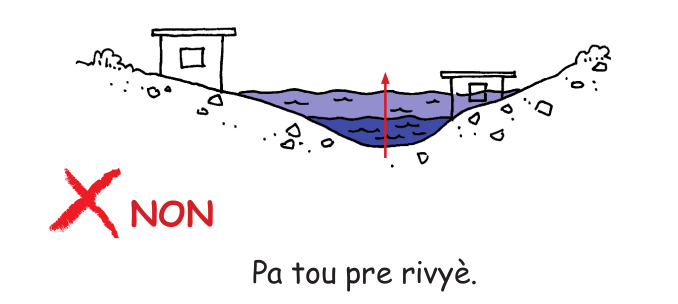
\includegraphics[width=\textwidth]{Pictures/KonstuiBoLarivye.png}
		\caption{Exemple d'illustration}
		\label{FigKonstuiBoRivye}
	\end{minipage}
	\begin{minipage}{0.5\textwidth}
		\centering
		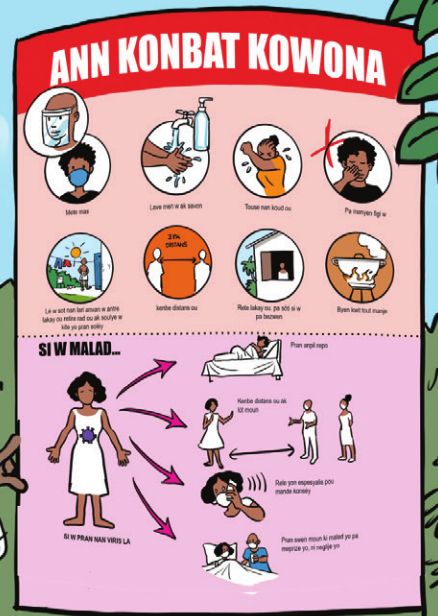
\includegraphics[height=0.3\textheight]{Pictures/AfichKontKowona.png}
		\caption{Affiche pour la sensibilisation contre le Covid-19}
		\label{LaveMenNouPouNouPaTrapeKowona}
	\end{minipage}
\end{figure}








\section{Avanc\'ees dans le domaine des syst\`emes d'information (SI)}
Suivant la probl\'ematique, nous devons construire un syst\`eme capable de rendre des fichiers num\'eriques accessibles.
% Le moyen le plus utilis\'e pour cela est d'entreposer les ressources \`a distribuer, et fournir l'acc\`es \`a cet entrep\^ot.
Un tel syst\`eme est appel\'e syst\`eme d'information.%\cite{DefinitionDeSI}\\


\noindent Un syst\`eme d'information permet de collecter des documents, de les stocker , de les traiter puis de les distribuer \`a la demande d'une personne tierce. Dans le cas o\`u les donn\'ees \`a manipuler sont des informations num\'eriques(fichiers ou donn\'ees), chacune des quatre fonctions du syst\`eme (collecter, stocker, traiter et communiquer) est assur\'ee par un ensemble de mat\'eriels informatiques, d'outils logiciels, de technologies et de proc\'edures. Le syst\`eme en soi sera r\'ealis\'e en connectant les diff\'erentes parties de mani\`ere \`a ce que l'ensemble puisse fournir une interface utilisateur ainsi que les services requis.

\subsection{Stockage de fichier dans le SI}
Le stockage d'information se r\'ef\`ere \`a la conservation de l'information. Cette t\^ache doit \^etre effectu\'ee de mani\`ere efficace, efficiente et s\'ecuris\'ee. En ce qui concerne le stockage d'information num\'erique, les avanc\'ees touchent notamment les supports sur lesquels les informations sont stock\'ees (les supports de stockage), les m\'ethodes permettant aux syst\`emes informatiques d'acc\'eder \`a l'espace de stockage (les solutions et technologies de stockage) et la forme sous laquelle les informations seront tra\^it\'ees.



\subsubsection{Supports de stockage}
Un p\'eriph\'erique de stockage est un composant \'electronique sur lequel on enregistre des donn\'ees num\'eriques. Il en existe plusieurs types (Carte SD, USB Flash Drive, Disque dur, etc.).\\
Chaque p\'eriph\'erique est caract\'eris\'e par sa volatilit\'e, sa capacit\'e de stockage, la vitesse \`a laquelle il peut lire ou \'ecrire des donn\'ees , la quantit\'e de donn\'ees qu'il peut transmettre par unit\'e de temps et la dur\'ee pendant laquelle il peut conserver des donn\'ees sans les alt\'erer.\\

\begin{itemize}
	\item[-] \textbf{La volatilit\'e} d\'ecrit le comportement du p\'eriph\'erique lorsqu'il est mis hors tension. Un p\'eriph\'erique est dit \emph{volatil} s'il perd les donn\'ees d\`es qu'il est mis hors tension, et \emph{non-volatil} si, dans le m\^eme cas, il les conserve pour un certain temps.\\
	\item[-] \textbf{La capacit\'e} d'un p\'eriph\'erique est la quantit\'e maximale de donn\'ees qu'il peut conserver. Elle est exprim\'ee en bytes (ou octet).
\end{itemize}



\paragraph{} \'Etant donn\'e que notre projet vise \`a stocker des informations de fa\c{c}on p\'erenne pour les distribuer ensuite. Les donn\'ees doivent n\'ecessairement \^etre stock\'ees sur des p\'eriph\'eriques non-volatils, de grande capacit\'e et avec une vitesse d'acc\`es ad\'equate. Ils doivent \'egalement offrir une vitesse de lecture raisonnable afin de limiter le temps de r\'eponse des requ\^etes effectu\'ees sur le syst\`eme et d'augmenter le nombre maximal d'acc\`es simultann\'es aux donn\'ees. \\
Parmi les p\'eriph\'eriques de stockage disponibles sur le march\'e, ceux qui r\'epondent \`a ces crit\`eres (non-volatil et de grande capacit\'e) sont d\'enomm\'es \emph{p\'eriph\'erique de stockage secondaire}\cite{stockagesSecondaire}. Les principaux sont les suivants.\\

\begin{itemize}
	\item[-] \textbf{P\'eriph\'erique de stockage magn\'etique}
	Le stockage magn\'etique utilise des bandes ou des disques recouverts d'un mince rev\^etement magn\'etique qui permet de conserver les donn\'ees sous forme de particules magn\'etique\cite{stockagesSecondaireMagnetique}. Le support le plus commun\'ement utilis\'e pour stocker des donn\'ees num\'eriques est  le disque dur(Hard disk Drive)\cite{stockagesSecondaireMagnetique}.\\

	\item[-] \textbf{P\'eriph\'erique de stockage SSD (Solid State Drive)\cite{stockagesSecondaire}}
	Le stockage SSD utilise des puces m\'emoires \'electroniques pour conserver les donn\'ees sous forme de charge \'electrique\cite{stockagesSecondaireElectrique}. Le p\'eriph\'erique SSD est tr\`es semblable au disque HDD. Les principales diff\'erences sont que: le SSD, utilise moins d'\'energie pour fonctionner, il est moins fragile, permet d'acc\'eder aux donn\'ees \`a une plus grande vitesse\cite{stockagesSecondaireElectrique}, et il est plus performant pour les acc\`es concurrentes en lecture ou en \'ecriture, bien qu'il ait une dur\'ee de vie moindre.\\

	\item[-] \textbf{RAID ( Redundant array of independent disks)\cite{MethodesEtTechnologies}\cite{MethodesEtTechnologies1}} \\
	Le RAID est une m\'ethode de stockage de donn\'ees qui consiste \`a utiliser plusieurs p\'eriph\'eriques de stockage ind\'ependants pour stocker les m\^emes donn\'ees. Avec cette m\'ethode, les donn\'ees sont organis\'ees de mani\`ere \`a ce que, si l'un des p\'eriph\'eriques tombe en panne, les autres suffisent pour reconstituer l'ensemble des donn\'ees que contenait le syst\`eme avant la panne. \par
	\noindent Le RAID permet de construire un syst\`eme tol\'erant aux pannes. Cette m\'ethode augmente la performance et la fiabilit\'e du syst\`eme de stockage.\\
\end{itemize}



\subsubsection{Solutions et technologies de stockage}
Au fil du temps, le fait de conserver les donn\'ees, en soi, s'est av\'er\'e insuffisant pour un stockage efficace et efficient. Il est devenu tout aussi important d'assurer la disponibilit\'e des donn\'ees, d'y bloquer l'acc\`es non-authoris\'e, de prot\'eger les syst\`emes contre les pannes et d'autres al\'eas. Ainsi de nombreuses m\'ethodes et technologies ont \'et\'e d\'evelopp\'ees pour aider \`a la conception, la gestion et la maintenance des syst\`emes de stockage. Chaque m\'ethode ou technologie est caract\'eris\'ee par un ensemble d'avantages et de contraintes, et ce sont ces caract\'eristiques qui serviront de base pour choisir quels moyens de stockage \`a adopter.\\

\begin{itemize}
	\item[-] \textbf{P\'eriph\'erique attach\'e\cite{MethodesEtTechnologies}\cite{MethodesEtTechnologies1}}\\
	C'est la m\'ethode utilis\'ee par d\'efaut pour fournir de l'espace de stockage aux ordinateurs. Elle consiste \`a attacher le p\'eriph\'erique de stockage directement \`a un ordinateur (PC, Desktop, Serveur). Cette m\'ethode permet d'allouer toute l'espace de stockage d'un p\'eriph\'erique \`a un seul ordinateur. Elle est la moins co\^uteuse, et offre une bonne performance. Mais elle est peu tol\'erante aux pannes. \\

	\item[-] \textbf{NAS (Network Attached Storage)}\\
	Cette m\'ethode consiste \`a d\'eployer un syst\`eme de stockage sous forme de serveur sur un r\'eseau. Ce syst\`eme fournit le stockage aux clients du r\'eseau comme un service. Les clients acc\`edent \`a ce syst\`eme de stockage via son addresse IP. \\

	\item[-] \textbf{SAN (Storage Area Network)\cite{MethodesEtTechnologies}\cite{MethodesEtTechnologies1}} \\
	Cette m\'ethode consiste \`a regrouper plusieurs p\'eriph\'eriques de stockage, de m\^eme type ou de types diff\'erents, en un seul grand syst\`eme de stockage qui servira d'espace de stockage \`a un ensemble de ressources informatiques. Cette solution offre une tr\`es grande performance et une haute disponibilit\'e des donn\'ees mais, elle est \'egalement tr\`es co\^uteuse.\\

	\item[-] \textbf{Stockage en nuage (Storage As A Service)\cite{MethodesEtTechnologies}\cite{MethodesEtTechnologies1}} \\
	Il s'agit de louer de l'espace de stockage aupr\`es d'un fournisseur. Le client peut acc\'eder \`a ses donn\'ees via Internet. Cette m\'ethode permet de se passer des co\^uts de d\'eploiement d'un syst\`eme de stockage local et de g\'erer les grandes fluctuations dans l'espace de stockage utilis\'e, en ne payant que pour ce qui est effectivement consomm\'e.\\

\end{itemize}

\subsubsection{Logiciels pour le stockage\cite{systemDeFichiers}\cite{UitiliteDesBaseDeDonnees}}
	Les informations num\'eriques peuvent \^etre stock\'ees soit sous forme de donn\'ees, soit sous forme de fichiers. \textit{Une donn\'ee est un fait observ\'e mais pas encore interpr\'et\'e}. Une fois interpr\'et\'ee, la donn\'ee devient une information. \textit{Un fichier est une collection structur\'ee de donn\'ees concernant un m\^eme sujet, r\'eunie sous un m\^eme nom}.



	\paragraph{} \textbf{Syst\`eme de fichiers}\\
	Un syst\`eme de fichiers fournit un environnement dans lequel des fichiers peuvent \^etre tra\^it\'es. Il est compos\'e d'un ensemble de fichiers et d'une structure de dossiers qui organise ces fichiers et fournit des informations sur chacun d'eux. Les ordinateurs sont g\'en\'eralement \'equip\'e d'un syst\`eme de fichiers built-in et d'un logiciel permettant de le g\'erer. Toutefois il est possible d'en programmer d'autres si n\'ecessaire.\\
	Cette m\'ethode est tr\`es efficace pour tra\^iter des informations sous forme de fichiers, mais elle s'est av\'er\'ee inefficace et non-adapt\'e \`a l'utilisation et la gestion de donn\'ees\cite{systemDeFichiers}. D'o\`u l'int\'er\^et des bases de donn\'ees\cite{DefinitionDeFichier2}.




	\paragraph{}\textbf{Base de donn\'ees}\\
	Une base de donn\'ees est une structure informatique qui sert \`a contenir une collection de donn\'ees et permet de les exploiter\cite{BaseDeDonnees}.
	Pour cr\'eer et/ou utiliser une base de donn\'ees, il est n\'ecessaire d'utiliser un Syst\`eme de Gestion de Base de Donn\'ees (SGBD). Il en existe plusieurs, tels que: Microsoft Access, MySQL, Oracle Database, OrientDB ou CouchDB.




	\subsection{Collecte, traitement et distribution des fichiers}
	En r\'eponse \`a la probl\'ematique, notre syst\`eme doit \^etre capable de transmettre des fichiers vers un maximum de personnes. Puisqu'il s'agit de fichiers num\'eriques, chaque personne doit disposer d'un syst\`eme informatique (Laptop, Desktop, Smartphone, tablette, etc.). Pour qu'un syst\`eme informatique puisse communiquer avec un autre, il doit s'interfacer (se mettre en r\'eseau) avec les syst\`emes avec lesquels il souhaite \'echanger des informations . Nous devons donc mettre notre syst\`eme en r\'eseau. Puisque nous voulons communiquer avec un maximum de personnes, nous devons utiliser Internet, qui est le plus grand des r\'eseaux informatiques. \\
	Nous devons donc d\'evelopper un syst\`eme d'information num\'erique accessible via Internet. Un moyen de faire cela est de construire une application web\cite{ApplicationWeb} qui fournit le service de transfert de fichiers.\\

\paragraph{} Dans une application web, la collecte et le traitement de fichiers sont impl\'ement\'es comme des services. Ces fonctions sont r\'ealis\'es par les  proc\'edures d'une application serveur.\\
Les avanc\'es, en ce qui concerne la cr\'eation de services dans une application web concernent notamment le langage de programmation et les frameworks utilis\'es. (\cite{techstack})

\subsubsection{Technologies de d\'eveloppement}
%			Comme nous venons de le voir, le syst\`eme d'information doit \^etre impl\'ement\'e \`a travers
Une application web est un programme informatique accessible via un navigateur\cite{ApplicationWeb}. Le d\'eveloppement d'une application web requiert l'utilisation de langage de programmation et d'autres outils et technologies utilis\'es dans la programmation.\\

\begin{itemize}
	\item[-] Interface utilisateur (Front-End)\cite{frontendprogramming}\\
	Pour d\'evelopper l'interface utilisateur, on peut utiliser HTML, CSS et JavaScript, ou opter pour un framework bas\'e sur ces langages comme Angular, Vue ou React.
	\item[-] D\'eveloppement c\^ot\'e serveur (Back-End)\cite{backendprogramming}\\
	L'impl\'ementation des fonctions (collecte, traitement et distribution), requiert de coder les proc\'edures qui vont fournir les services n\'ecessaires et utiliser des requ\^etes pour communiquer avec la base de donn\'ees. Pour cela, il faut utiliser un langage de programmation tel que PHP, Python, Ruby, Java ou C\#. Il faudra ensuite choisir un framework bas\'e sur le langage s\'electionn\'e. Parmi les framework fr\'equemment utilis\'es, on peut citer: Express, Spring, Django, Laravel, Rails, et .NET.
	\item[-] Base de donn\'ees\\
	Pour construire une base de donn\'ees, nous devons d'abord choisir un syst\`eme de gestion de base de donn\'ees suivant les besoins de l'application. Il en existe beaucoup. Parmi les plus connus: MySQL, PostgreSQL, MongoDB, MariaDB, etc.\\
	Ensuite, il faut cr\'eer un mod\`ele de donn\'ees qui servira de base pour \'elaborer le sch\'ema des donn\'ees en utilisant le langage du SGBD choisi.


\end{itemize}






\section{L'illustration en Ha\"iti et dans le monde}
\label{SectionAvantageIllustrations}
L'illustration, telle que d\'efinie dans l'introduction, est omnipr\'esente dans la vie quotidienne. On la retrouve dans des r\'ecits oraux, des livres, les journaux, les magazines, les affiches, les bandes dessin\'ees, les jeux vid\'eo, les films d'animation, etc. \\
Suivant le format de document num\'erique utilis\'e, une illustration peut \^etre une image, un texte, un fichier audio ou un fichier vid\'eo.


\subsection{Importance de l'illustration}
Le fait d'utiliser des illustrations pr\'esente plusieurs avantages. Voici une liste non-exhaustive de leurs traits b\'en\'efiques qui pourraient \^etre exploit\'es dans notre syst\`eme.

\subsubsection{Expliquer simplement}
Les illustrations permettent d'expliquer facilement des concepts qui pourraient \^etre complexes et difficiles \`a comprendre \`a travers des expos\'es explicatifs classiques. Des illustrations sont utilis\'ees \`a cet effet dans des  livres, des articles, des sites Web, etc. La figure~\ref{CiscoReseau} montre un cas o\`u le concept de transfert de message est illustr\'e dans le livre `` CCNP and CCIE Enterprise Core `` de Cisco.


\begin{figure}[ht]
	\centering
	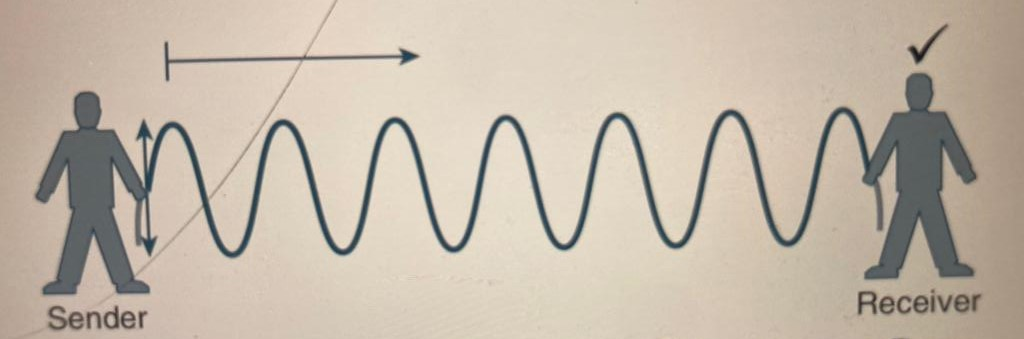
\includegraphics[width=0.75\linewidth]{Pictures/Sending Message.jpg}
	\caption{Illustration d'un transfert de message\cite{CiscoMessage}}
	\label{CiscoReseau}
\end{figure}


\subsubsection{Susciter l'engagement du spectateur}
Les illustrations peuvent rendre des contenus beaucoup plus engageant en cr\'eant un contexte dans lequel le spectateur peut s'identifier pleinement. Par exemple, elles sont utilis\'ees dans les livres pour enfants, pour les garder engag\'es dans la lecture et stimuler leur int\'er\^et pour la lecture comme dans ''The three questions'' by Jon J. Muth. De m\^eme, dans la vid\'eo illustr\'ee intitul\'ee ''Ey chof\`e, P\`otay ou prale?'' utilis\'ee par la T\'el\'evision Nationale d'Ha\"iti (TNH) pour sensibiliser la population \`a respecter les feux de signalisation sur les routes. Le contexte, notamment, la destination du personnage (Portail L\'eoganne), les camionnettes, les intervenants, le d\'ecor en g\'en\'eral, rappelle l'environnement ha\"itien et incite un ha\"itien qui regarde la vid\'eo \`a se sentir concern\'e par le contenu.\\


\subsubsection{Faciliter la m\'emorisation du contenu}
La m\'emorisation est le fait de conserver des informations pour pouvoir s'en rappeler apr\`es un certains temps. De nombreux facteurs  internes ou externes (attention, sant\'e, alimentation, hygi\`ene de vie, fr\'equence \`a laquelle nous acc\'edons \`a l'information, la valeur \'emotionnelle qu'on lui accorde ) peuvent affecter la m\'emorisation d'une information soit en la facilitant, soit en la rendant plus compliqu\'ee.  Les illustrations peuvent \^etre utilis\'ees pour faciliter la m\'emorisation :\\

\begin{itemize}
	\item[-] Dans une illustration, chaque \'el\'ement d'information est situ\'e dans un contexte bien d\'efini, de sorte qu'il puisse \^etre li\'e aux autres informations constituant l'illustration. \cite{ContextDependencyEffect}
	\item[-] Les illustrations graphiques et vid\'eos offrent une repr\'esentation visuelle directe, ce qui rend les informations plus faciles \`a retenir. \cite{ImageMemoire} \cite{ImageMemoireb}
	\item[-] Certaines illustrations repr\'esentent des r\'ecits narratifs dans lesquels l'information utile est introduite. Cette approche narrative rend le contenu plus facile \`a m\'emoriser.\cite{NarrationMemoire}
\end{itemize}
Par cons\'equent, L'utilisation d'illustrations augmente les chances que les personnes qui visionnent les documents se souviennent des informations re\c{c}ues.


\subsection{Utilisations faites des illustrations}


\subsubsection{Attirer l'attention}
Des illustrations tr\`es color\'ees sont utilis\'ees pour inciter les gens \`a pr\^eter attention au contenu. Elles sont souvent employ\'ees dans les livres pour enfant (Comme Le petit prince de \cite{LePetitPrince}) ou en marketing comme le montre l'affiche publicitaire de la figure~\ref{FigMaltaH}.



\begin{figure}[ht]
	\centering
	
\includegraphics[width=0.50\linewidth]{Pictures/MaltaH.jpg}
	\caption{Affiche publicitaire illustr\'ee visant \`a attirer l'attention}
	\label{FigMaltaH}
\end{figure}



\subsubsection{Rendre des informations plus accessibles}
Les illustrations sont utilis\'ees pour rendre des informations plus accessibles. Elles permettent de communiquer avec les personnes atteintes de c\'ecit\'e ou de troubles auditifs, pourvu qu'elles disposent de l'un ou l'autre de ces sens, l'ou\"ie et la vue. Elles ne requi\`erent pas beaucoup de temps pour transmettre le message, ce qui est avantageux pour ceux qui n'ont pas beaucoup de temps pour s'informer. Certaines illustrations utilisent une forme d'expression intuitive ne n\'ecessitant pas de connaissances sp\'ecifiques pour \^etre interpr\'et\'ees. Ainsi elles permettent de communiquer efficacement notamment avec les enfants, mais aussi avec les membres de la communaut\'e qui sont analphab\`etes (soit plus de 48\% de la population locale  en 2018\cite{AnalphabetismeHaiti}) ou qui pr\'esentent certains autres formes de limitation intellectuelle.

\subsubsection{Communiquer}
Les illustrations sont utilis\'ees pour communiquer des messages. Notamment pour faire face \`a une \'epid\'emie (Voir Figure~\ref{FigCovid}), une catastrophe naturelle (Voir Figure~\ref{ConsigneSeisme}) ou pour s'adresser aux enfants (Voir Figure~\ref{ConsigneToillette}), on en fait souvent usage. Elles sont aussi tr\`es utilis\'ees pour faire passer des avertissements (Voir Figure~\ref{Avertissement}).

	\begin{figure}[ht]
		\vspace{10pt}
		\centering
		\begin{minipage}{0.45\textwidth}
			\centering
			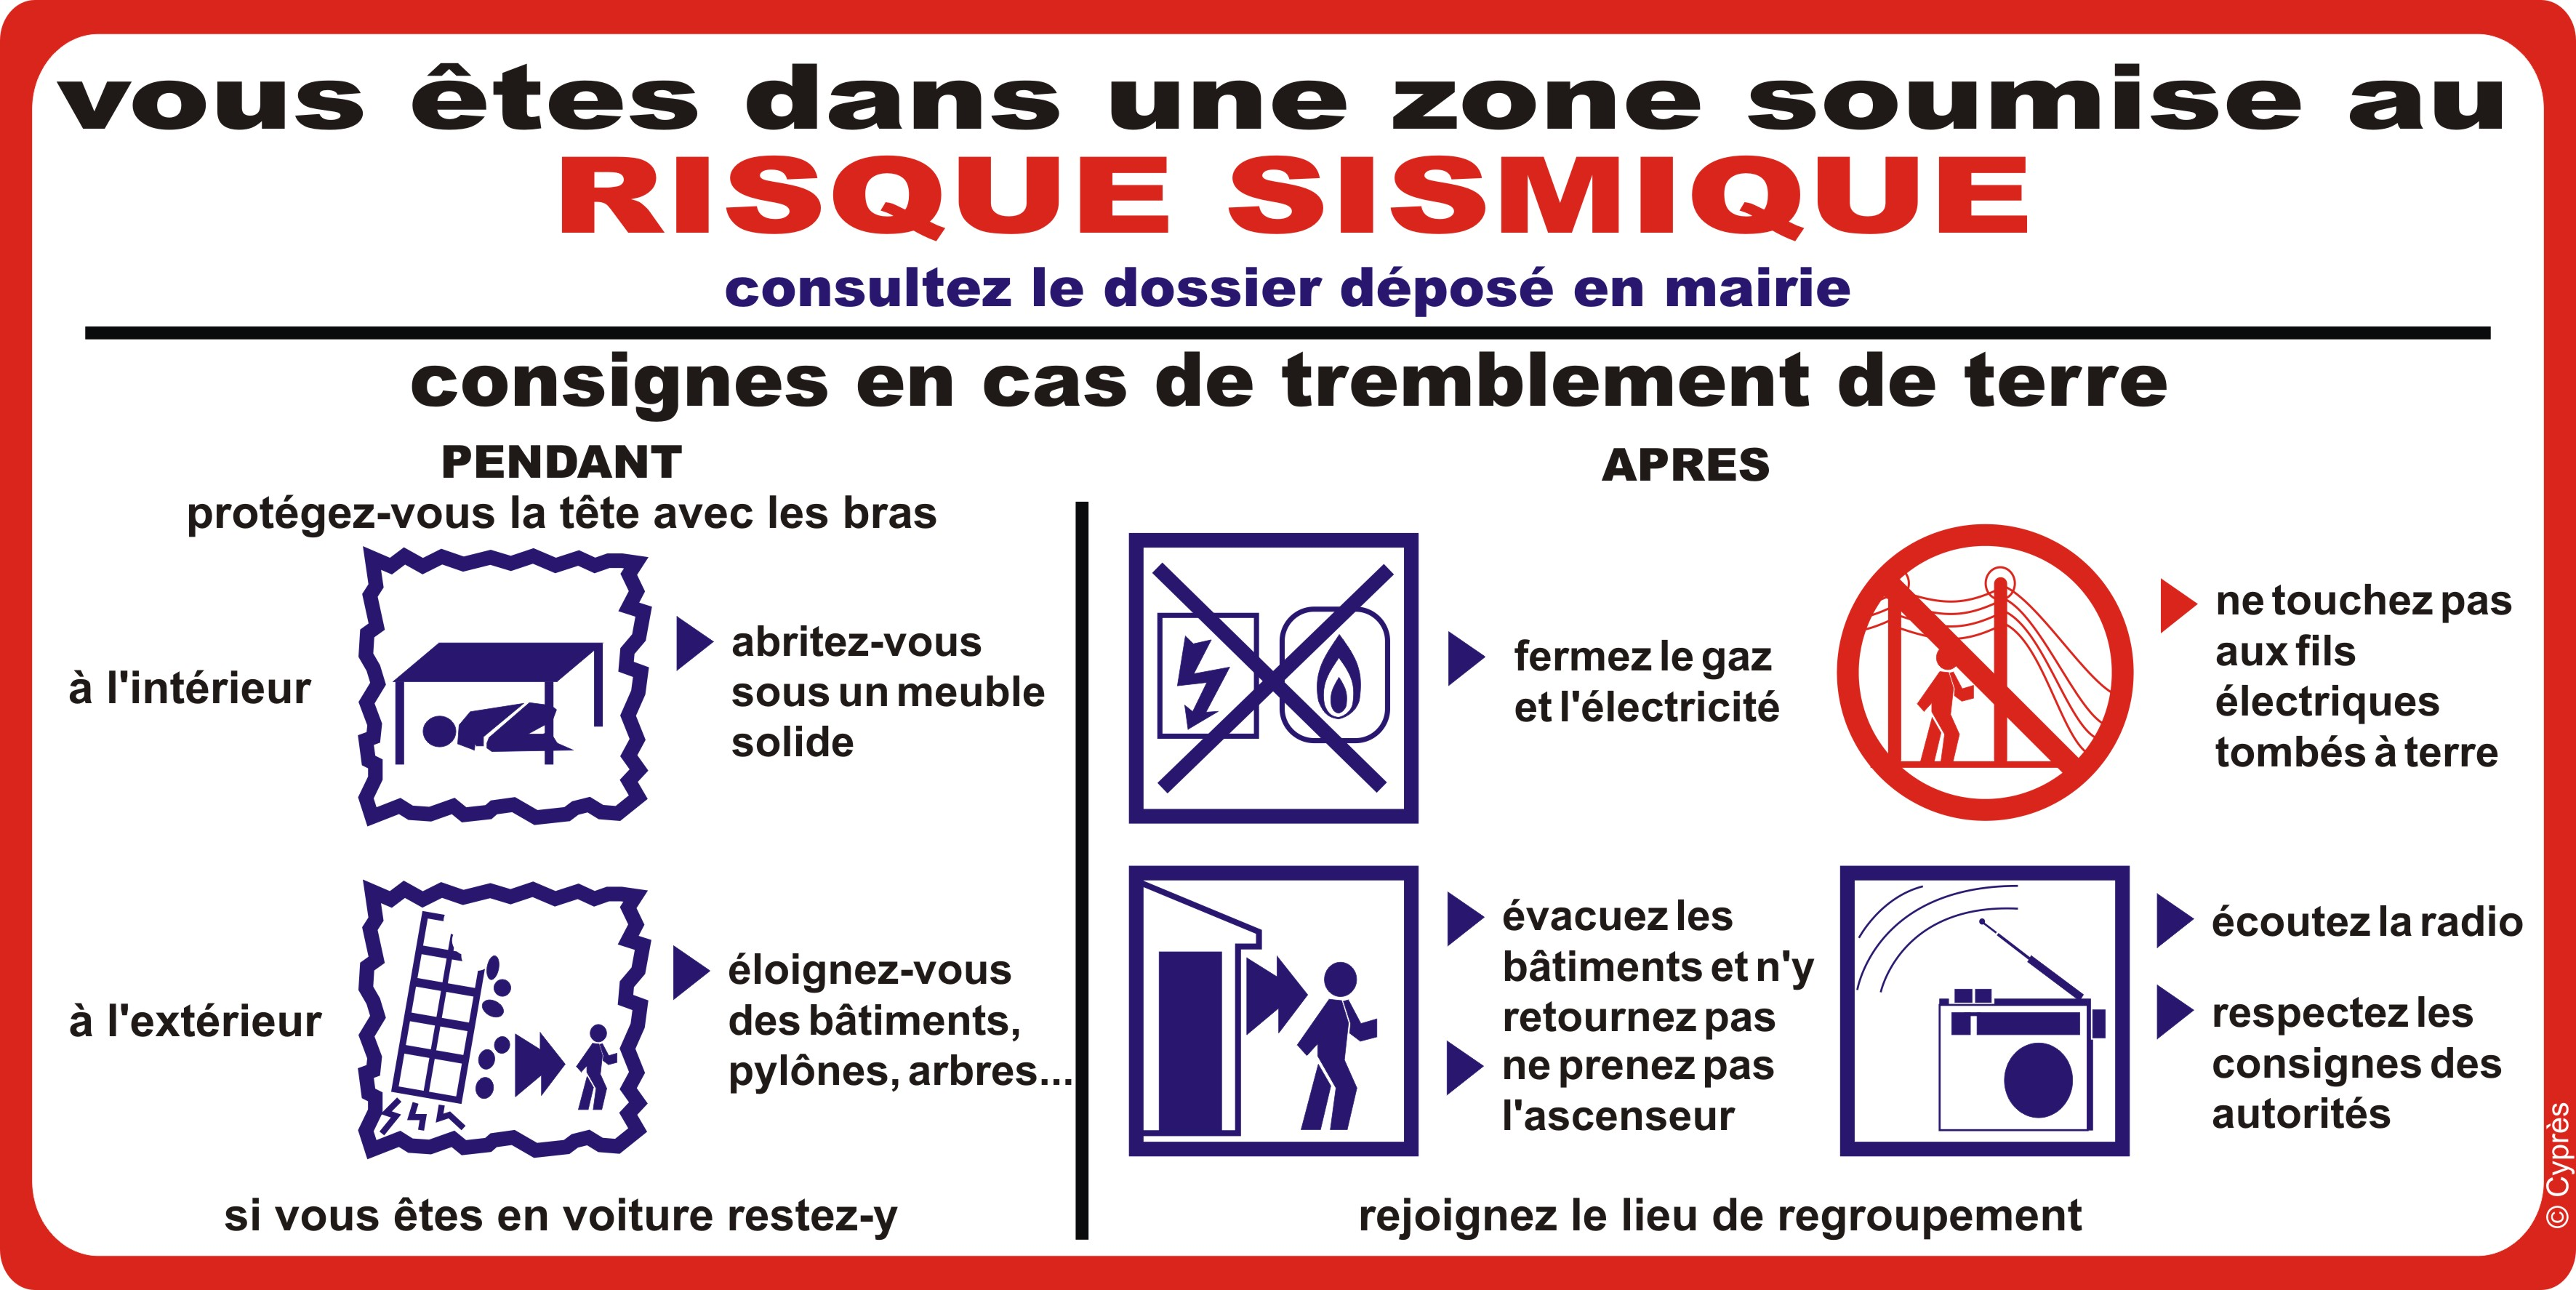
\includegraphics[width=5cm]{Pictures/RisqueSismique.jpg}
			\caption{Illustration des consignes pour se prot\'eger pendant et apr\`es un s\'e\"isme}
			\label{ConsigneSeisme}
		\end{minipage}
		\hspace{10pt}
		\begin{minipage}{0.45\textwidth}
			\centering
			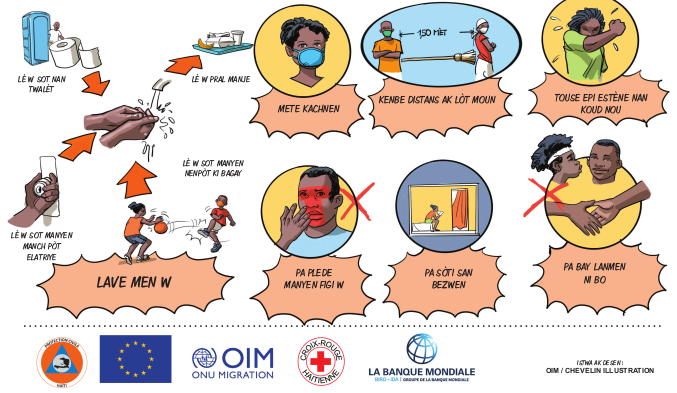
\includegraphics[width=5cm]{Pictures/FigCovid.png}
			\caption{Illustration des consignes pour se prot\'eger contre le Covid-19}
			\label{FigCovid}
		\end{minipage}

		\vspace{10pt}

		\begin{minipage}{0.45\textwidth}
			\centering
			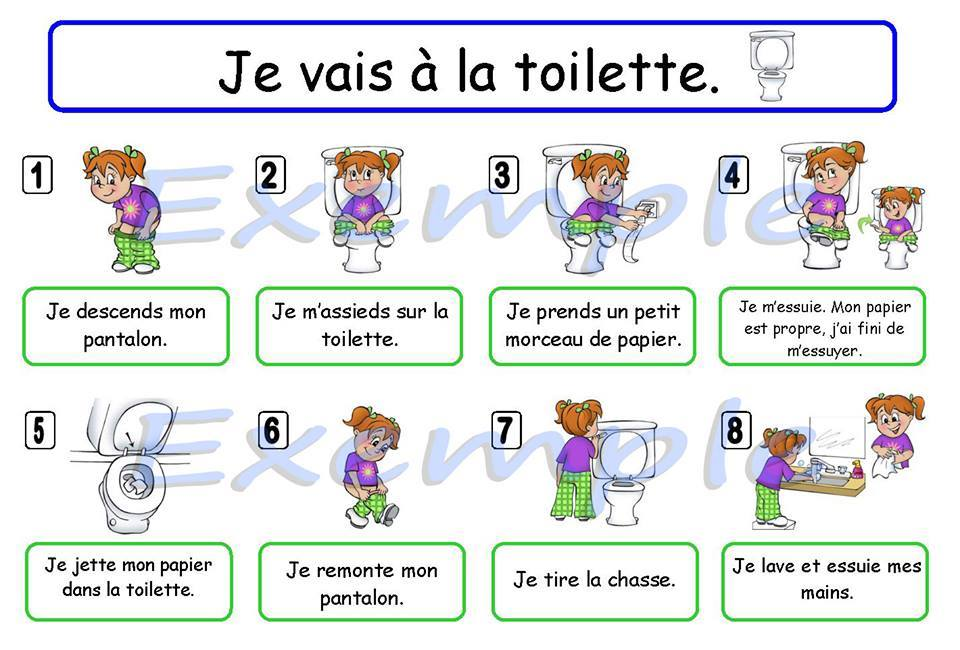
\includegraphics[width=5cm]{Pictures/SeServirDeLaToilettePourEnfant.jpg}
			\caption{Illustration enseignant aux enfants comment se servir des toilettes}
			\label{ConsigneToillette}
		\end{minipage}
		\hspace{10pt}
		\begin{minipage}{0.45\textwidth}
			\centering
			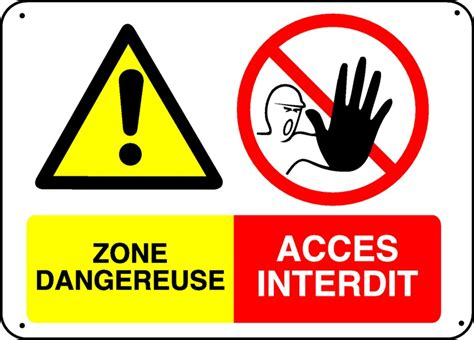
\includegraphics[width=5cm]{Pictures/Avertissement.jpg}
			\caption{Illustration permettant d'avertir les gens}
			\label{Avertissement}
		\end{minipage}
	\end{figure}


\subsubsection{Identifier une entit\'e}
Les illustrations, telles que les embl\`eme (voir figure~\ref{ArtOfWarGlobalConflict}), logos (voir figure~\ref{BrasserieDeLaCouronne}) ou slogans (voir figure~\ref{Petrochallengers}), sont utilis\'ees pour identifier des groupes d'individu (des pays, \'equipes de sports, ...), des mouvements sociaux (La r\'evolution russe, Les p\'etrochallengers\cite{PetroChallenger, PetroChallenger1}, ...) ou des marques.




\begin{figure}[ht]
	\vspace{10pt}
	\centering
	\begin{minipage}{0.45\textwidth}
		\centering
		
\includegraphics[width=5cm]{Pictures/ArtOfWar3.jpg}
		\caption{Embl\`eme des deux factions du jeu Art of war 3 - Global conflict }
		\label{ArtOfWarGlobalConflict}
	\end{minipage}
	\hspace{10pt}
	\begin{minipage}{0.45\textwidth}
		\centering
		
\includegraphics[width=5cm]{Pictures/BrasserieDeCouronneLogo.jpeg}
		\caption{Logo de la compagnie Brasserie de la couronne. \textbf{Source}: \href{https://www.linkedin.com/company/bracour/?originalSubdomain=ht}{Brasserie de la Couronne S.A.} }
		\label{BrasserieDeLaCouronne}
	\end{minipage}

	\vspace{10pt}

	\begin{minipage}{0.45\textwidth}
		\centering
		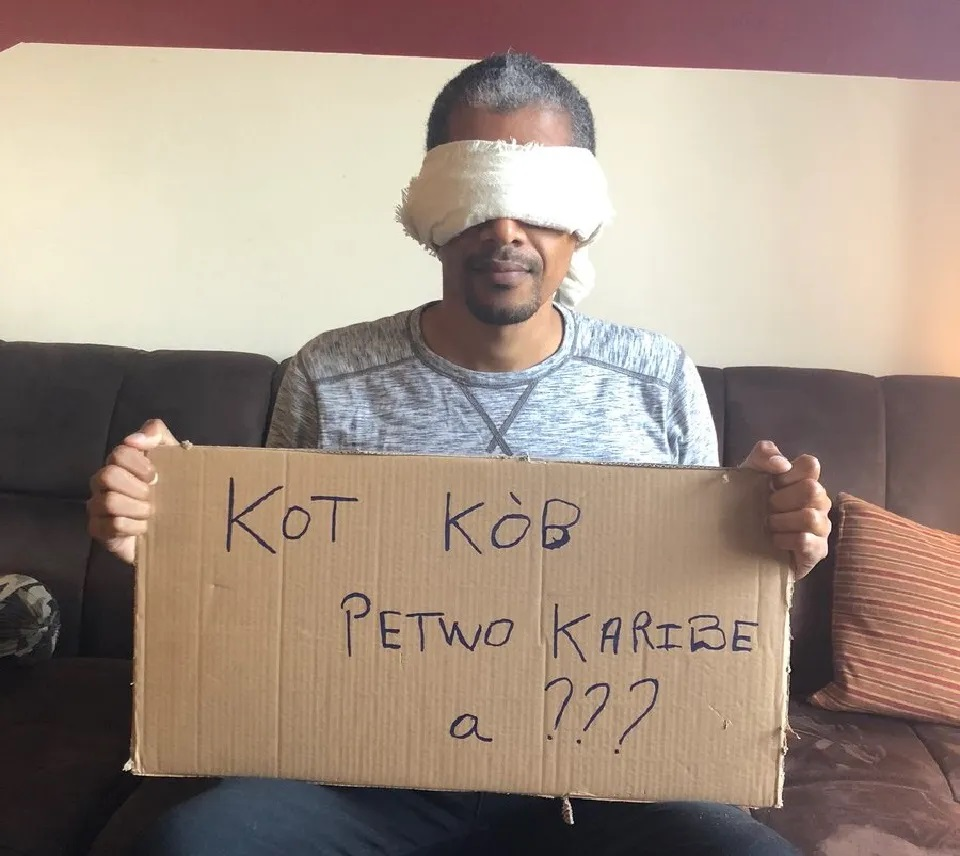
\includegraphics[height=5cm]{Pictures/PetroChallengerSlogan.jpg}
		\caption{Slogan du mouvement social ha\"itien Petro-Challengers\cite{PetroChallenger}}
		\label{Petrochallengers}
	\end{minipage}
	\hspace{10pt}
	\begin{minipage}{0.45\textwidth}
		\centering
		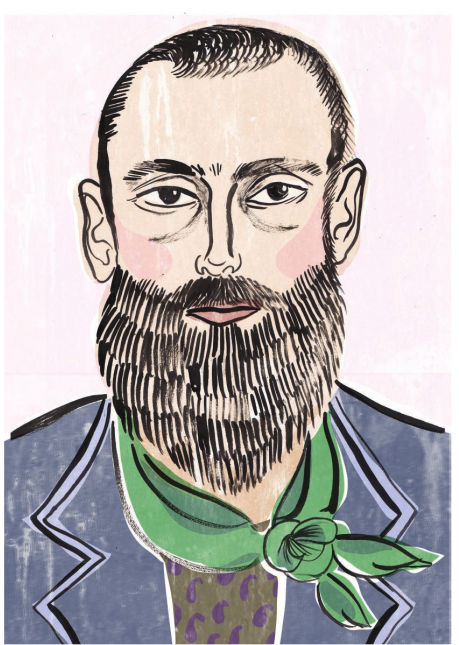
\includegraphics[height=5cm]{Pictures/IllustrationCommeArt.png}
		\caption{Image d'une illustration artistique\cite{ArtIllustre}}
		\label{IllustrationArt}
	\end{minipage}
\end{figure}

\subsubsection{Aide \`a la compr\'ehension}
Il s'agit l\`a de l'une des utilisations les plus r\'epandues des illustrations. Dans les livres, les articles, les sites internet et autres, les explications textuelles sont souvent accompagn\'ees d'illustrations graphiques pour offrir une expression plus claire des explications d\'ej\`a donn\'ees sous forme de texte (Voir Figure~\ref{CiscoReseau}).

\subsubsection{Art}
Les illustrations sont aussi utilis\'ees dans le domaine des arts, telle une fa\c{c}on cr\'eative, esth\'etique d'exprimer des id\'ees.(Voir figure~\ref{IllustrationArt}).


\section{Projets Similaires}
	Que ce soit pour Ha\"iti ou ailleurs, nous n'avons pas trouv\'e de projet ayant exactement le m\^eme objectif que le n\^otre: cr\'eer un syst\`eme d'information pour distribuer des illustrations afin de communiquer des informations sur les risques dans une r\'egion donn\'ee. Cependant, nous avons trouv\'e des projets qui abordent des aspects similaires. Pour ce document, nous nous proposons d'\'etudier trois groupes de projets suivant qu'ils consistent \`a cr\'eer un syst\`eme d'information pour pouvoir distribuer des documents via Internet, exploiter des illustrations dans un sens g\'en\'eral ou s'en servir pour enseigner.


	\subsection{Groupe 1 - Librairies en ligne}
		Une librairie en ligne est un site Internet qui fournit l'acc\`es \`a une collection de livres, articles, magazine, fichiers audio, images ou tout autre type de document accessible en ligne. Ces librairies peuvent offrir diff\'erents types de services notamment Le t\'el\'echargement, la lecture en ligne (streaming) ou le pr\^et (acc\`es pour une p\'eriode limit\'ee). Il existe beaucoup de librairie en ligne: Open Library, Europeana, Digital Public Library of America, The Online Books Page, Manybooks pour ne citer que quelques-unes. Elles se distinguent, entre autres, par la source des contenus propos\'es, leur public cible, les types de contenu propos\'e, les sujets couverts, le co\^ut d'acc\`es aux contenus ou leur politique d'utilisation et de redistribution des contenus. \`A titre d'exemple, nous pr\'esentons les d\'etails du projet Open Library.

		\subsubsection{Open Library}
			Open Library est un projet de Internet Archive\cite{InternetArchive} visant \`a rendre tous les livres accessibles \`a tous\cite{OpenLibVision}. C'est une librairie en ligne open source.\\

			\begin{itemize}
				\item[-] \textbf{Source des contenus}\\
				Les livres sur Open Library proviennent de sources divers, notamment, de partenariats, d'achats et de dons.\\

				\item[-] \textbf{Outils et technologies de d\'eploiement}\\
				Open library utilise Python comme langage de programmation, avec web.py comme framework ainsi qu'Infogami et Solr pour impl\'ementer certains services cot\'e serveur. Pour la base de donn\'ees, elle utilise PostgreSQL comme syst\`eme de gestion de base de donn\'ees et Memcached pour la gestion du cach. Cot\'e client, Open Library utilise Node.js pour la conception de l'interface web, Nginx pour g\'erer les requ\^etes des clients.\\

				\item[-] \textbf{Services offert}s\\
				Sur Open Library, vous pouvez lire un livre en ligne, l'\'ecouter, ou l'emprunter pour y acc\'eder hors ligne pendant une dur\'ee limit\'ee.\\

				\item[-] \textbf{Co\^uts et conditions d'acc\`es aux contenus}\\
				L'acc\`es aux livres est enti\`erement gratuit. Pour lire, \'ecouter, ou emprunter un livre, vous devez vous authentifier soit en cr\'eant un compte d'utilisateur ou en utilisant un compte Google.
			\end{itemize}





		\subsection{Groupe 2 - Projet de distribution d'illustrations}
			Une illustration \'etant avant tout un document, il est possible de trouver des illustrations dans toutes les librairies. De plus, il existe plusieurs sites web d\'edi\'es exclusivement \`a la distribution d'illustrations. Dont les suivants.\\

			\begin{itemize}
				\item[-] \textbf{Freepik}\\
					Freepik est une plateforme fond\'ee en 2010 par Alejandro Blanes, Pablo Blanes and Joaqu\'in Cuenca. Elle offre des illustrations de haute qualit\'e et propose une large gamme de ressources telles que des vid\'eos, des vecteurs, des photos, des maquettes, etc. Certaines de ces illustrations repr\'esentent des concepts li\'es \`a la gestion des risques comme \textbf{les s\'e\"isme, les temp\`ete, les catastrophes naturelles, etc} (Voir Figure~\ref{TempeteFromFreepik} et Figure~\ref{CatastropheNaturelleFromFreepik}). Freepik offre un acc\`es gratuit ainsi q'un acc\`es premium.\\

					\begin{figure}[ht]
						\vspace{10pt}
						\centering
						\begin{minipage}{0.45\textwidth}
							\centering
							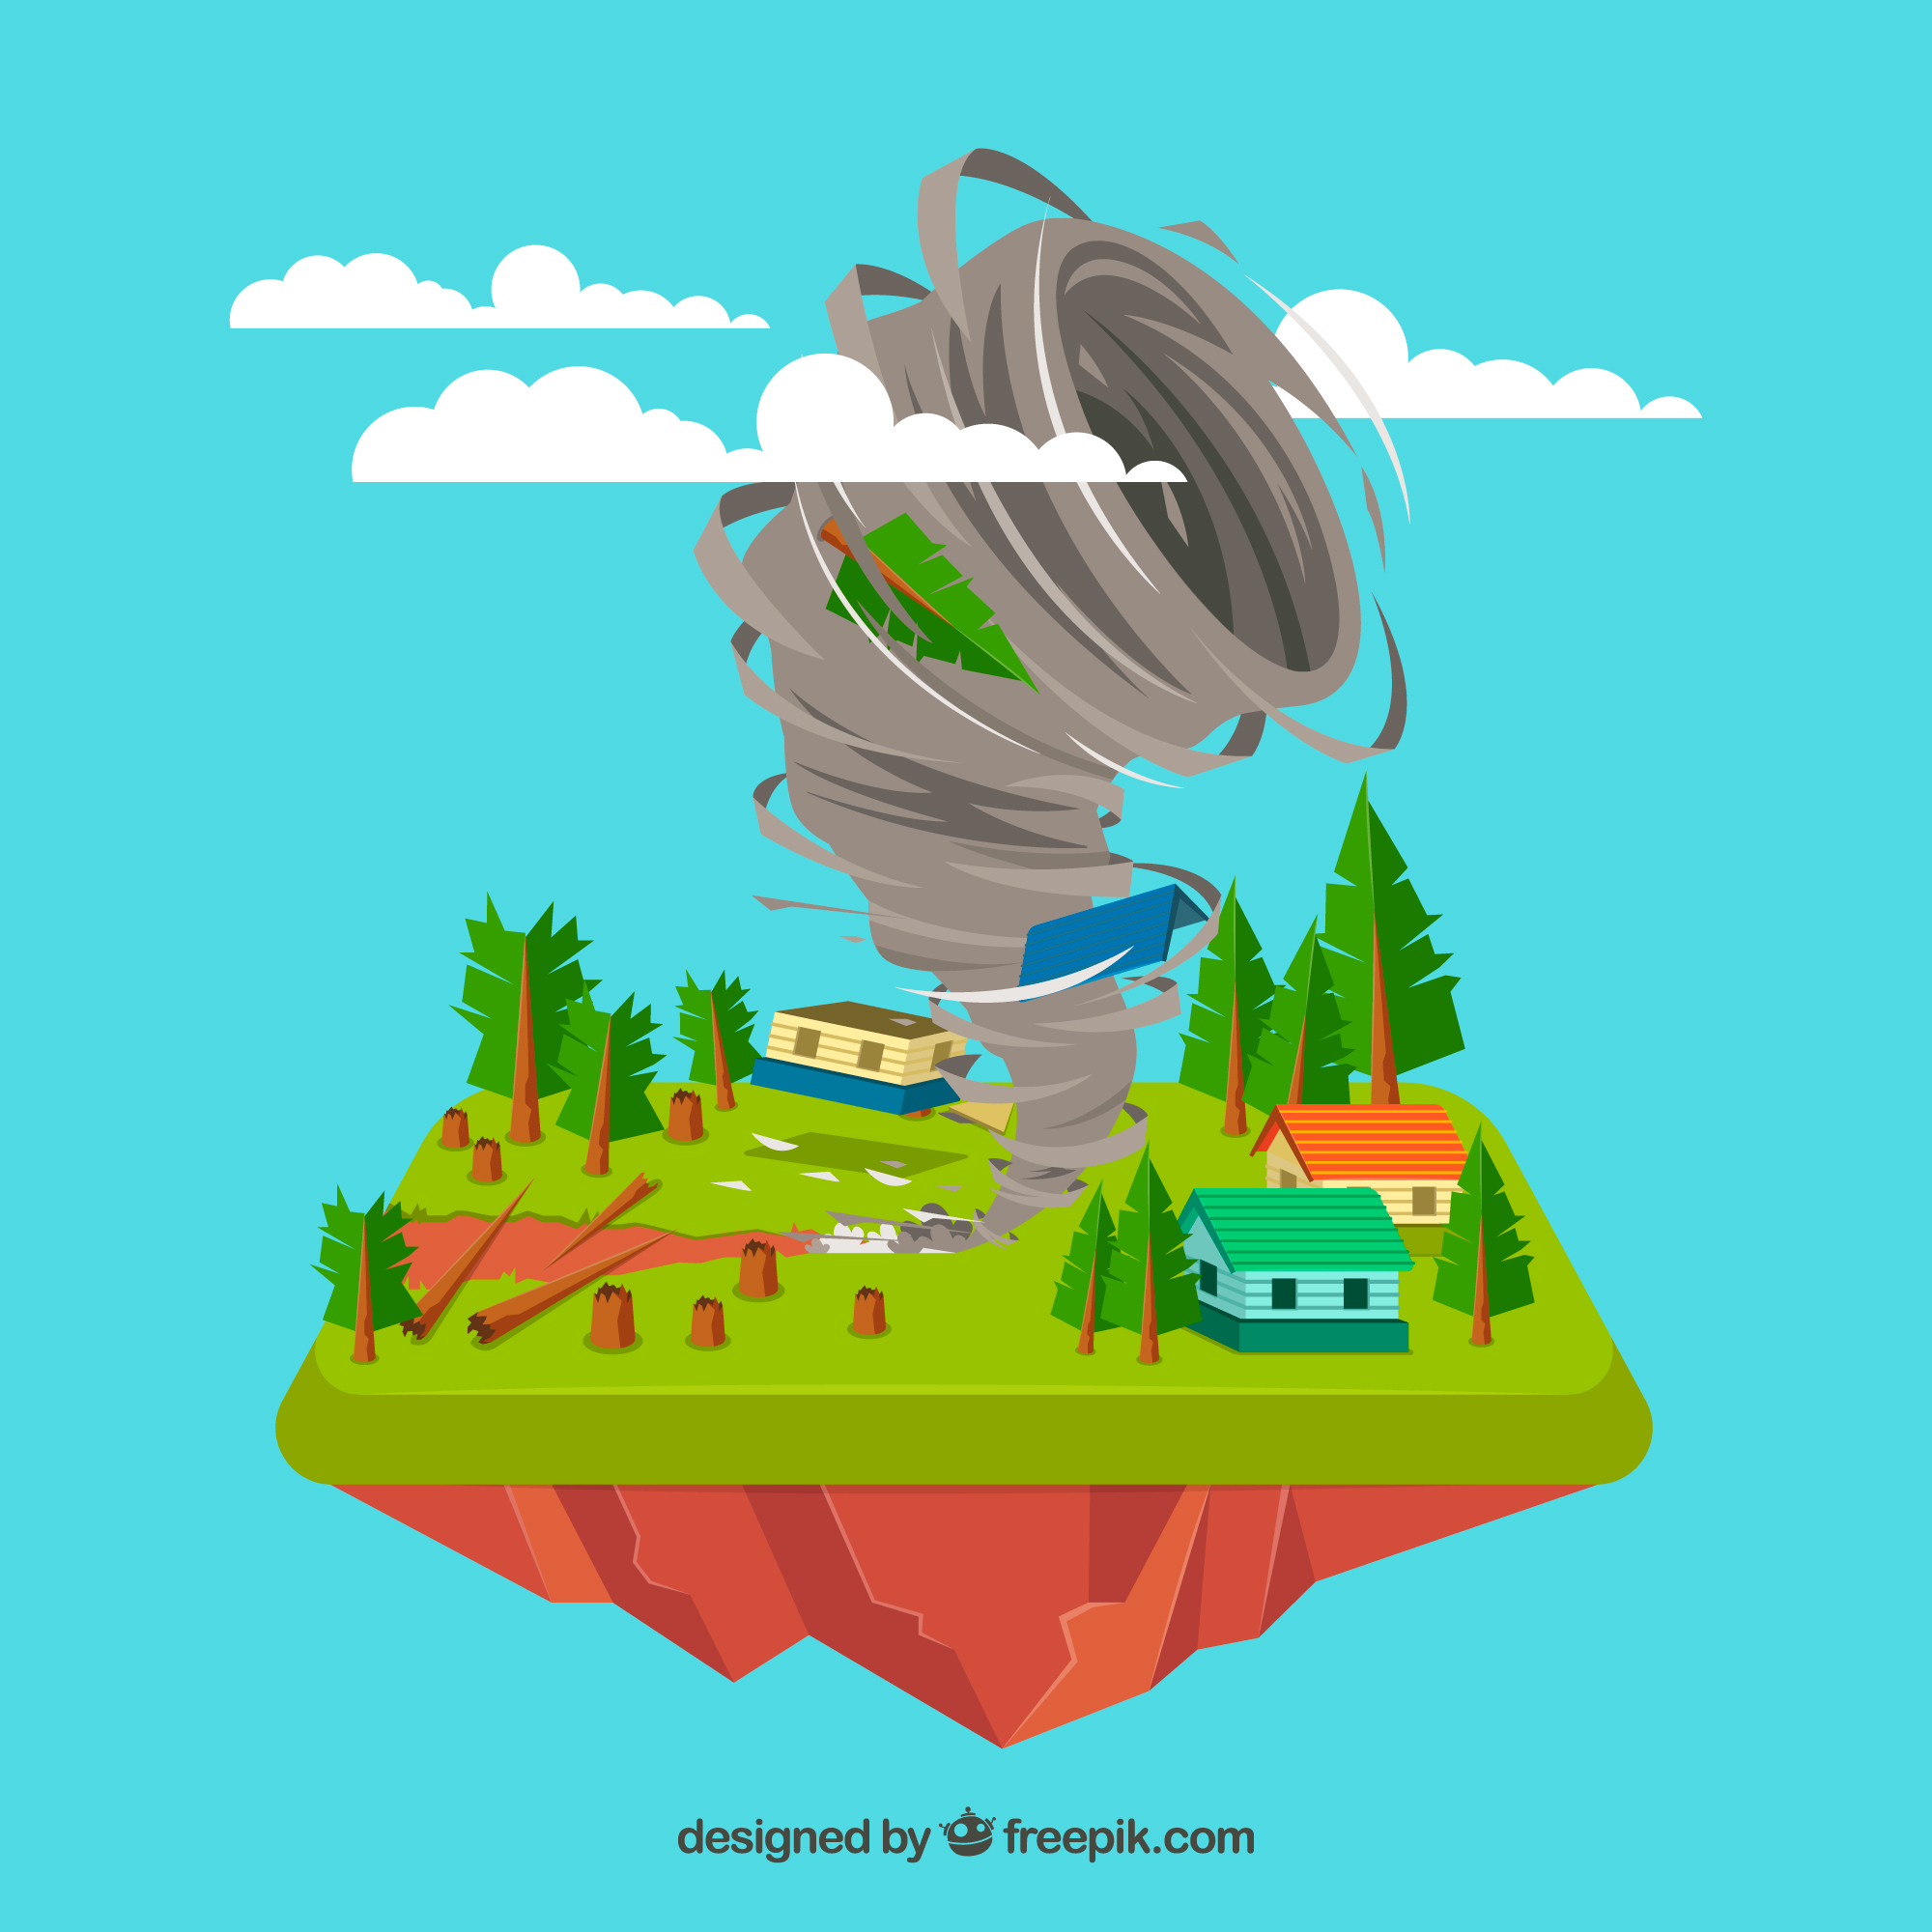
\includegraphics[width=5cm]{Pictures/CatastropheNaturelleFreepik.jpg}
							\caption{Illustration d'une catastrophe naturelle par \href{https://www.freepik.com/}{Freepik}}
							\label{CatastropheNaturelleFromFreepik}
						\end{minipage}
						\hspace{10pt}
						\begin{minipage}{0.45\textwidth}
							\centering
							
\includegraphics[width=5cm]{Pictures/TempeteFreepik.jpg}
							\caption{Illustration d'une temp\^ete par \href{https://www.freepik.com/}{Freepik}}
							\label{TempeteFromFreepik}
						\end{minipage}
					\end{figure}

				\item[-] \textbf{Pixabay}\\
					Pixabay est une plateforme de distribution d'illustrations gratuites sous licence libre. Elle fournit plus de 4 millions de vid\'eos, fichiers audio, images et autres m\'edias. On y trouve certains contenus qui concerne des concepts li\'es au risque.\\

				\item[-] \textbf{Craftwork}\\
					Craftwork Studio vous permet de commander des illustrations personnalis\'ees. Vous pouvez discuter avec eux de votre projet et des graphiques sp\'ecifiques dont vous aurez besoin. Ils cr\'eeront des \'ebauches initiales que vous pourrez examiner et commenter. Une fois le design affin\'e et parfait, vous recevrez votre design personnalis\'e.\\


				\item[-] \textbf{DesignCrowd}\\
					Sur DesignCrowd, vous pouvez lancer votre projet en leur indiquant ce dont vous avez besoin. Vous recevrez des propositions d'illustrations uniques du monde entier en quelques heures. Vous pouvez ensuite s\'electionner et approuver votre design pr\'ef\'er\'e et t\'el\'echarger les fichiers.


			\end{itemize}


		\paragraph{} De tous les projets que nous avons trouv\'e, le projet avec les objectif les plus proches du n\^otre en ce qui concerne les illustrations est \textbf{Kurzgesagt}.

\subsubsection{Kurzgesagt}
	Kurzgesagt est un studio d'animation allemand qui  vise \`a suciter la curiosit\'e de ses spectateurs et \`a encourager une vision du monde optimiste, bas\'ee sur la science et humaniste. Ainsi il travaille, entre autres, \`a produire des vid\'eos illustr\'es (graphes, animations, contexte narrative, ...) dans le but de vulgariser des connaissances scientifiques autour de sujets tels que la biologie, la physique, la chimie, l'\'economie ou l'astronomie en produisant notamment des videos illustr\'ees qu'il publient sur leurs cha\^ines YouTube. Les illustrations sont utilis\'ees pour rendre le contenu informatif amusant, esth\'etique et accessible \`a autant de gens que possible ind\'ependamment de leur \^age ou de leur formation acad\'emique.

	\begin{figure}[ht]
		\vspace{10pt}
		\centering
		\begin{minipage}{0.45\textwidth}
			\centering
			
\includegraphics[width=5cm]{Pictures/LogoKurzgesagt.png}
			\caption{Logo de \href{https://www.kurzgesagt.org/}{Kurzgesagt}}
			\label{LogoKurzgesagt}
		\end{minipage}
		\hspace{10pt}
		\begin{minipage}{0.45\textwidth}
			\centering
			
\includegraphics[width=7cm]{Pictures/AnimauxConnus.png}
			\caption{Image extraite de la vid\'eo \href{https://www.kurzgesagt.org/}{\textbf{\`A quoi ressemblaient VRAIMENT les dinosaures ?}} de Kurzgezagt.}
			\label{FigDino}
		\end{minipage}
	\end{figure}



\subsection{Groupe 3 - Utilisation des illustrations comme vecteur de communication}
Que ce soit sur les librairies qui distribuent des documents d'une fa\c{c}on g\'en\'erale ou parmi les projets qui se focalisent sur la distribution d'illustrations, nous trouvons des documents dans lesquels des illustrations sont utilis\'ees comme vecteur de communication. Dans cette cat\'egorie on retrouve les bandes d\'essin\'ees, les mangas comme moyen de communication, les livres pour enfant et bien d'autres ouvrages. La figure~\ref{FigDino} en est un exemple. Cette illustration repr\'esente nos connaissances sur les animaux tout en mettant l'emphase sur le fait le fait que certains nous sont encore inconnus.

\subsubsection{Alain Possible et le monde possible \cite{AlainPossible}}
Alain Possible et le Monde Possible est une s\'erie de bandes dessin\'ees publi\'ee par les Nations Unies dans le cadre d'une initiative soutenant les objectifs de d\'eveloppement durable en Ha\"iti. Le projet vise \`a sensibiliser les acteurs de la population locale aux objectifs de d\'eveloppement durable. Dans cette bande d\'essin\'ee, les illustrations sont utilis\'ees pour communiquer avec la population locale sur la signification du concept de d\'eveloppement durable, son importance, et les \'eventuels d\'eg\^ats que pourraient causer l'absence de sa prise en compte dans les projets \'etatiques (Voir Figure~\ref{TheTimeMachin}).




\begin{figure}[ht]
	\vspace{10pt}
	\centering
	\begin{minipage}{0.45\textwidth}
		\centering
		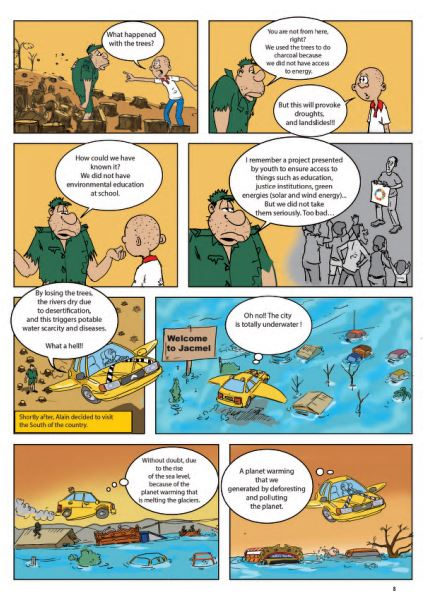
\includegraphics[width=5cm]{Pictures/AlainPossibleTheTimeMachine.jpg}
		\caption{Alain possible et le monde possible - La machine du temps / Page 8\cite{AlainPossible}}
		\label{TheTimeMachin}
	\end{minipage}
	\hspace{10pt}
	\begin{minipage}{0.45\textwidth}
		\centering
		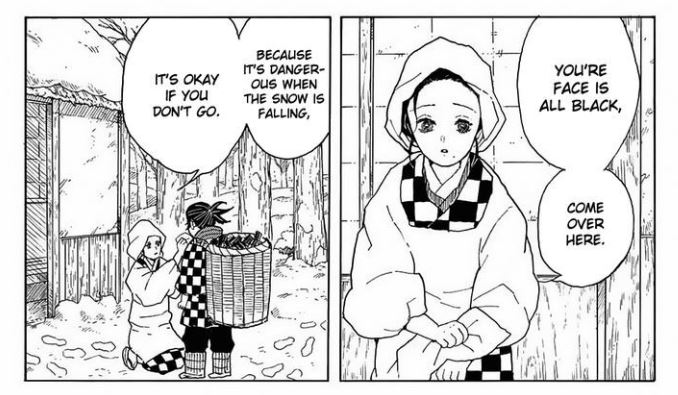
\includegraphics[height=5cm]{Pictures/DeKimetsuNoYaiba.jpg}
		\caption{Extrait de Kimetsu no yaiba}
		\label{DemonSlayer}
	\end{minipage}
\end{figure}

\subsubsection{Kimetsu no yaiba}
Kimetsu no yaiba est une s\'erie de manga \'ecrite et d\'essin\'ee par Koyoharu Got\=oge tr\`es connue depuis le d\'ebut des ann\'ees 2020. Il s'agit d'un ouvrage dans lequel illustrations sont utilis\'ees comme moyen de communiquer. (Voir Figure~\ref{DemonSlayer})

\subsubsection{Le petit prince\cite{LePetitPrince}}
Le petit prince est un livre d'Antoine De Saint Exup\'ery dans lequel l'auteur raconte l'histoire d'un enfant pour illustrer ses valeurs et les communiquer aux lecteurs.


\subsubsection{Kurzgesagt}
Kurzgesagt utilise aussi des illustrations comme vecteur de communication. Parfois, pour exprimer une id\'ee, au lieu de produire une expos\'ee explicative, il int\`egre leur id\'ee dans une histoire ou un cas concret. De plus dans toutes leurs vid\'eos, la partie visuelle est une s\'erie de dessins anim\'es qui illustre ce qui est dit. Prenons, par exemple, la vid\'eo \href{https://www.kurzgesagt.org/}{Et si nous atomisions une ville ?}%\cite{BombeAtomique}
. Au lieu d'une approche direct, c'est-\`a-dire, d\'efinir directement ce qu'est une bombe atomique, d\'ecrire son fonctionnement, pr\'esenter une liste des diff\'erentes r\'eactions qui font suite \`a son explosion et leur potentielles cons\'equences sur le milieu. La vid\'eo \'evalue ce qui passe alors qu'une bombe atomique vient d'exploser dans une ville. En pr\'esentant des observations bri\`evement expliqu\'ees sur ce qui s'est pass\'e dans la ville fictive, toutes les informations cit\'ees ci-dessus sont transmises. En plus, au lieu de devoir ajouter une section pour expliquer que les gens ayant surv\'ecu seront paniqu\'es, cette information est juste illustr\'ee \`a travers l'animation (Pendant quelques secondes, l'animation est celui du point de vue d'une personne qui sort des d\'ecombres, boulvers\'ee, perdue, paniqu\'ee, ...).\\
Ce projet, en soi, est un bon exemple de l'utilisation d'illustrations \`a une telle fin. Elle permet aussi d'observer l'efficacit\'e de cette m\'ethode de communication. En effet, en tr\`es peu de temps, la cha\^ine anglophone a atteint 20 Millions d'abonn\'es(es). En plus les commentaires laiss\'ees sous les vid\'eos laissent croire que les sont gens sont tr\`es satisfaits par la forme de la pr\'esentation.





		\newrefsection
			\chapter{Pr\'esentation du projet}


	\section{P\'erim\`etre du projet \cite{PerimetreDUnProjet}}
		 \subsubsection{Solution propos\'ee}
		 	Apr\`es avoir analys\'e les besoins du client et avoir fait l'\'etat des connaissances sur les domaines autour desquels se d\'eroule le projet, nous proposons, comme solution \`a la probl\'ematique, de construire une e-librairie gr\^ace \`a laquelle les illustrations seront distribu\'ees sous la forme de documents.

		\subsubsection{Entr\'ees du syst\`eme}
			Le syst\`eme re\c{c}ois en entr\'ees principales les requ\^etes des utilisateurs.

		\subsubsection{Sorties de syst\`eme}
			Le syst\`eme permet de:
			\begin{itemize}
				\item[-] Visualiser les documents
				\item[-] Filtrer les documents suivant leur cat\'egorie
				\item[-] Trier les documents sur le site
				\item[-] Noter un document
				\item[-] Rechercher document
				\item[-] Ajouter/Supprimer/Modifier un document
				\item[-] Ajouter/Supprimer/Modifier une cat\'egorie
				\item[-] Ajouter/Supprimer/Modifier un administrateur
			\end{itemize}

		\subsubsection{Les livrables}
			Une fois le d\'eveloppement termin\'e, nous fournirons \`a notre client:
				\begin{itemize}
					\item[-] Une application web en production o\`u il pourra r\'eclamer les services fournies par la librairie.
					\item[-] Une documentation technique qui retrace les \'etapes de la construction du site, d\'ecrit son fonctionnement et qui explique comment utiliser son interface.
				\end{itemize}


		\subsubsection{Facteurs de qualit\'e du syst\`eme}
		\label{SectQualiteDuSysteme}
			\paragraph{} En plus de satisfaire aux besoins exprim\'es par le client, le projet doit satisfaire certains crit\`eres, dit de qualit\'es, garantissant sa capacit\'e \`a effectuer la t\^ache pour laquelle elle a \'et\'e con\c{c}u de fa\c{c}on efficace et efficiente \`a la fois dans son environnement de d\'eploiement et dans son contexte de production.\cite{FacteursDeQualiteDUnSysteme}.
			\\
			Les principaux facteurs qui garantirons la qualit\'e du projet sont les suivants:
			\begin{itemize}
				\item[-] Les services qu'il (le syst\`eme) peut fournir doivent \^etre pertinents pour bien r\'epondre aux besoins du clients ainsi qu'aux besoins et attentes des utilisateurs.
				\item[-] L'ergonomie du site doit offrir une bonne exp\'erience aux utilisateurs.
				\item[-] L'interface utilisateur doit \^etre intuitif et facile \`a comprendre et \`a utiliser quels que soient le dispositif ou le navigateur des utilisateurs
				\item[-] Le d\'elai de chargement des ressources doit \^etre convenable (pas excessif).
				\item[-] Le syst\`eme doit respecter les normes de s\'ecurit\'e.
				\item[-] Le site doit \^etre adapt\'e \`a toutes les tailles d'\'ecrans d'appareils.
				\item[-] Le site doit \^etre facilement trouv\'e par les moteurs de recherche.
			\end{itemize}

		\subsubsection{Contraintes}
			\paragraph{} Les contraintes du projet sont les suivants:
				\begin{itemize}
					\item[-] Le d\'elai de livraison est de 6 mois allant du 1\textsuperscript{er} Avril 2023 au 1\textsuperscript{er} Octobre 2023.
				\end{itemize}

		\subsubsection{Exclusion du projet}
			\paragraph{} Le projet n'inclut pas les \'el\'ements suivants:
				\begin{itemize}
					\item[-] La promotion et le r\'ef\'erencement du site

				\end{itemize}



	\section{Apport du projet}
		\paragraph{}
			Il existe de nombreux librairies en ligne. Et notre projet est une parmi tant d'autres. Toutefois, son essence repose dans le but pour lequel il voit le jour, \`a savoir, \textit{fournir un moyen de s'informer sur les risques en Ha\"iti gr\^ace \`a des contenus illustr\'es}.

		\paragraph{} Les points qui rendent le projet unique, sont les suivants:\\
			\begin{itemize}
				\item[-] \projectName\ offre une plateforme unique sur laquelle on peut trouver les informations d\'esir\'ees. Cela permet d'\'economiser le temps et de diminuer l'effort qu'il faudrait fournir pour trouver ces informations en ligne.\\

				\item[-] \projectName\ fournit l'acc\`es \`a des contenus qui r\'efl\`etent l'environnement social ha\"itien dans les d\'etails et offre ainsi des solutions plus \`a la port\'ee de la communaut\'e locale.\\
				
				\item[-] \projectName\ utilise des illustrations pour communiquer ses informations, permettant ainsi de profiter des immenses atouts de l'illustration comme vecteur d'information (Voir Section~\ref{SectionAvantageIllustrations} - Importance de l'illustration)
			\end{itemize}




	\part{Analyses}

		\newrefsection
			\chapter{\'Etude des risques}
	Le pr\'esent projet est sujet \`a des risques qui pourraient emp\^echer sa r\'ealisation. Ces risques sont de deux groupes:

	\begin{itemize}
		\item[-] Les risques li\'ees \`a la construction de solution propos\'ee. Ce sont la d\'erive des objectifs, l'insuffisance de ressources et les incidents.
		\item[-] Les risques pour que malgr\'e le fait que la solution propos\'e soit construite et en production, le probl\`eme demeure entier. Ce sont la performance et la s\'ecurit\'e du syst\`eme.
	\end{itemize}

	\paragraph{} Dans ce chapitre, nous \'etudions ces risques et d\'ecidons comment les g\'erer.

	\section{Registre des risques}
		\subsubsection{D\'erive des objectifs\cite{DeriveDesObjectifs}}
			La d\'erive des objectifs est le fait d'ajouter de nouveaux livrables,  contraintes ou objectifs \`a un projet pendant son ex\'ecution. Elle peut \^etre engendr\'ee par l'\'evolution des exigences des principales parties prenantes du projet ou par une mauvaise communication entre les membres de l'\'equipe de d\'eveloppement. Ce n'est pas une mauvaise chose en soit, mais si elle n'est pas contr\^ol\'ee, la d\'erive des objectifs peut alourdir \'enorm\'ement le budget, causer une insuffisance de ressources ou diminuer la performance de l'\'equipe.

		\subsubsection{Ressources insuffisantes\cite{RessourcesInsuffisantes1, RessourcesInsuffisantes2}}
			Il s'agit du cas o\`u l'\'equipe ne r\'eussit pas ou plus \`a rassembler les ressources n\'ecessaires pour r\'ealiser des t\^aches faisant partie du projet. Ces ressources comprennent: le temps, les outils, les comp\'etences, les moyens financiers, etc. Selon sa gravit\'e, une insuffisance de ressources peut causer des retards dans la r\'ealisation d'un projet, ou provoquer son \'echec.

		\subsubsection{Incident}
			Dans le contexte d'ins\'ecurit\'e passager que se trouve le pays, toute personne qui y circule est sujet au risque de blessure potentiellement grave (voir m\^eme mortelle). D'autre part, cette situation cause de temps en temps des relogement forc\'es ou la d\'efaillance des r\'eseaux de communication. Si l'un de nous se trouvait victime de l'un de ces facteurs de risques, il pourrait se voir dans l'incapacit\'e de poursuivre le travail pendant un certain temps ou d\'efinitivement.


		\subsubsection{Faibles performances}
			La performance d'un site Web est la somme d'un ensemble de carat\'eristiques mesurables du site. Elle concerne essentiellement la vitesse de chargement des pages, la vitesse de r\'eponse aux clicks, la vitesse \`a laquelle l'utilisateur trouvera les informations recherch\'ees c'est-\`a-dire, l'ergonomie du site, la capacit\'e du site \`a susciter chez les visiteurs l'int\'er\^et d'aller au bout de leurs besoins et de revenir sur le site pour satisfaire des besoins similaires, sa position dans les r\'esultats de recherches sur les diff\'erents moteurs. Si le site n'est pas performant, les visiteurs le quitteront vite, n'y reviendront pas \`a l'avenir, garderont une mauvaise opinion de celui-ci, de plus il sera difficile de le trouver puisque mal class\'e dans les recherches.


		\subsubsection{S\'ecutit\'e}
			La s\'ecurit\'e d'un site web est une caract\'eristique de celui qui garanti que ses donn\'ees et services seront toujours disponible, que les donn\'ees qu'il fournit sont int\`egres, et que chaque utilisateur ne peut acc\`eder qu'\`a ce que ses privil\`eges lui permettent. Un site Web non-s\'ecuris\'e ou pas assez s\'ecuris\'e repr\'esente un danger \`a la fois pour son propr\'etaire que pour ces clients.


	\section{Plan de gestion des risques}
		\subsubsection{D\'erive des objectifs\cite{DeriveDesObjectifs}}
			 Il est n\'ecessaire de s'assurer qu'aucune modification dans le p\'erim\`etre d'un projet ne causera de probl\`eme. Pour cela, de telles modifications doivent \^etre soumis au processus de contr\^ole suivant:
				\begin{itemize}
					\item[-] Garder la version initiale du p\'erim\`etre du projet comme p\'erim\`etre de r\'ef\'erence.
					\item[-] Analyser l'\'ecart entre le p\'erim\`etre initial et le p\'erim\`etre apr\`es avoir effectu\'e une modification sp\'ecifique.
					\item[-] D\'eterminer la cause et le degr\'e des changements constat\'es.
					\item[-] Utiliser les r\'esultats de l'\'etape pr\'ec\'edent, les objectifs et les contraintes du projet pour d\'ecider si la modification peut effectivement avoir lieu.\\
				\end{itemize}

			\subsubsection{Ressources insuffisantes}
				Ce projet est financ\'e par le PNUD, nous garantissant une certaine stabilit\'e financi\`ere. De plus, nous faisons en sorte que nos d\'epenses soient optimales en assurant que nous disposions de ce qu'il faut avec une marge raisonnable pour g\'erer les impr\'evus. En ce qui concerne les ressources humaines et temporelle, nous conceptualisons une solution qui ne d\'epasse pas les comp\'etences et les capacit\'e d'apprentissage de l'\'equipe de d\'eveloppement et adoptons une m\'ethodologie efficace pour bien g\'erer le temps dont nous disposons.

			\subsubsection{Incident}
				Il est impossible de pr\'evoir ou d'emp\^echer ces \'ev\'enements. N\'eanmoins, nous voulons en att\'enuer les effets\cite{RessourcesInsuffisantes2}. Pour cela, nous nous pr\'eparons aux changements en ajoutant les points suivants \`a notre m\'ethodologie de travail.
				\begin{itemize}
					\item[-] Utiliser plusieurs m\'ethodes de communication diff\'erentes
					\item[-] Rapporter r\'eguli\`erement le statut de chaque travail \`a l'ensemble du groupe
					\item[-] Partager r\'eguli\`erement les derni\`eres travaux effectuer le reste du groupe
					\item[-] Documenter chaque travail r\'ealis\'e
					\item[-] Commenter les codes sources\\
				\end{itemize}

			\subsubsection{Faibles performances}
				Pour nous assurer de la performance du site, pendant sa construction, nous garderons la performance comme une contrainte qui influencera toutes les d\'ecisions que nous aurons \`a prendre et choix que nous aurons \`a faire. Ensuite, une fois le site d\'eploy\'e, pendant la p\'eriode de test, nous nous rassurons que le site est effectivement performant.

			\subsubsection{S\'ecutit\'e}
				Le Standard ASVS \footnote{Application Security Verification Standard} de OWASP \footnote{Open Worldwide Application Security Project} d\'efini un cadre fiable qui peut nous aider \`a d\'evelopper une application web s\'ecuris\'ee. 

			\subsubsection{Cas exceptionnels}
				Toutes situations que nous n'avons pas tra\^it\'e ici est consid\'er\'e comme un cas exceptionnel. A l'occurrence d'une telle situation, nous le rapporterons \`a notre client pour pouvoir la traiter conjointement avec lui.

		\newrefsection
			\chapter{M\'ethodologie}
\label{ChapMethodologie}

	\section{Les m\'ethodologies de d\'eveloppement web \cite{MethodologieDeDeB,MethodologieDeDeA,MethodologieDeDeC}}

		\paragraph{}Une m\'ethodologie de d\'eveloppement logiciel est un ensemble de techniques, de principes et de m\'ethodes qui guident le processus de d\'eveloppement afin de garantir la r\'eussite du d\'eveloppement. Il existe plusieurs m\'ethodologies de d\'eveloppement logiciel dont:  Agile, Waterfall, DevOps, Rapid Application Development (RAD), Scaled Agile Framework (SAFe), etc. Chacun pr\'esente \`a la fois des avantages et des inconv\'enients en sorte que le choix d'une m\'ethodologie d\'epende de plusieurs param\`etres tels que: Les conditions de travail, les objectifs \`a atteindre, les connaissances des membres du groupe, entre autres.

			\subsection{La m\'ethode Agile}
				\textit{La m\'ethode agile est une m\'ethodologie de gestion de projet ouverte au changement. Elle s'oppose aux m\'ethodologies de gestion de projet traditionnelles qui s'organisent selon un mode de travail s\'equentiel.\\
				La m\'ethode agile est organis\'ee en cycles de d\'eveloppements courts. Le produit final est d\'evelopp\'e au fur et \`a mesure.\\
				L'\'equipe agile est invit\'ee \`a collecter du feedback le plus t\^ot possible aupr\`es des utilisateurs du produit, afin de prendre en compte leurs remarques dans le prochain cycle de d\'eveloppement. Le produit est ainsi construit de fa\c{c}on collaborative.}\cite{MethodeAgile}.

			\subsection{La m\'ethode Waterfall}
				\textit{La m\'ethodologie Waterfall est une approche traditionnelle du d\'eveloppement d'applications web. Il s'agit d'un processus lin\'eaire, o\`u chaque \'etape du processus de d\'eveloppement suit l'\'etape pr\'ec\'edente}\cite{MethodologieDeDeB}. Elle est relativement simple \`a mettre en œuvre et \`a comprendre mais elle peut \^etre longue \`a mettre en \oe{}uvre et est peut flexible.

			\subsection{M\'ethodes hybrides}
				Il est possible d'utiliser des \'el\'ements de plusieurs m\'ethodologies dans un m\^eme projet. Dans ce cas, la m\'ethodologie utilis\'ee est dite \textit{une m\'ethodologie hybride}.


	\section{Les frameworks}
		\textit{Un framework est une infrastructure conceptuelle qui fournit une structure g\'en\'erale pour un domaine particulier. Il s'agit grosso-modo d'un ensemble de principes \`a respecter dans l'organisation d'un projet. Un framework offre des lignes directrices et des recommandations g\'en\'erales pour aborder les probl\`ames complexes de gestion de projet.}\cite{Framework} Il en existe de nombreux, qui concernent le d\'eveloppement de logiciel dont Scrum, Kanban et bien d'autres.

		\subsection{Scrum\cite{Scrum}}
			Le framework Scrum repose sur l'apprentissage continu et l'adaptation \`a des facteurs variables. Il reconna\^it qu'au d\'emarrage d'un projet, l'\'equipe ne sait pas tout, et qu'il \'evoluera avec l'exp\'erience. Scrum est structur\'ee pour aider les \'equipes \`a s'adapter naturellement \`a l'\'evolution des conditions et des exigences des utilisateurs. La red\'efinition des priorit\'es et les cycles de livraison courts sont int\'egr\'es au processus. Mais, m\^eme s'il est structur\'e, il n'est pas rigide et peut \^etre adapt\'ee aux besoins. Scrum encourage l'\'equipe \`a apprendre par l'exp\'erience, \`a s'auto-organiser pendant qu'elle tente de r\'esoudre un probl\`eme.

\begin{figure}[ht]
	\centering
	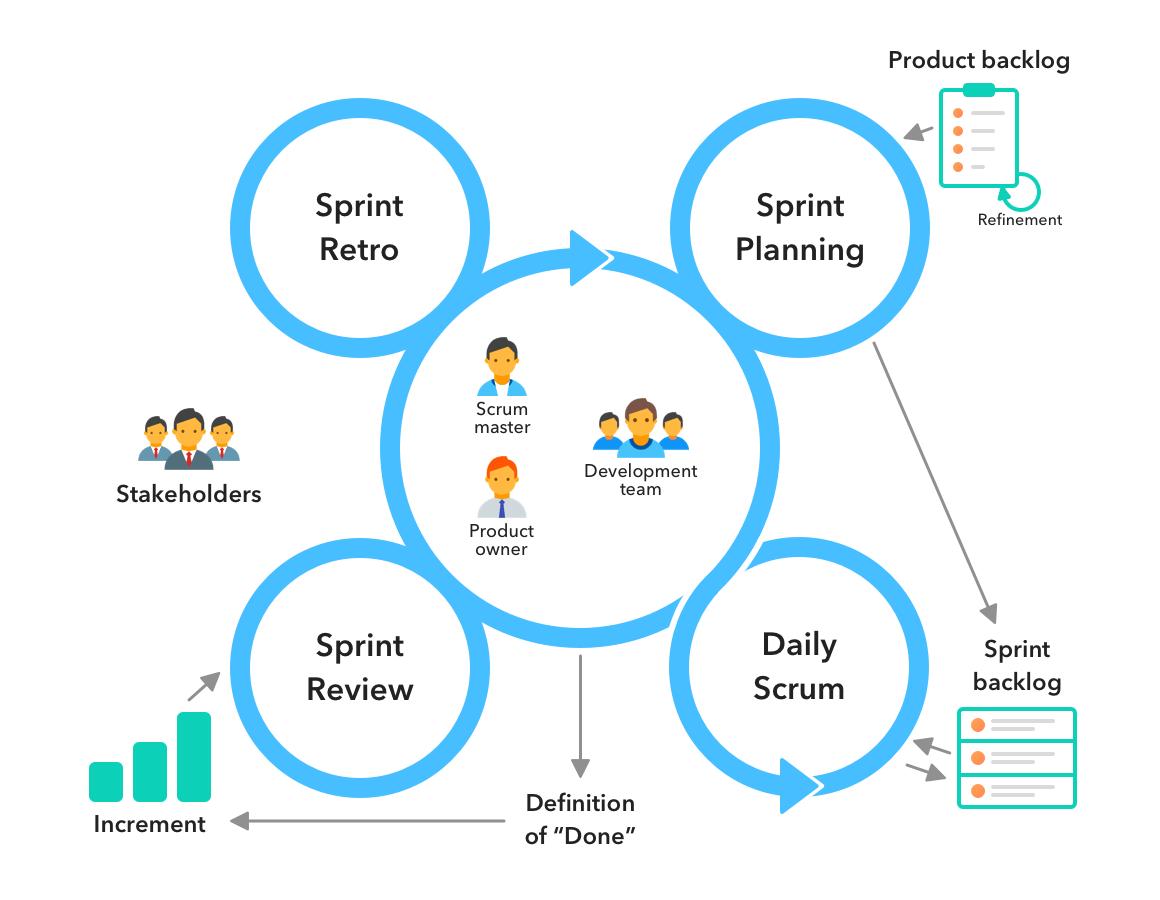
\includegraphics[width=0.75\linewidth]{Pictures/Scrum.jpeg}
	\caption{Framework Scrum \textbf{Source} \href{https://startinfinity.com/project-management-methodologies/scrum}{startinfinity.com})}
	\label{scrum}
\end{figure}


	\section{M\'ethodologies et frameworks choisis}
		Pour choisir la m\'ethodologie \`a adopter dans la r\'ealisation de notre projet, nous nous proposons d'en trouver une qui soit r\'ealisable dans notre environnement de travail. Consid\'erant ce dernier comme \'etant le param\`etre le plus contraignant dans notre cas. Ensuite nous d\'esirons qu'elle favorise la communication entre les diff\'erentes acteurs et qu'elle soit efficace.

		\paragraph{} Pour notre part, nous travaillons dans le contexte que d\'ecrivent les points suivants:
			\begin{itemize}
				\item[-] Nous habitons respectivement Mariani, Route Fr\`eres et Delmas.
				\item[-] Pour nous rencontrer en ville, deux d'entre nous doivent traverser des zones de non droit
				\item[-] La couverture r\'eseau \`a ces trois endroits n'est ni stable, ni similaire. Il peut donc arriver que l'un d'entre nous ne soit pas joignable via Whatsapp, Telegram ou appel t\'el\'ephonique \`a cause d'une panne de r\'eseau.
				\item[-] L'activit\'e des gangs arm\'es peut emp\^echer les d\'eplacement de n'importe lequel d'entre nous, \`a n'importe quel moment.
				\item[-] Au moment o\`u nous d\'emarrons le projet, nous ne disposons pas de toutes les connaissances n\'ecessaires pour sa r\'ealisation.
			\end{itemize}


		\paragraph{}Au d\'ebut, pour fonder les bases de notre collaboration avec le client, la m\'ethode utilis\'ee \'etait la m\'ethode Watherfall. Ensuite nous avons pris les d\'ecisions suivantes:
		\begin{enumerate}
			\item Pour des raisons de s\'ecurit\'e, nous devons limiter les rencontres en pr\'esentiel.

			\item Compte tenu de notre choix pour l'architecture du syst\`eme (voir chapitre~\ref{ChapArchitectureDuSysteme}), nous avons donc divis\'e le travail en cinq grandes parties autonomes, mais co-d\'ependantes:
				\begin{enumerate}
					\item R\'edaction du document de m\'emoire
					\item D\'eveloppement de l'interface utilisateur
					\item D\'eveloppement de l'application cot\'e serveur
					\item D\'eveloppement de la base de donn\'ees.
					\item D\'eploiement du site
				\end{enumerate}

			\item Chacun de nous est responsable de tout ce qui concerne le projet dans son ensemble maus se charge d'une ou d'au moins une partie en priorit\'e. Permettant \`a chacun de continuer \`a travailler m\^eme s'il se retrouve provisoirement isol\'e de l'\'equipe.
		\end{enumerate}






	 	\paragraph{} Compte tenu de nos objectifs, de notre contexte et environnement de travail et de nos contraintes nous utilisons la m\'ethode \textbf{Agile} \`a travers son Framework \textbf{Scrum} pour d\'eterminer des cycles de travail \`a court terme ensuite, suivant le contexte environnemental, nous utiliseront soit Scrum soit Waterfall pendant ces cycles.
	

		\newrefsection
			\chapter{Budget}

\begin{longtable}{ >{\centering\arraybackslash\bfseries}m{0.1\textwidth} >{\raggedright\arraybackslash}m{0.42\textwidth} >{\raggedright\arraybackslash}m{0.13\textwidth} >{\raggedright\arraybackslash}m{0.13\textwidth} >{\raggedright\arraybackslash}m{0.1\textwidth}}

        \hline
        \hline
        \rowcolor{TetTablo}
        \textbf{\large Service - Article} & \textbf{Description} & \textbf{Prix unitaire} & \textbf{Quantit\'e} & \textbf{Prix total}\\
        \hline
        \hline
        \endfirsthead

        \hline
        \hline
        \rowcolor{TetTablo}
        \textbf{\large Service - Article} & \textbf{Description} & \textbf{Prix unitaire} & \textbf{Quantit\'e} & \textbf{Prix total}\\
        \hline
        \hline
        \endhead

        \hline
        \endfoot

        \hline
        \hline
        \endlastfoot

        
		\rowcolor{mybrown}
		\multicolumn{5}{l}{\bfseries Mat\'eriel} \\
    \end{longtable}




	\part{Conception}
		\newrefsection
			\chapter{Mod\'elisation}


	En d\'eveloppement logiciel, la mod\'elisation est le fait d'associer une repr\'esentation abstraite et simplifi\'ee \`a un syst\`eme en vue de d\'ecrire sa structure, expliquer son fonctionnement, pr\'evoir des aspects de son comportement, et aussi de disposer d'un langage commun entre le client et l'\'equipe de d\'eveloppeurs.
	
	\section{UML}
		UML est un langage graphique qui permet de cr\'eer des mod\`eles qui serviront de support \`a la cr\'eation d'un syst\`eme. \\
		Le langage fournit 13 diagrammes repr\'esentant chacun une vue distincte du syst\`eme. Mod\'eliser un syst\`eme avec UML consiste \`a s\'electionner, parmi les 13 disponibles, ceux qui sont les plus adapt\'es au projet et qui, mis ensemble, le d\'ecrivent compl\`etement.\\
		
		
	\section{Diagramme de contexte}
		Le diagramme de contexte (Voir Figure~\ref{DiagrammeDeContexte}) montre relation entre un syst\`eme et les entit\'es externes qui interagissent avec lui. Notre syst\`eme interagit avec nos utilisateurs externes, \`a savoir le simple\_Utilisateur, l'administrateur et le SuperAdmin.
		
		\begin{figure}[!ht]
			\centering
			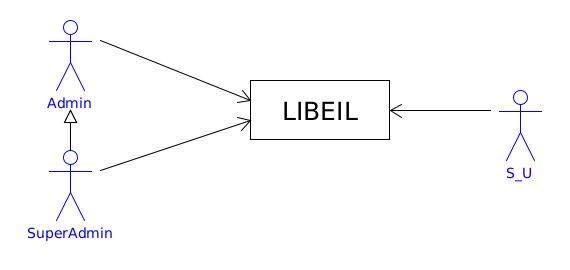
\includegraphics[width=0.5\linewidth]{Pictures/DiagrammeDeContexte.jpg}
			\caption{Le diagramme de contexte}
			\label{DiagrammeDeContexte}
		\end{figure}

	\section{Diagramme des cas d'utilisation}
		Les diagrammes de cas d'utilisation font ressortir les fonctionnalit\'es du syt\`eme que les utilisateurs vont exploiter pour interagir avec le syst\`eme.
		
		\paragraph{} Ci-apr\`es, nous pr\'esentons nos trois cas d'utilisations, \`a savoir le cas du simple\_utilisateur (Voir figure~\ref{CasUtilisationSU}), le cas de l'administrateurs (Voir figure~\ref{CasUtilisationAdmin}) et celui du SuperAdmin (Voir figure~\ref{CasUtilisationSuperAdmin}).
							
			
			
		\begin{figure}[!ht]
			\begin{minipage}{0.5\textwidth}
				\centering
				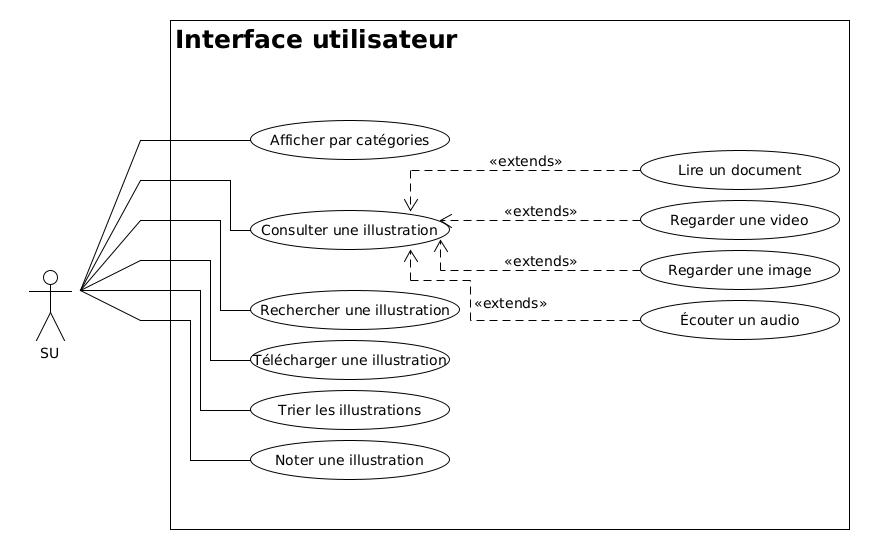
\includegraphics[width=0.9\linewidth]{Pictures/DiagrammeDesCasDUtilisationSU.jpg}
				\caption{Cas de Simple\_Utilisateur}
				\label{CasUtilisationSU}
			\end{minipage}
			\begin{minipage}{0.5\textwidth}
				\centering
				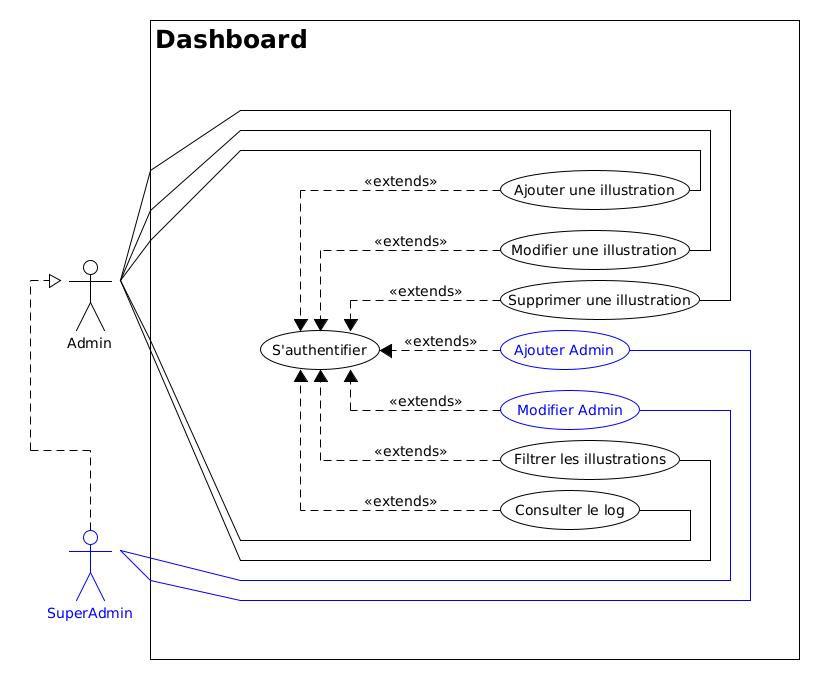
\includegraphics[width=0.9\linewidth]{Pictures/DiagrammeDesCasDUtilisationAdmin.jpg}
				\caption{Cas d'utilisation-Administrateurs}
				\label{CasUtilisationAdmin}
			\end{minipage}
		\end{figure}
			
			
	\section{Diagramme d'activit\'es}
		Le diagramme d'activit\'es (voir figure~\ref{DiagrammeDActivite}) repr\'esente le flux des activit\'es que les utilisateurs peuvent effectuer sur le syst\`eme. Il montre le flux de travail entre les utilisateurs et le syst\`eme \cite{DiagActivite}. Ce diagramme permet de mieux comprendre l'ordre dans lequel les op\'erations sont effectu\'ees et la fa\c{c}on dont elle sont coordonn\'ees. \\
			
			
			\begin{figure}[!ht]
				\centering
				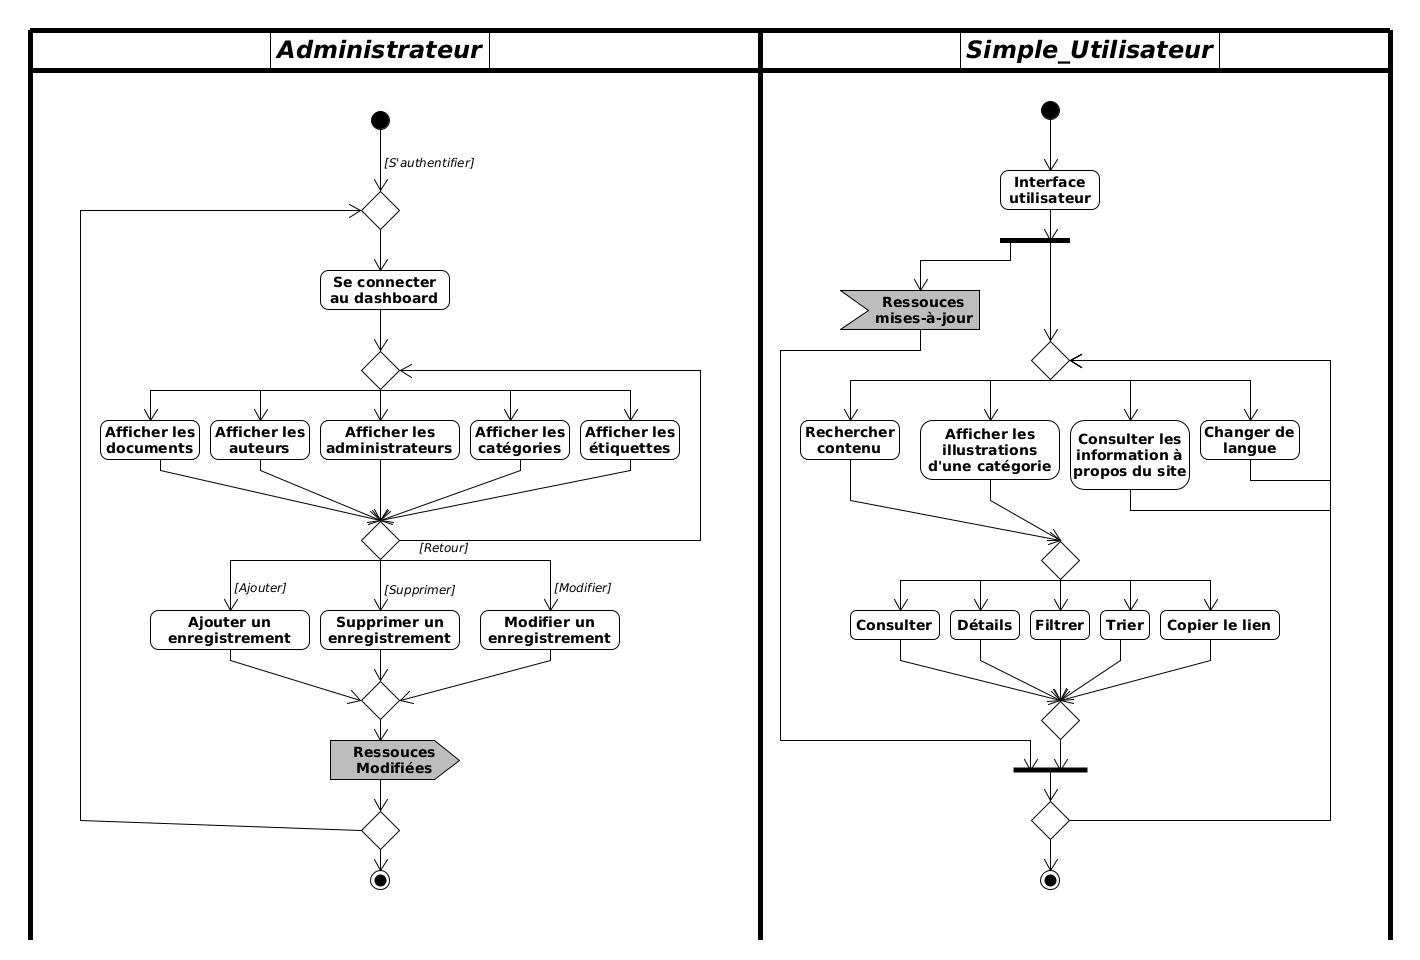
\includegraphics[width=0.75\linewidth]{Pictures/DiagrammeDActivites.jpg}
				\caption{Le diagramme d'activit\'es}
				\label{DiagrammeDActivite}
			\end{figure}
			
			
			

	\section{Diagramme de classes}

		
		Le diagramme de classe d\'ecrit la structure interne du syst\`eme en visualisant les diff\'erents types d'objets qui le constituent et les types de relations qui existent entre eux. Ce diagramme est fondamental pour la mod\'elisation du syst\`eme.
		
		\paragraph{} Dans notre cas, le diagramme des classes (voir Figure~\ref{DiagremmeClasses}) pr\'esente les 8  entit\'es du site, leur m\'ethodes ainsi que les relations entre elles.
	
		\begin{figure}[!ht]
			\centering
			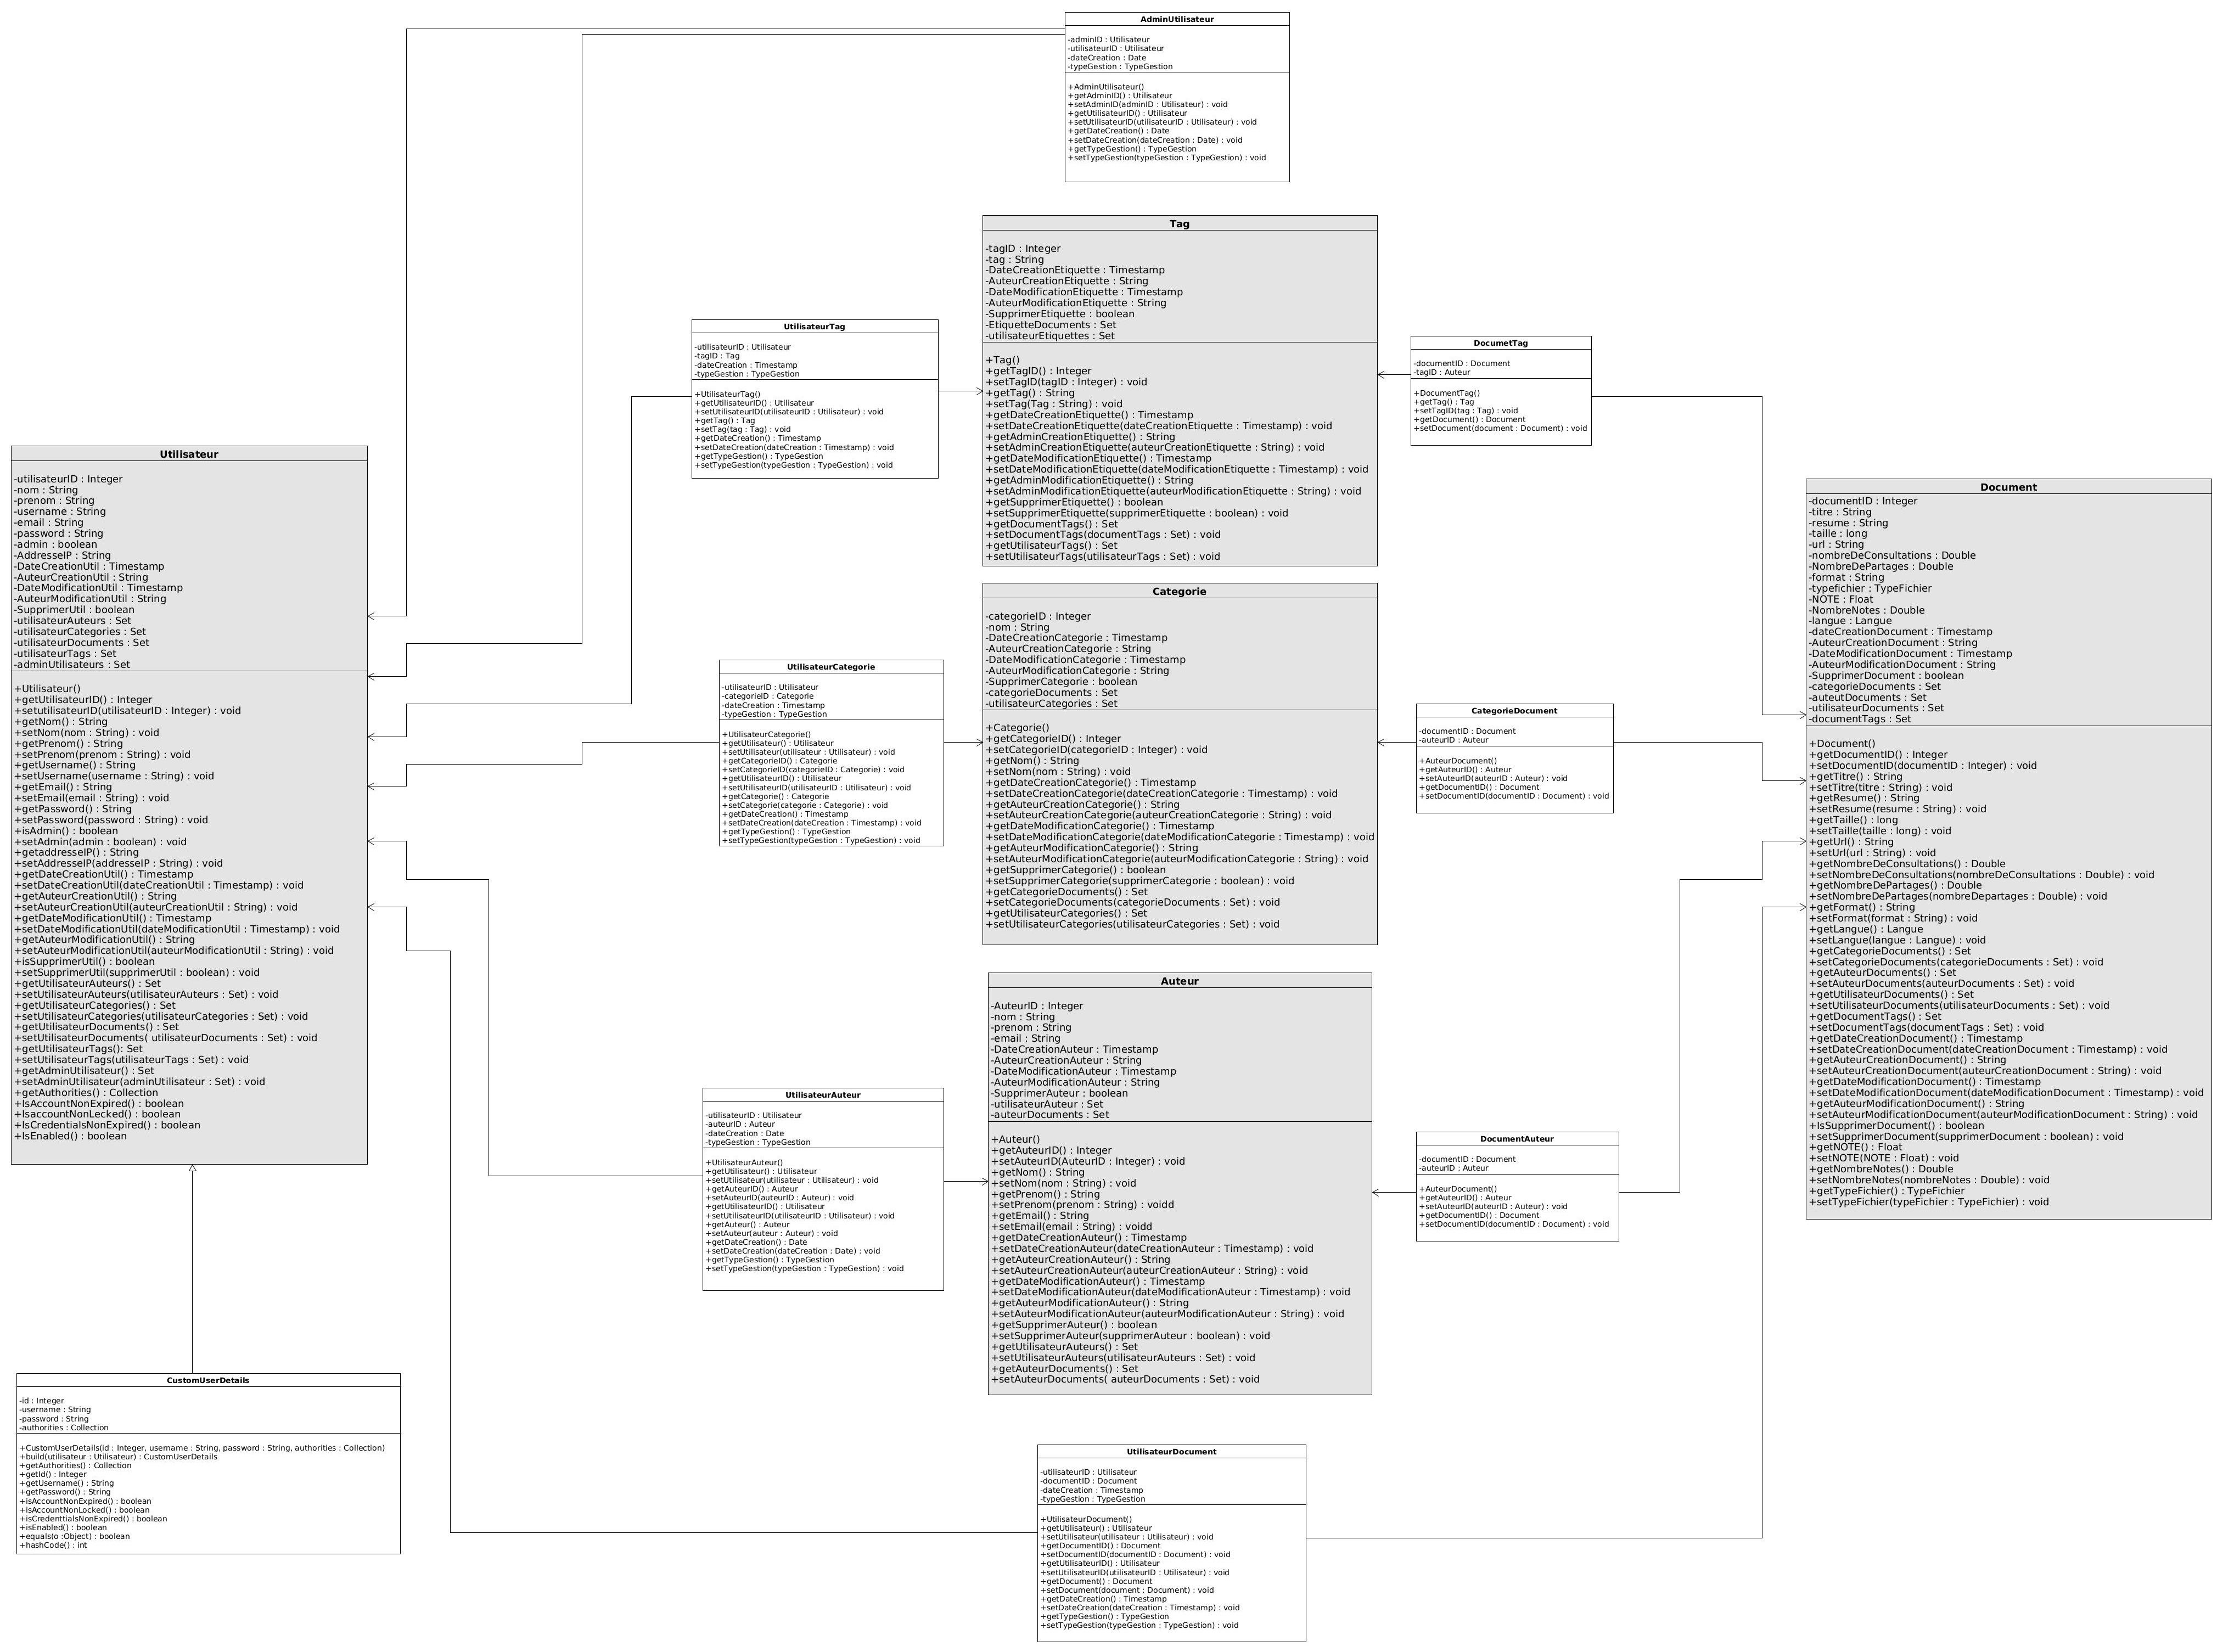
\includegraphics[width=0.7\linewidth]{Pictures/DiagrammeDeClasses.jpg}
			\caption{Le diagramme des classes}
			\label{DiagremmeClasses}
		\end{figure}



	\section{Diagrammes de s\'equence}
		Le diagramme de s\'equence repr\'esente les principaux objets qui constituent le logiciel et la suite de requ\^etes et messages entre les objets au cours des op\'erations CRUD \`a travers celui-ci. Il montre comment divers composants d'un syst\`eme interagissent les uns avec les autres pour accomplir chacune des t\^aches \cite{DiagrammeSequence}. 
		
		\subsection{Cas du simple\_utilisateur}
			\begin{figure}[!ht]
				\centering
				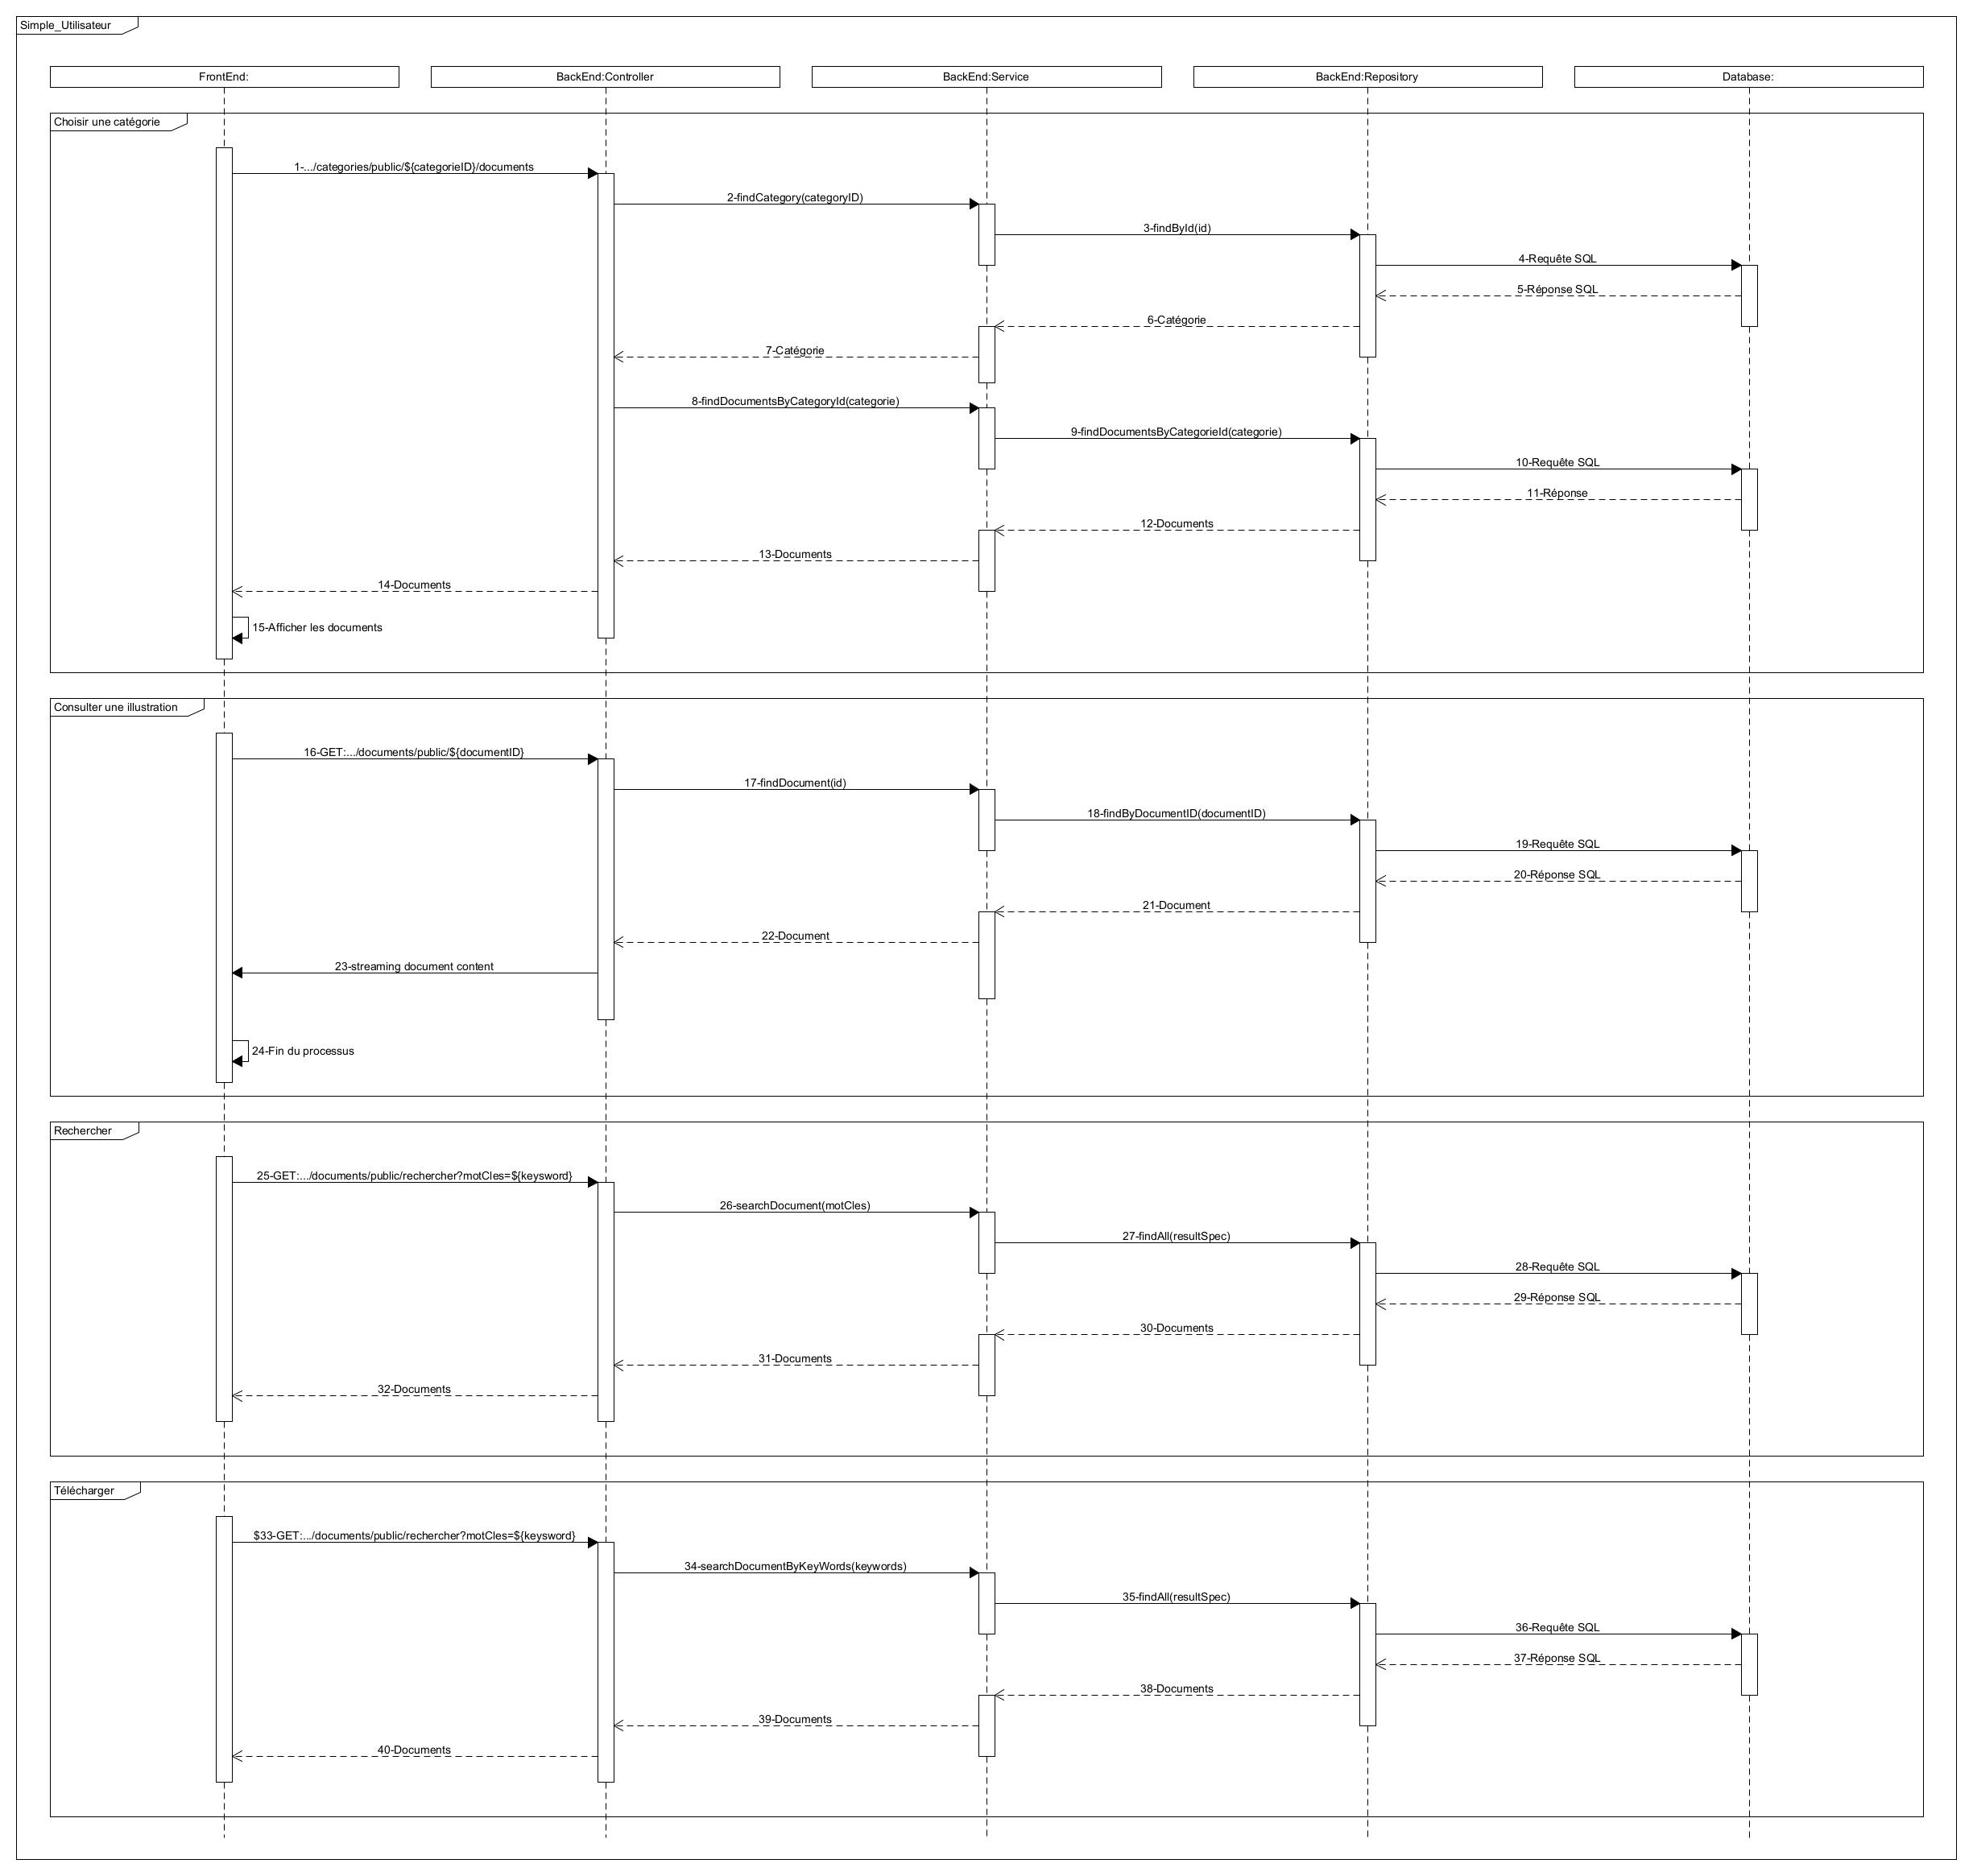
\includegraphics[height=0.7\textheight]{Pictures/DiagrammeDeSequenceSimpleUtilisateur.jpg}
				\caption{Le diagramme de s\'equences - Cas du simple\_utilisateur}
				\label{DiagrammeDeSequenceSU}
			\end{figure}

		\newpage
		\subsection{Cas de l'administrateur}
			\begin{figure}[ht]
				\centering
				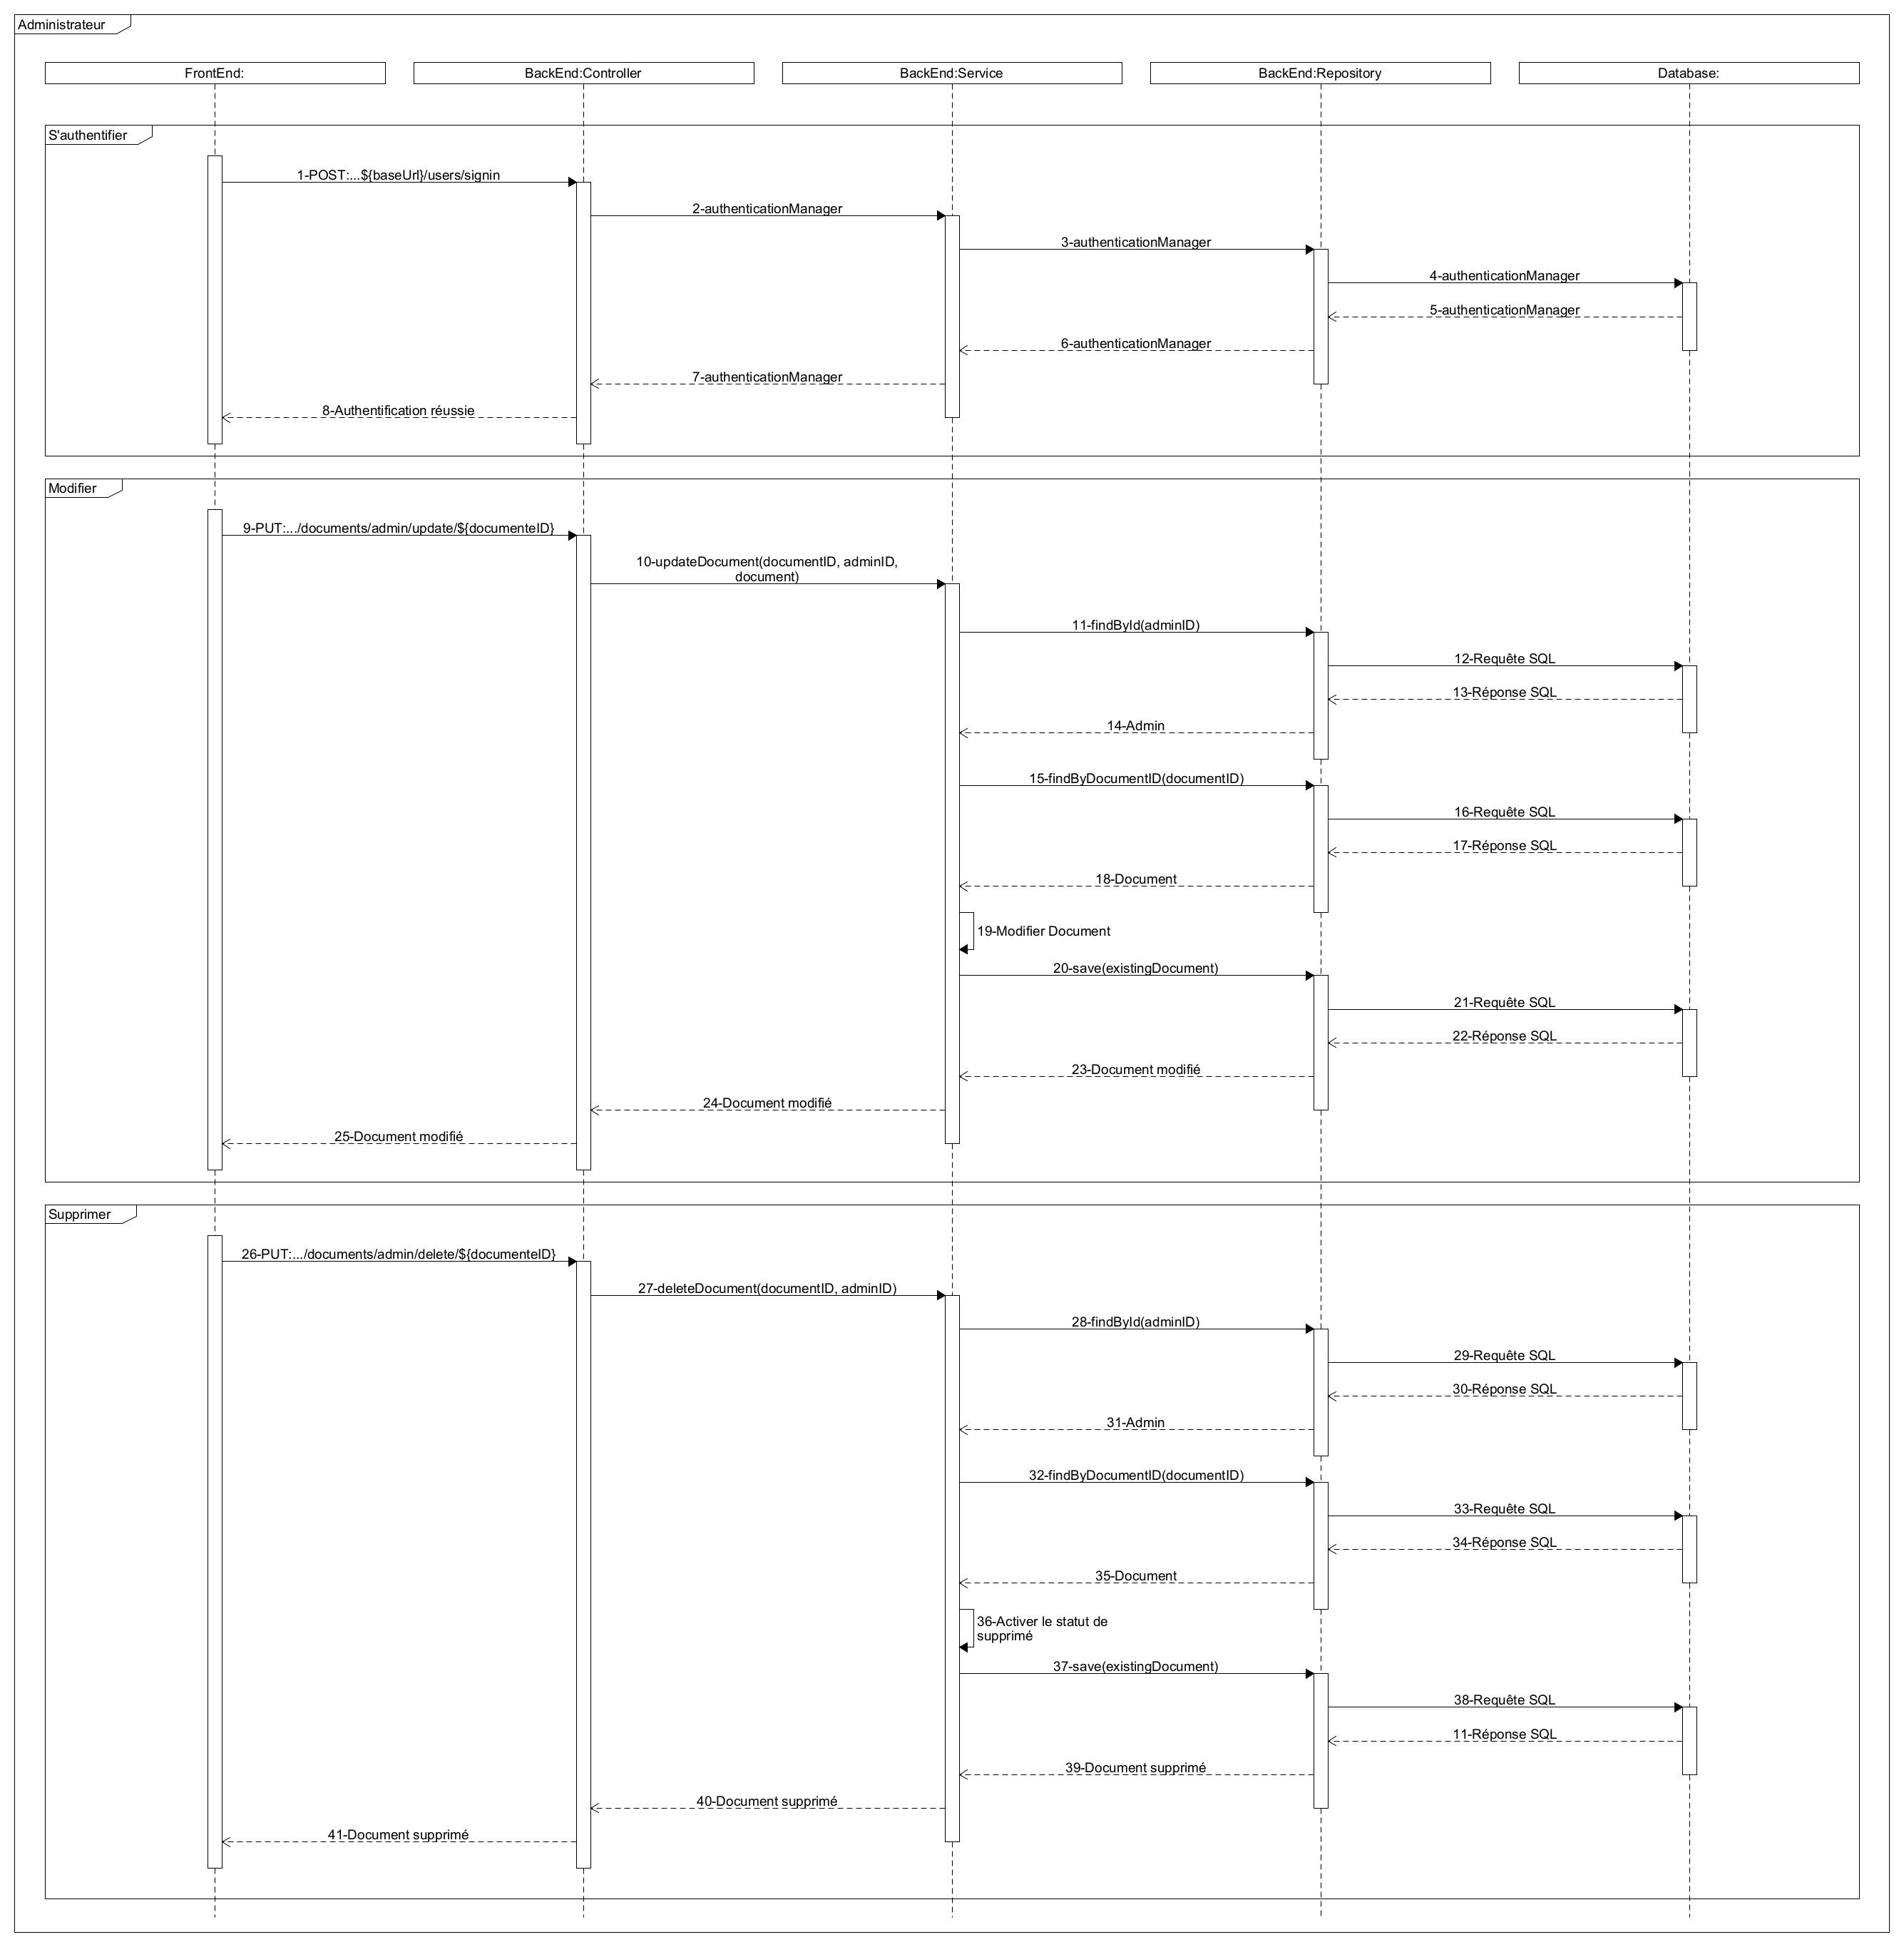
\includegraphics[height=0.7\textheight]{Pictures/DiagrammeDeSequenceAdministrateur.jpg}
				\caption{Le diagramme de s\'equences - Cas de l'administrateur-Partie 1}
				\label{DiagrammeDeSequenceAdmin1}
			\end{figure}
			
			\begin{figure}[ht]
			\centering
			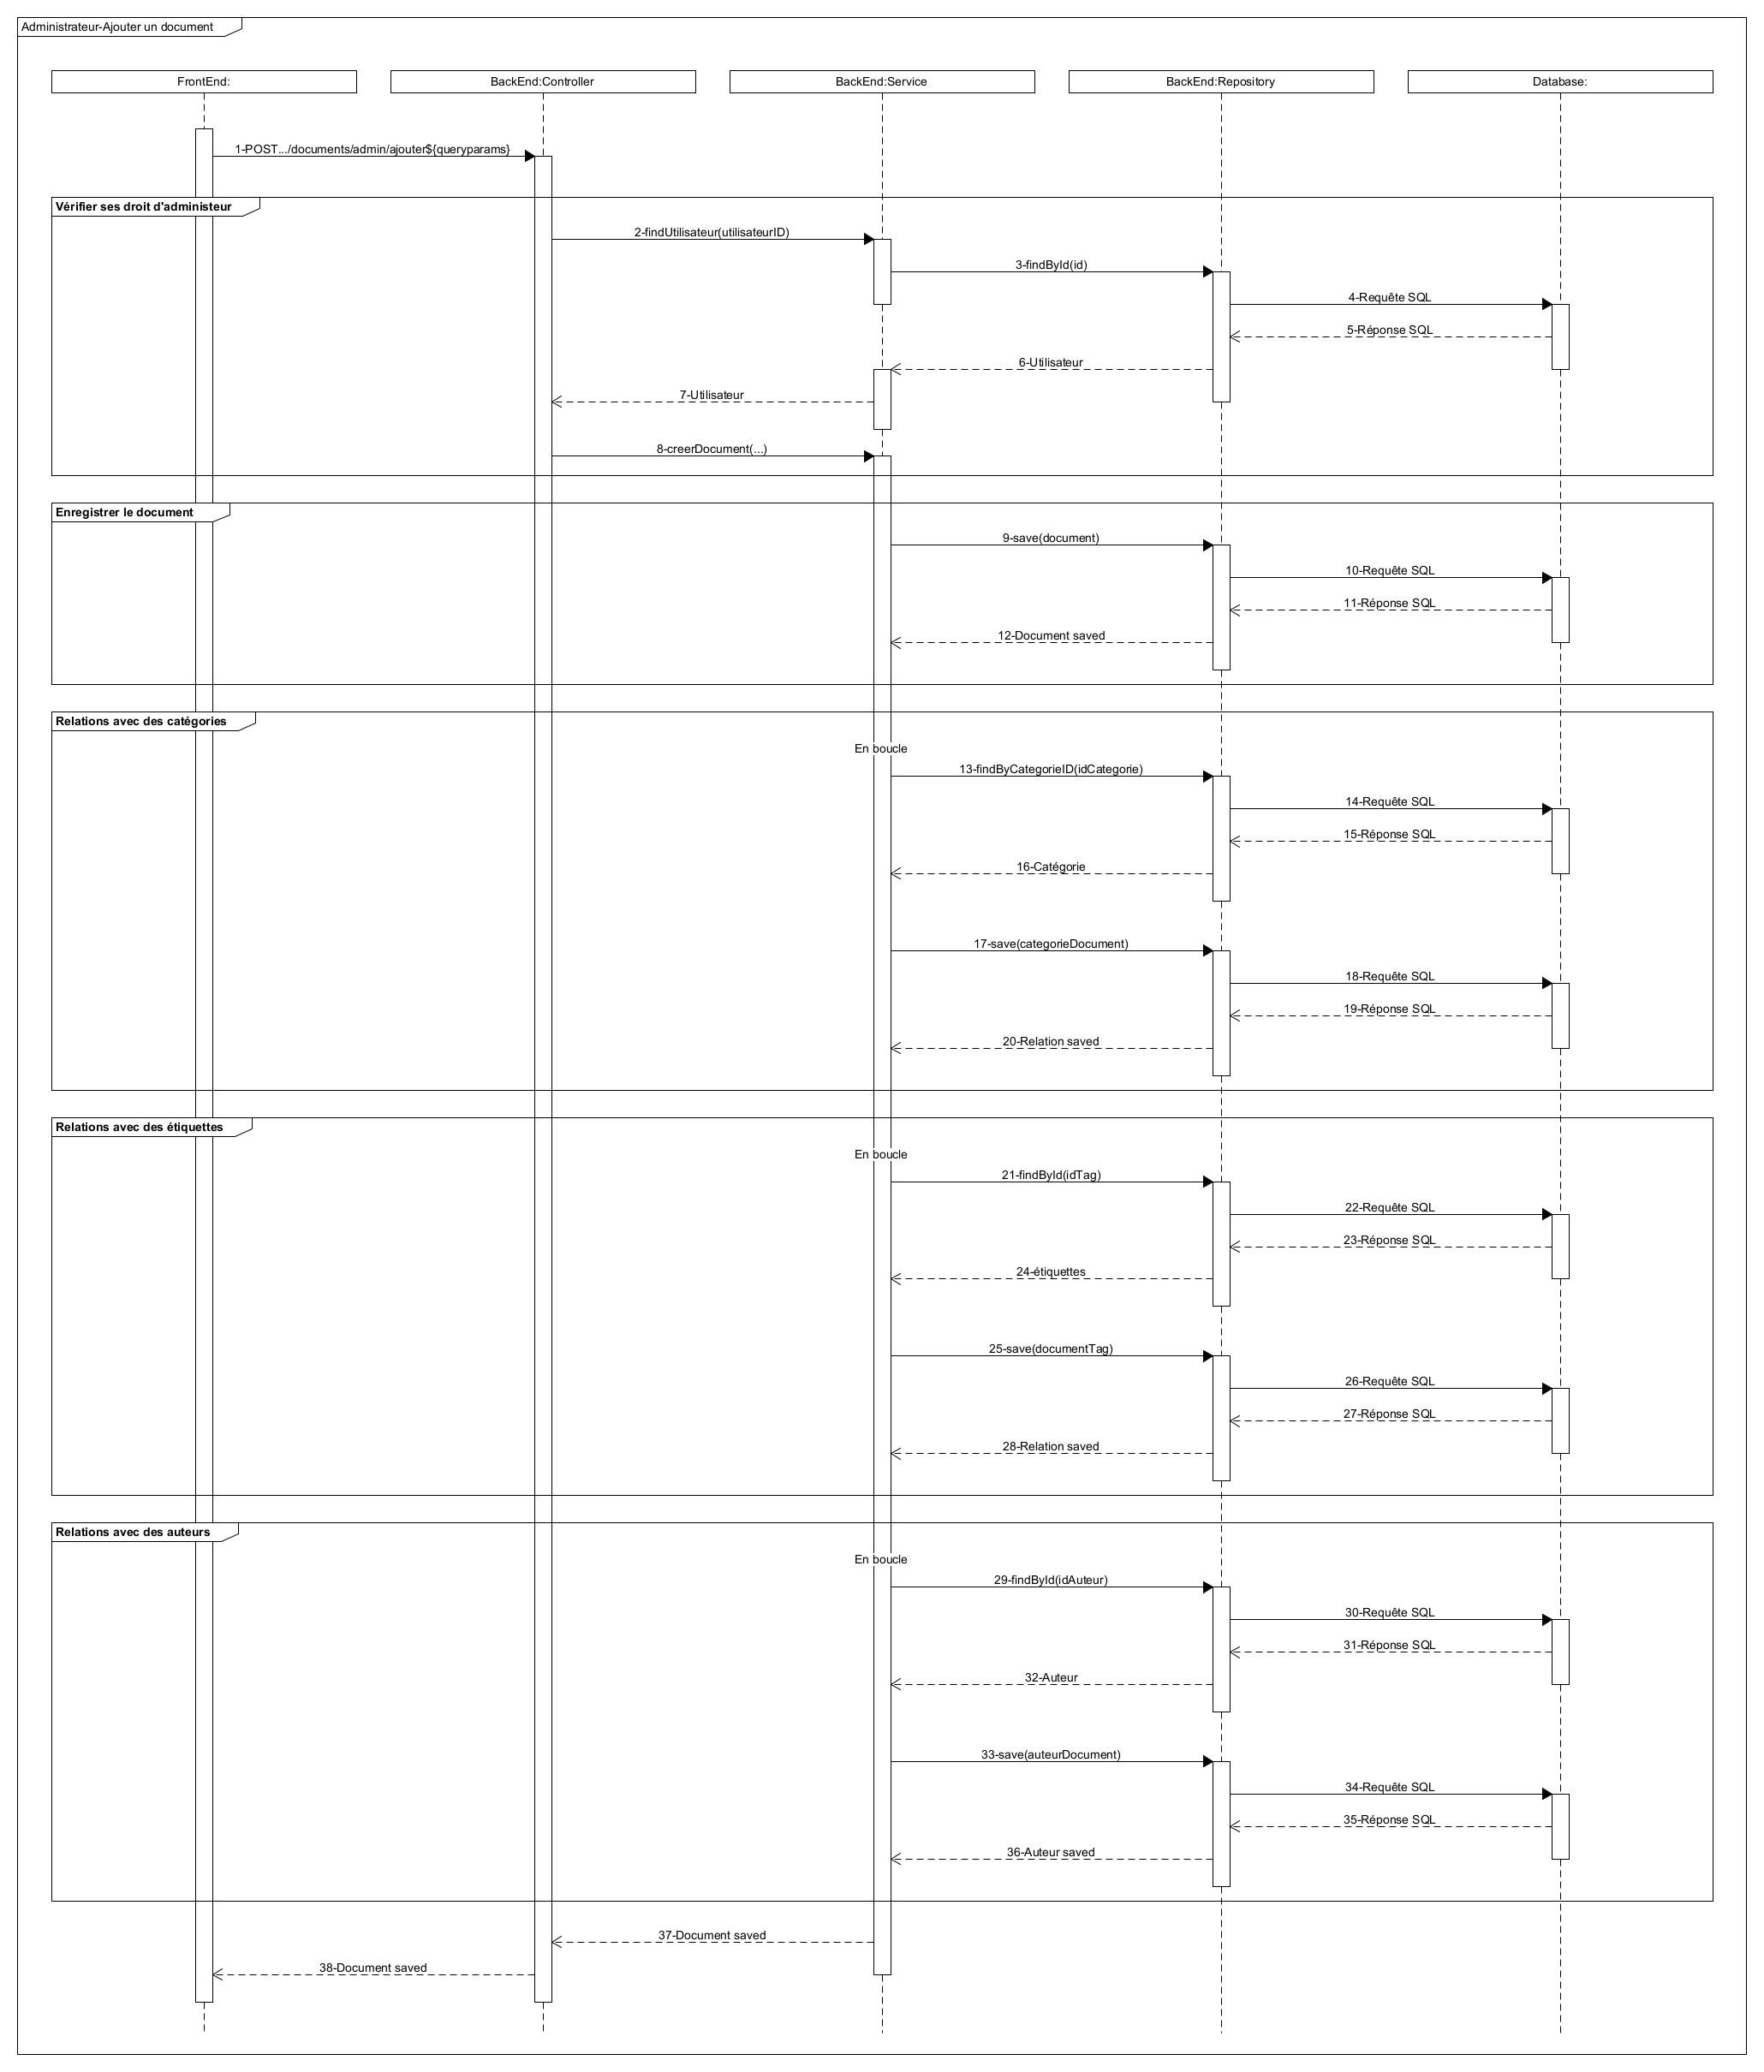
\includegraphics[height=0.7\textheight]{Pictures/DiagrammeDeSequenceAJouterDocument.jpg}
			\caption{Le diagramme de s\'equences - Cas de l'administrateur-Partie 2}
			\label{DiagrammeDeSequenceAdmin2}
			\end{figure}





		\newrefsection
			\chapter{Structure du site}
\section{MPAs \textit{versus} SPAs \cite{ArchitectureWebApp}}
Traditionnellement, les sites webs \'etaient constitu\'es d'un ensemble de pages diff\'erentes stock\'es sur le serveur et qui seront transmis aux visiteurs suivant au demande. Cette fa\c{c}on de faire est toujours utilis\'e aujourdh'ui puisqu'il a ses avantages. Toutefois, il existe aussi la possibilit\'e de cr\'eer des sites Webs avec une seule page. 


\subsection{Pages Web traditionnels - MPAs (Multi-Page Applications)}
Les applications Web multi-pages impliquent peu de comportement c\^ot\'e client, mais s'appuient plut\^ot sur le serveur pour toutes les navigations, requ\^etes et mises \`a jour que l'application pouvait avoir besoin d'effectuer. Chaque nouvelle op\'eration effectu\'ee par l'utilisateur serait traduite en une nouvelle requ\^ete web, avec pour r\'esultat un rechargement complet de la page dans le navigateur de l'utilisateur. \\

Amazon et Google Docs sont des exemples de telles pages.

\subsection{Applications Web \`a page Unique - SPAs (Single-Page Applications)}
Une application \texttt{Web} \`a page unique (SPA) fonctionne dans un navigateur Web et ne charge qu'une seule page. Il n'a pas besoin de recharger la page pendant son utilisation, surtout que la plupart de son contenu reste le m\^eme, par cons\'equent, seule une partie doit \^etre mise \`a jour. Lorsque le contenu doit \^etre mis \`a jour, le SPA le fait via des APIs.\\
De cette façon, les utilisateurs peuvent consulter un site Web sans charger l'int\'egralit\'e de la nouvelle page ni les donn\'ees du serveur. En cons\'equence, les performances augmentent et vous avez l'impression d'utiliser une application native. Il offre une exp\'erience Web plus dynamique aux utilisateurs. \\

Gmail, Facebook, Trello et Google Maps sont tous des applications \`a page unique qui offrent une exp\'erience utilisateur exceptionnelle dans le navigateur sans rechargement de page.


\subsection{Diff\'erences}
Les SPAS ont un temps de chargement plus longue, mais offrent des performances plus rapides et une navigation fluide apr\`es le chargement. Les MPAs peuvent \^etre relativement lents et n\'ecessitent une connexion Internet de premier ordre, notamment en ce qui concerne les \'el\'ements graphiques.\\

Les MPAs sont efficaces lorsque :
\begin{itemize}
	\item[-] Les exigences c\^ot\'e client de l'application sont simples, voire en lecture seule.
	\item[-] L'application fonctionne dans les navigateurs sans prise en charge de JavaScript.
	\item[-] L'application est destin\'ee au public et b\'en\'eficie de la d\'ecouverte et des r\'ef\'erences des moteurs de recherche.
\end{itemize}

Les SPAs sont efficaces lorsque :
\begin{itemize}
	\item[-] L'application pr\'esente une interface utilisateur riche avec de nombreuses fonctionnalit\'es.
	\item[-] L'\'equipe est familiaris\'ee avec le d\'eveloppement JavaScript, TypeScript ou Blazor WebAssembly.
	\item[-] L'application expose une API pour d'autres clients (internes ou publics).
\end{itemize}

\vspace{1cm}

\begin{table}[!ht]
	\centering
	\begin{tabular}{ | a || m{0.2\textwidth}  m{0.2\textwidth}|}
		%					\hline
		\rowcolor{lightgray}
		{\Large \textsc{Facteurs}} & \textbf{MPA} & \textbf{SPA}\\
		\hline
		\hline
		\textbf{Familiarit\'e de l'\'equipe avec JavaScript ou TypeScript} & Minimale & Requise\\
		\hline
		\textbf{Gestion du navigateur sans script} & Prise en charge & Non prise en charge \\
		\hline
		\textbf{Comportement minimal des applications c\^ot\'e client} &	Bien adapt\'e & Bien adapt\'e \\
		\hline
		\textbf{Interface utilisateur riche et complexe} &	Limit\'e & Bien adapt\'e \\
		\hline
		\textbf{D\'eveloppement} & Simple & Complexe\\
		\hline
		\textbf{Visibilit\'e sur les moteurs de recherche} & \'Elev\'ee & Faible \\
		\hline
		\textbf{Changement par un non-d\'eveloppeur} & Prise en charge & Non prise en charge\\
		\hline
	\end{tabular}
	\caption{Tableau r\'ecapitulatif - Principales crit\`eres de choix entre MPAs et SPAs}
	\label{tableChoixEntreMPAetSPA}
\end{table}

\paragraph{} Pour garantir un excellent service aux utilisateurs du logiciel, g\'erer les divers fonctionnalit\'es requises pour notre syst\`eme sans erreur, nous avons opt\'e pour le mod\`ele SPA (Single Page Application). Nous devrons donc trouver un moyen pour augmenter la visiblit\'e du site sur les moteurs de recherche et  d\'evelopper un outils de gestion du logiciel pour r\'epondre aux exigences du projet (Voir Sections~\ref{SectQualiteDuSysteme} et~\ref{SectionBesoinsFonctionnels}).



\subsubsection{Fonctionnement du mod\`ele SPA}

\begin{figure}[!ht]
	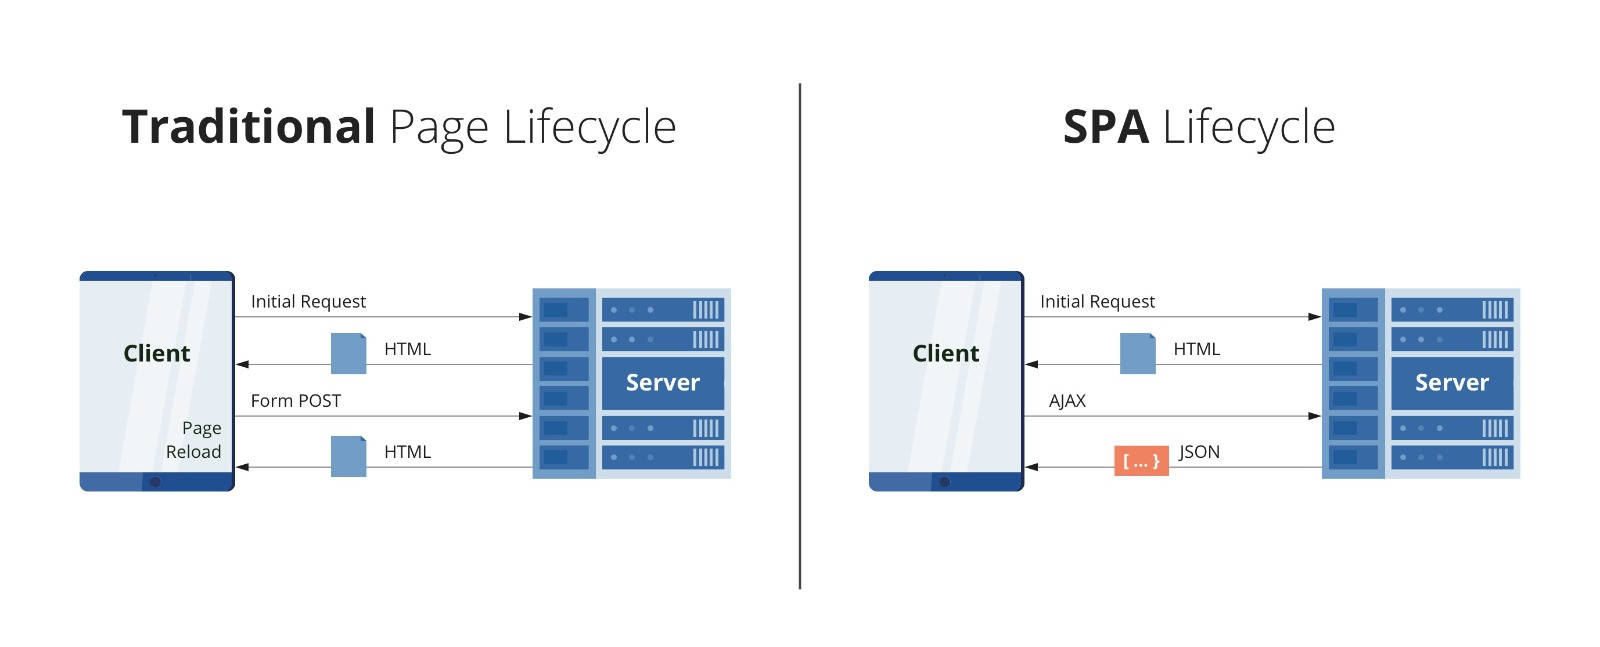
\includegraphics[width=0.7\linewidth]{Pictures/SPALifeCycle.jpg}
	\centering
	\caption{Cycle de vie d'un SPA par rapport \`a celui d'un MPA\cite{CycleDeVieMPAvsSPA}}
	\label{FigSPA}
\end{figure}


Le mod\`ele SPA repose sur les principes suivants :
\begin{enumerate}
	\item Le SPA utilise principalement des technologies de rendu c\^ot\'e client, comme JavaScript, TypeScript et autres pour g\'erer la logique de l'interface utilisateur et communiquer avec le serveur via des API web.
	\item Le SPA charge initialement le code HTML, CSS et JavaScript n\'ecessaire pour afficher la page web. Ensuite, il ne charge que les donn\'ees n\'ecessaires pour mettre \`a jour le contenu de la page, en utilisant des formats l\'egers comme JSON ou XML.
	\item Le SPA utilise le concept de routage c\^ot\'e client, qui consiste \`a modifier l'URL de la page sans recharger la page, en utilisant \texttt{l'API History} du navigateur. Ainsi, le SPA peut offrir une navigation fluide et intuitive, tout en conservant la possibilit\'e d'utiliser les boutons Pr\'ec\'edent et suivant du navigateur.
	\item Le SPA offre une exp\'erience utilisateur plus rapide, plus r\'eactive et plus proche d'une application native, car il \'evite les temps de chargement et les rafraîchissements de la page. Il peut \'egalement fonctionner hors ligne, en utilisant des technologies comme le \texttt{Service Worker} ou le \texttt{Local Storage}.
\end{enumerate}


\section{Architecture du syst\`eme\cite{Architecture3Niveau}}
\label{ChapArchitectureDuSysteme}
L'architecture d'un syst\`eme est la mani\`ere de concevoir et d'organiser les diff\'erents \'el\'ements qui le composent. Il s'agit d'une repr\'esentation abstraite d'un syst\`eme exprim\'ee essentiellement \`a l'aide des composants du logiciels et de leurs interactions. L'architecture d'un syst\`eme permet de d\'efinir la structure, le comportement, la qualit\'e et les contraintes du syst\`eme, en fonction des besoins et des objectifs du projet. Elle facilite par cons\'equent la conception, le d\'eveloppement, le d\'eploiement et la maintenance de celui ci. Il existe plusieurs architecture possible pour une application web dont: l'architecture monolithique, les architectures \`a  N-niveaux, Architecture hexagonal (Aussi appel\'e Architecture Port-et-adapter)  \\

\subsection{Architecture de \projectName}
L'architecture adopt\'ee pour notre syst\`eme est l'architecture \`a trois niveaux (appel\'ee architecture \texttt{3-tiers}) client/application/ressource (Voir Figures~\ref{FigArchitecture} et~\ref{FigArchitecture1}).  Le principal avantage de l'architecture \`a trois niveaux r\'eside dans la s\'eparation logique et physique des fonctionnalit\'es. Chaque niveau peut fonctionner sur un syst\`eme d'exploitation et une plate-forme de serveur distincts (par exemple : un serveur Web, un serveur d'applications, un serveur de base de donn\'ees).\\
Outre cet avantage essentiel, elle offre une plus grande flexibilit\'e du fait qu'un \'el\'ement peut \^etre remplac\'e sans devoir changer toute l'architecture, une s\'ecurit\'e peut \^etre impl\'ement\'ee \'e chaque service et \`a chaque niveau. Et enfin, puisque les t\^aches sont partag\'ees elle offre de meilleures performances surtout une fiabilit\'e am\'elior\'ee. Elle est aussi r\'esistante aux pannes puisqu'une panne dans un niveau est moins susceptible d'avoir un impact sur la disponibilit\'e ou les performances des autres niveaux.

	\begin{figure}[ht]
		\centering
		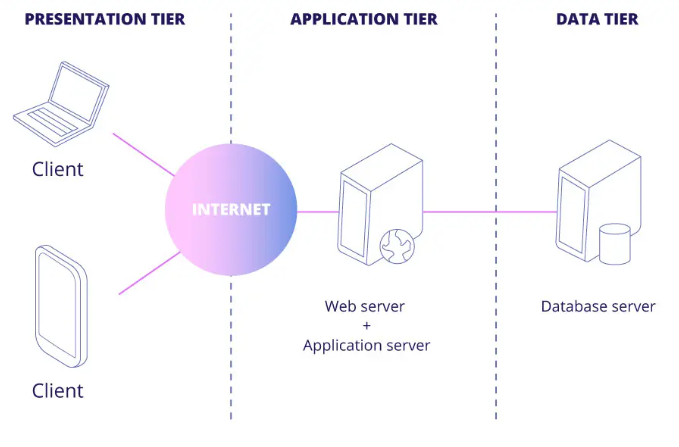
\includegraphics[width=0.5\textwidth]{Pictures/SystemStruct.png}
		\caption{Architecture physique \`a trois niveaux\cite{SourceFigArchitecture}}
		\label{FigArchitecture}
	\end{figure} 


L'architecture \`a trois niveaux organise les applications en trois niveaux informatiques logiques et physiques : le niveau de pr\'esentation, ou interface utilisateur ; le niveau application, o\`u les donn\'ees sont trait\'ees ; et le niveau des donn\'ees, o\`u  les donn\'ees associ\'ees \`a l'application sont stock\'ees et g\'er\'ees.
\subsubsection{Partie cliente - Front-End}
Cette partie est constitu\'ee des nœuds et elle consiste aussi \`a la r\'ealisation des diff\'erentes interfaces de l'application et leur affichage. En gros ce sont les demandeurs de ressources.

\subsubsection{Partie serveur (serveur d'application)}
Permet de r\'epondre de mani\`ere automatique \`a des demandes envoy\'ees par la partie cliente. C'est elle qui se charge de fournir la ressource tout en faisant appel \` un autre serveur (serveur base de donn\'ees).

\subsubsection{Partie serveur base de donn\'ees}
Permet l'insertion, la consultation des donn\'ees et la mise \`a jour du syst\`eme. Elle fournit un service au serveur d'application.



		\newrefsection
			\chapter{Outils de construction}
\label{ChapOutilsDev}


\begin{table}[!ht]
	\centering
	\begin{tabular}{| m{6cm} | m{5cm} |}
		\hline
		\multirow{4}{6em}{\textbf{\large{\textcolor{myblue}{Document}}}} & \TeX Live 2022 \\
		& Jabref 3.8.2\\
		&\TeX Studio 4.8.1\\
		& UMLet 15.1\\ 
		\hline
		\textbf{\large{\textcolor{myblue}{Application serveur}}} & Spring Boot 2.7.14\\
		\hline
		\multirow{2}{6em}{\textbf{\large{\textcolor{myblue}{Base de donn\'ees}}}} & Mariadb Server 10.6.16\\
		& Dbeaver 23.3.4\\
		\hline
		\textbf{\large{\textcolor{myblue}{Interface utilisateur}}} & Angular 17.3.5\\
		\hline 
		\multirow{2}{6em}{\textbf{\large{\textcolor{myblue}{D\'eploiement}}}} & Docker 26.1.3 \\
		& Nginx 1.25.5-alpine\\
		\hline 
	\end{tabular}
	\label{TabRecapOutils}
	\caption{Tableau r\'ecapitulatif - Outils utilis\'es}
\end{table}


\paragraph{}Pour concevoir, d\'evelopper, d\'eployer et maintenir un syst\`eme, il est essentiel de choisir et d'utiliser de bons outils technologiques. \\
Dans notre cas, un outil est bon s'il est:
	\begin{itemize} 
		\item[-] \textbf{Efficace}\\ 
		C'est-\`a-dire qu'il effectue r\'eellement le travail pour lequel il est choisi
		\item[-] \textbf{Gratuit}\\
		Sauf dans un cas exceptionnel et/ou \`a la d\'ecision du client, conform\'ement aux exigences qui nos ont \'et\'e faits, nous n'utiliserons que des outils gratuits.
		\item[-] \textbf{Dans notre champ de comp\'etence}\\
		Ce travail \'etant r\'ealis\'e dans un cadre acad\'emique en tant que notre travail de fin d'\'etude, nous utiliserons de pr\'ef\'erence les connaissances et comp\'etence que nous avons acqu\'eri pendant l'\'etude en question. De ce fait, nous choisirons de pr\'ef\'erences outils que nous ma\^itrisons d\'ej\`a, ou dont nous disposons des pr\'erequis pour les  ma\^itriser. 
	\end{itemize}

	\paragraph{}Ainsi, nous allons \'evaluer les diff\'erentes options disponibles sur le march\'e en tenant, aussi, compte des objectifs, besoins et contraintes du projet suivant les diff\'erents crit\`eres : Performance, s\'ecurit\'e, fiabilit\'e, compatibilit\'e, \'evolutivit\'e, co\^ut, etc. pour pouvoir s\'electionner les outils que nous utiliserons. Pour chaque outils choisi, nous prendrons sa derni\`ere version \`a garantir un support sur le long terme. Ce chapitre pr\'esente nos diff\'erents choix technologiques en ce qui concerne le d\'eploiement du site, la cr\'eation du \texttt{document de m\'emoire}, de l'\texttt{Application serveur}, de l'\texttt{Interface utilisateur} ainsi que la \texttt{Base de donn\'ees}.
	
	\section{Documentation}
	
		\subsection{\LaTeX 
\includegraphics[height=2ex]{Pictures/latexLogo.png}}
			Conform\'ement aux exigences de notre client, nous utilisons \LaTeX\ comme technologie pour r\'ediger ce document.\\
			
			\LaTeX\ est un syst\`eme de cr\'eation de documents qui favorise une composition de haute qualit\'e. Il encourage les auteurs \`a ne pas trop se soucier de l'apparence de leurs documents mais \`a se concentrer sur l'obtention du bon contenu\cite{LatexOfficiel}.\\
			La technologie consiste en un langage de programmation qui utilise des balises\footnote{Instructions cod\'ees servant \`a caract\'eriser certains \'el\'ements d'un document\cite{BalisesLeRobert}} pour d\'efinir la structure et la mise en forme de documents et d'une distribution \TeX\footnote{Comme Mac\TeX ,\TeX Live ou Mac\TeX} qui est un logiciel qui interpr\`ete les codes source pour produire le document programm\'e. Le terme \LaTeX\ peut \^etre utilis\'e pour faire r\'ef\'erence, soit au langage, soit au moteur \TeX , soit \`a la technologie dans un sens g\'en\'eral.
	
			\paragraph{}Nous utilisons la distribution \TeX Live avec pdflatex comme compilateur. Elle fournit tous les services dont nous avons besoin, et est tr\`es bien document\'e en ligne ce qui facilite sa prise en main.
				
				
		\subsection{\TeX Studio 
\includegraphics[height=2ex]{Pictures/texstudioLogo.png}}
			\TeX Studio est un environnement de cr\'eation de documents pour \LaTeX . Le programme est libre et opensource. Il fournit une interface riche et claire facilitant la cr\'eation.\cite{TexStudio}
				
		\subsection{JabRef 
\includegraphics[height=2ex]{Pictures/jabrefLogo.png}}
			JabRef est un logiciel gratuit et open source qui aide \`a collecter, organiser, modifier, stocker et citer la litt\'erature et les recherches scientifiques dans un document. Il prend en charge divers formats de r\'ef\'erence, l'importation de texte int\'egral, les catalogues en ligne, les styles de citation et bien plus encore.\cite{jabref}\\
			Nous utilisons aussi JabRef pour cr\'eer un fichier de bibliographie.
	
		\subsection{UMLet 
\includegraphics[height=2ex]{Pictures/umletLogo.png}}
			UMLet est un outil UML gratuit et open source dot\'e d'une interface utilisateur simple qui permet de dessiner rapidement des diagrammes UML \`a partir de texte brut, de les partager via des exportations vers eps, pdf, jpg, svg et presse-papiers, et de d\'evelopper de nouveaux diagrammes personnalis\'es. \cite{umlet}\\
			Nous l'utilisons pour construire les diff\'erents diagrammes UML.
			
			
			\begin{table}[ht]
				\centering
				\begin{tabular}[pos]{ | b | m{0.25\textwidth} m{0.25\textwidth} |}
					\rowcolor{lightgray}
					
					& \textbf{\textsc{\large{Type}}} & \textbf{\textsc{\large{Commentaires}}}\\
					\hline
					\textbf{\LaTeX} & Langage de balisage & Permet la composition(Typesetting) d'un document\\
					\textbf{\TeX Live} & Distribution de \LaTeX & Permet de compiler les codes sources en \LaTeX \\
					\textbf{\TeX Studio} & Environnement de d\'eveloppement en \LaTeX & Facilite la cr\'eation en \LaTeX \\
					\hline
					\textbf{UMLet} & Outil de mod\'elisation & Permet le design des diagrammes de mod\'elisation \\
					\hline
					\textbf{JabRef} & Outil de gestion bibliographique & Aide \`a la cr\'eation d'un fichier .bib qui servira de source pour les r\'ef\'erences bibliographiques du document \\
					\hline
				\end{tabular}
				\caption{Tableau r\'esumant les outils et technologies utilis\'es dans la c\'eation du document}
				\label{TabOutilDoc}
			\end{table}

	\section{Application serveur}
		L'application serveur g\`ere la logique et les services de l'application. Il s'agit de l'ensemble des modules, et des API traite les requ\^etes provenant de l'interface utilisateur et communique avec la base de donn\'ees. Pour le cr\'eer, nous utilisons les outils suivants:
			
		\subsection{Java 
\includegraphics[height=3ex]{Pictures/javaLogo.jpeg}}
			Java est un langage de programmation orient\'e objet de haut niveau, bas\'e sur des classes. Il est fr\'equemment utilis\'e pour cr\'eer des solutions back-end complexes. Java est \`a la fois simple et s\^ur. Ce langage de programmation permet de cr\'eer des applications \'evolutives et faciles \`a maintenir gr\^ace \`a une grande compatibilit\'e et \`a une vari\'et\'e d'outils et de biblioth\`eques entres autres autres avantages.\\
			Parmi les caract\'eristiques qui nous ont pouss\'es \`a choisir ce langage, nous citons les suivants :
			\begin{itemize}
				\item[-] \textbf{Simple et \'evolutif}\\
					Avec l'\'edition entreprise, le serveur peut ex\'ecuter plusieurs instances Java pour une mise \`a l'\'echelle automatique.  De plus, tous les composants Java dont vous avez besoin sont disponibles et suffisamment simples \`a comprendre.
				\item[-] \textbf{Fils multiples}\\
					Avec Java, vous pouvez traiter les demandes dans des threads isol\'es sur le serveur. Ainsi, vous pouvez optimiser les performances des applications qui consomment \'enorm\'ement de ressources CPU.
				\item[-] \textbf{Biblioth\`eques Open-source \'etendues}\\
					Les missions de d\'eveloppement de serveurs peuvent \^etre r\'ealis\'ees plus rapidement gr\^ace \`a des biblioth\`eques sp\'ecialis\'ees.
				\item[-] \textbf{Hautement s\'ecuris\'e}\\
					Les caract\'eristiques de s\'ecurit\'e uniques de Java le distinguent des autres langages de d\'eveloppement Back-End.
			\end{itemize}
			

			
		\subsection{Spring Boot 
\includegraphics[height=2ex]{Pictures/springLogo.jpeg}}
			Spring Boot est un framework open source qui simplifie et acc\'el\`ere le d\'eveloppement du Back-End en Java. Il offre des fonctionnalit\'es comme la configuration automatique, la gestion des d\'ependances, et l'int\'egration avec d'autres technologie. \\
			Spring Boot  fournit une bonne plate-forme pour d\'evelopper une application Spring autonome, bien document\'e et de bonne qualit\'e. 

\vspace{1cm}

\begin{table}[!ht]
	\centering
	\begin{tabular}[pos]{ | b | m{0.3\textwidth} | m{0.25\textwidth} |}
		\rowcolor{lightgray}
		
		& \textbf{\textsc{\large{Type}}} & \textbf{\textsc{\large{Commentaires}}}\\
		\hline
		\textbf{Java} & Langage de programmation & Permet de cr\'eer des applications\\
		\textbf{Spring Boot} & Framework Java & Facilite le d\'eveloppement en Java\\
		\textbf{Intellij IDEA} & IDE & Environnement de d\'eveloppement en Java\\
		\hline
	\end{tabular}
	\caption{Tableau r\'esumant les outils et technologies utilis\'es dans la cr\'eation du back-end}
	\label{TabOutilBackEnd}
\end{table}

			

			
	\section{Base de donn\'ees}
			
		\subsection{Mariadb 
\includegraphics[height=2ex]{Pictures/mariadbLogo.png}}
			Comme syst\`eme de gestion de base de donn\'ees, nous utilisons Mariadb. Mariadb est une extension garantit open source de Mysql, le SGBD le plus utilis\'e pour les bases de donn\'ees relationnelles. Mariadb utilise le langage SQL (Structured Query Language) que nous ma\^itrisons d\'ej\`a, et qui est bien document\'e. Le logiciel est maintenu par la fondation Mariadb garantissant sa disponibilit\'e et sa fiabilit\'e pour un usage \`a long terme. %source

		\subsection{DBeaver 
\includegraphics[height=2ex]{Pictures/dbeaverLogo.png}}
			DBeaver est un outil de base de donn\'ees universel gratuit et open source pour les d\'eveloppeurs et les administrateurs de bases de donn\'ees.\cite{dbeaver}. Il fournit une interface graphique qui pr\'esente les donn\'ees ainsi que la possibilt\'e d'\'effectuer certains traitements sp\'ecifiques comme g\'en\'erer un diagramme de donn\'ees pour pour une base de donn\'ees, exporter ces contenus sous diff\'erentes formes, notamment sous forme de commandes SQLs de type INSERT, etc.\\
			Nous utilisons DBeaver surtout \`a des fin de test mais aussi pour g\'en\'erer un sch\'ema de donn\'ees.

	\section{Interface utilisateur}
		Le Front-End d'une application est la partie qui interagit directement avec les utilisateurs. Il s'agit de l'interface graphique qui permet de visualiser les donn\'ees, de saisir des informations, et de r\'ealiser des actions. Pour cr\'eer ces \'el\'ements, les d\'eveloppeurs utilisent des langages de programmation sp\'ecifiques, comme HTML, CSS, et JavaScript. Ces langages permettent de d\'efinir la structure, le style, et le comportement des \'el\'ements du Front-End. Cependant, ces langages ne sont pas suffisants pour cr\'eer des applications modernes, dynamiques, et r\'eactives. C'est pourquoi les d\'eveloppeurs ont recours \`a des outils suppl\'ementaires, appel\'es frameworks, qui facilitent et acc\'el\`erent le d\'eveloppement du Front-End. Parmi ces frameworks, il en existe un qui se distingue par sa popularit\'e et ses performances, l'outil technologique que nous avons pour d\'evelopper le Front-ENd de notre syst\`eme : Angular.
			
		\subsection{Angular 
\includegraphics[height=2ex]{Pictures/angularLogo.jpeg}}
			Angular est un framework JavaScript qui permet de d\'evelopper des applications "efficaces et sophistiqu\'ees". Il permet notamment de cr\'eer les Single Page Applications (SPA).
			Le d\'eveloppement Angular passe par trois langages
			\begin{enumerate}
				\item HTML : pour structurer
				\item SCSS : pour les styles – Le SCSS est une surcouche du CSS qui y apporte des fonctionnalit\'es suppl\'ementaires, mais qui permet \'egalement d'\'ecrire du CSS pur si on le souhaite
				\item TypeScript : Pour tout ce qui est dynamique, comportement et donn\'ees – un peu comme le JavaScript sur un site sans framework.
			\end{enumerate}
			
			\paragraph{} L'architecture d'une application Angular repose sur certains concepts fondamentaux. Les blocs de construction de base du framework Angular sont des composants Angular organis\'es en NgModules. Les NgModules collectent le code associ\'e dans des ensembles fonctionnels ; une application Angular est d\'efinie par un ensemble de NgModules.\\
			Les composants d\'efinissent des vues, qui sont des ensembles d'\'el\'ements d'\'ecran qu'Angular peut choisir et modifier en fonction de la logique et des donn\'ees de votre programme.
			Les composants utilisent des services, qui fournissent des fonctionnalit\'es sp\'ecifiques non directement li\'ees aux vues. Les fournisseurs de services peuvent \^etre inject\'es dans les composants en tant que d\'ependances, ce qui rend le code modulaire, r\'eutilisable et efficace.
			Les NgModules sont des concepts cl\'es dans Angular qui font partie de chaque application et qui aident \'a configurer certains d\'etails importants pour le compilateur et le runtime de l'application. Ils sont particuli\`erement utiles pour organiser le code en fonctionnalit\'es, charger les routes de mani\`ere paresseuse (Charger les routes de mani\`ere paresseuse signifie charger les modules de fonctionnalit\'es \`a la demande, au lieu de les charger au d\'emarrage de l'application. Cela permet d'am\'eliorer les performances et la r\'eactivit\'e de l'application, car le navigateur ne t\'el\'echarge et n'ex\'ecute que le code n\'ecessaire pour afficher la vue actuelle), et cr\'eer des biblioth\`eques r\'eutilisables.
			L'un des avantages cl\'es d'Angular est le fait qu'il a \'et\'e conçu pour fonctionner avec TypeScript. Il est tout fait possible d'utiliser le TypeScript pour React, Vue ou Svelte, d'autres frameworks puissants dans la conception d'application web, mais Angular a \'et\'e conçu pour ce langage, donc son int\'egration est plus profonde.
			Sachant que TypeScript permet de r\'eduire consid\'erablement le nombre d'erreurs au moment de l'ex\'ecution, car il v\'erifie la coh\'erence et la compatibilit\'e des types, les propri\'et\'es des objets, les arguments des fonctions, et d'autres aspects du code avant qu'il ne soit ex\'ecut\'e. TypeScript peut \'egalement utiliser des outils d'analyse statique, comme TSLint ou ESLint,  pour am\'eliorer la qualit\'e et la lisibilit\'e du code.
			
			
			
			\begin{table}[t]
				\centering
				\begin{tabular}[pos]{ | b | m{0.2\textwidth} | m{0.3\textwidth} |}
					\rowcolor{lightgray}
					
					& \textbf{\textsc{\large{Type}}} & \textbf{\textsc{\large{Commentaires}}}\\
					\hline
					HTML & Langage de balisage & Permet de d\'efinir la structure et le contenu des pages web\\
					\hline
					CSS & Langage de style & Permet de modifier l'apparence et la mise en forme des pages web\\
					\hline
					JavaScript & Langage de script & Permet de cr\'eer des interactions et des animations sur les pages web\\
					\hline
					TypeScript & Langage de script & Permet d'ajouter des fonctionnalit\'es \`a JavaScript, comme le typage statique, les classes, les modules, etc.\\
					\hline
				\end{tabular}
				\caption{Tableau r\'esumant les outils et technologies de conception Front-End}
				\label{TabTechFront}
			\end{table}

	\section{D\'eploiement }
		\subsection{Docker  
\includegraphics[height=2ex]{Pictures/dockerLogo.jpeg}}
			Docker est une technologie permettant de cr\'eer des environement virtuels, nomm\'es conteners. Il est tr\`es utilis\'e pour d\'evelopper ou d\'eployer des applications.\\
			En ce qui nous concerne, il permet de d\'efinir des environnements de production isol\'es, sur un m\^eme ordinateur pour le d\'eploiement des diff\'erents serveurs.
		
		\subsection{Nginx 
\includegraphics[height=2ex]{Pictures/nginxLogo.jpeg}}
			Nginx [engine x] est un serveur HTTP et proxy inverse, un serveur proxy de messagerie et un serveur proxy TCP/UDP g\'en\'erique\cite{nginx}.\\
			Nous l'utilisons comme serveur HTTP pour distribuer les ressources de notre application sur le Web.	
			
			
			\begin{table}[!ht]
				\centering
				\begin{tabular}[pos]{ | b | m{0.2\textwidth} | m{0.3\textwidth} |}
					\rowcolor{lightgray}
					
					& \textbf{\textsc{\large{Type}}} & \textbf{\textsc{\large{Commentaires}}}\\
					\hline
					Docker & logiciel & Permet de d\'efinir des environnements de production isol\'es sur un m\^eme ordinateur\\
					\hline
					Nginx & Serveur web & Permet de distribuer les ressources sur le web\\
					\hline
					\hline
				\end{tabular}
				\caption{Tableau r\'esumant les outils et technologies utilis\'es dans le d\'eploiement du site}
				\label{TabTechDeploiement}
			\end{table}

		\newrefsection
			\chapter{Mod\`ele de donn\'ees}
	La base de donn\'ees est l'une des parties du \textit{3-tier architecture} que nous avons choisi d'adopter (Voir chapitre~\ref{ChapArchitectureDuSysteme}). Pour satisfaire aux besoins du syst\`eme elle doit fournir un moyen efficace et s\'ecuris\'e du g\'erer les donn\'ees et autres formes d'informations du syst\`eme et doit disposer des points d'entr\'es n\'ecessaire pour une communication efficace avec le serveur d'application. En fin, tout cela doit imp\'erativement se faire de fa\c{c}on s\'ecuris\'ee.

	\paragraph{} Un mod\`ele de donn\'ees permet de d\'ecrire des donn\'ees ou des informations\cite{ModeleDeDonneesDefinition} en d\'efinissant leur structure, les contraintes auxquelle elles sont soumises ainsi que les op\'eration qui peuvent \^etre effectu\'ees sur elles. C'est un outil incontournable pour la conception, la mise en \oe{}uvre et la maintenance d'une base de donn\'ees.


	\paragraph{} Lors de la conception, le mod\`ele permet de garantir la coh\'erence et l'int\'egrit\'e dans la base de donn\'ees tout en am\'eliorant sa performance. Plus tard, il va garantir que les donn\'ees pourront \^etre trait\'ees sans erreurs (exactitude des donn\'ees), que la base de donn\'ees pourra maintenir ses fonctionnalit\'es et sa performance face \`a une grande augmentation/diminution du nombre d'utilisateurs (extensibilit\'e de la BDD). De plus, la documentation claire que fournit le mod\`ele va faciliter la maintenance et l'\'evolution la base de donn\'ees car cette documentation permet de bien identifier les impacts que  des changements peuvent avoir sur la base de donn\'ees.

	\paragraph{} Il existe plusieurs mod\`eles comme le mod\`ele semi-structur\'e, le mod\`ele hi'erarchique, le mod\`ele relationnel, le mod\'ele entit\'e-association\cite{ModeleDeDonneesDefinition}, etc. Dans notre cas, nous avons choisi le mod\`ele relationnel parce qu'il est simple \`a concevoir, \`a maintenir et \`a utiliser. De plus le mod\`ele relationnel offre la possibilit\'e d'utiliser un langage de requ\^ete, comme SQL, pour g\'en\'erer des informations \`a partir des donn\'ees stock\'ees dans la BDD. Cette fonctionnalit\'ee sera tr\`es exploit\'ee dans notre travail.




	\section{Structure de donn\'ees dans la base}
		\paragraph{} \textbf{Pour d\'eterminer la structure des donn\'ees, nous allons proc\'eder aux \'etapes suivantes :}

		\begin{enumerate}
			\item[1] Pr\'esenter les objectifs g\'en\'erales de la base de donn\'ees
			\item[2] Identifier les concepts pr\'esents dans les donn\'ees que va g\'erer le projet.
			\item[3] Organisation des donn\'ees en relations et sp\'ecification des cl\'es primaires
			\item[4] Normalisation des relations
			\begin{itemize}
				\item[4.1] Normalisation suivant la $1^{ere}$ forme normale
				\item[4.2] Normalisation suivant la $2^{eme}$ forme normale
				\item[4.3] Normalisation suivant la $3^{eme}$ forme normale
			\end{itemize}
			\item[5] Analyser liens entre les relations et sp\'ecificier des cl\'es \'etrang\`eres
			\item[6] \'Elaborer un dictionnaire de donn\'ees
		\end{enumerate}
		\vspace{1cm}



		\subsection{Objectifs de la base de donn\'ees}
			\begin{itemize}
				\item[\_] Nous voulons construire une base de donn\'ees pour entreposer des documents, des images, des vid\'eos et des contenus audio.
				\item[\_] L'ensemble des ressources de la base doit \^etre accessibles via Internet pour \^etre consult\'es, t\'el\'echarg\'es ou partag\'es par les utilisateurs.
				\item[\_] Ces contenus seront regroup\'es en cat\'egories.
				\item[\_] Il ne sera pas n\'ecessaire de garder des informations d\'etaill\'ees sur les utilisateurs.
				\item[\_] Tous utilisateur peut laisser une note \`a chaque ressources qu'il a consult\'e.
				\item[\_] Les administrateurs doivent pouvoir g\'erer la base de donn\'ees
			\end{itemize}



		\subsection{Les concepts}
			Les principaux concepts qui reviennent dans la sp\'ecification des objectifs de la base de donn\'ees sont les suivants :
			\begin{itemize}
				\item[-] Document
				\item[-] Cat\'egorie
				\item[-] Administrateur
				\item[-] utilisateur
			\end{itemize}



		\subsection{Organisation des donn\'ees en relations et sp\'ecification des cl\'es primaires}
			Dans le mod\`ele de relationnel, nous devons cr\'eer une relation pour stocker les donn\'ees concernant chacun de ces concepts.

			\paragraph{}Nous cr\'eons donc les relations suivantes :

				\subsubsection{Documents}
				\label{SectionRelationDocuments}
					Dans cette relation nous stockons tous ce qui a rapport avec les contenus auxquels le syst\`eme permettra l'acc\`es. La relation Documents contient les champs suivants :\\


				\begin{tabularx}{500pt}{>{- }m{4cm} X} %{>{\hsize=.5\hsize\linewidth=\hsize}X >{\hsize=.5\hsize\linewidth=\hsize}X}

					%\textit{idDocument \newline(Cl\'e primaire)} & Code permettant d'identifier un document de fa\c{c}on unique dans la BDD.\\

					\textit{Titre} & Couramment appel\'e « Nom » d'un document. C'est une cha\^ine de caract\`eres qui permettra de reconna\^itre le document lors qu'on utilise la plateforme. \\

					\textit{Resume} & Il s'agit d'un court r\'esum\'e qui permet de conna\^itre les diff\'erents th\`emes et sujets qui sont trait\'es dans le document.\\

					\textit{Taille} & C'est le nombre des bytes qui constitue le fichier document.\\

					\textit{Fichier} & Lien vers le fichier correspondant au document dans le syst\`eme de fichiers. \\

					\textit{NombreDeConsultations} & Nombre de fois qu'un utilisateur a consult\'e un document depuis que ce dernier a \'et\'e mis en ligne.\\

					\textit{NombreDePartages} & Nombre de fois qu'un utilisateur a partag\'e un document depuis que ce dernier a \'et\'e mis en ligne.\\

					\textit{TypeDeFichier} & Pr\'ecise si le fichier est une image, une vid\'eo, un document textuel ou un fichier audio.\\

					\textit{Langue} & Langue du contenu. \\

					\textit{Note} & Moyenne des notes que les utilisateurs ont donn\'e \`a un document.\\

					\textit{NombreDeNote} & Nombre de fois qu'un utilisateur a not\'e ce document depuis que ce dernier a \'et\'e mis en ligne. \\

					\textit{Etiquette} & Ensemble de termes auxquels le document est rattach\'e. Les \'etiquettes facilitent la recherche dans la base de donn\'ees. \\

					\textit{Auteur} & Personnes (physique) ayant droit d'auteur sur ce document.\\

					\textit{DateCreationDocument} & Date \`a laquelle le document a \'et\'e enregistr\'e dans la base de donn\'ees. \\

					\textit{AuteurCreationDocument} & Utilisateur ayant enregistr\'e le document dans la base de donn\'ees (Nom et pr\'enom concaten\'es).\\

					\textit{DateModificationDocument} & Date \`a laquelle le document a \'et\'e modifi\'e pour la derni\`ere fois dans la base de donn\'ees. \\

					\textit{AuteurModificationDocument} & Utilisateur ayant effectu\'e la derni\`ere modification sur le document (Nom et pr\'enom concaten\'es).\\

					\textit{SupprimerDocument} & Dit si l'enregistrement doit \^etre affich\'e sur le site ou non. \\


				\end{tabularx}

				\subsubsection*{Categories}

					\begin{tabularx}{500pt}{>{- }m{4cm} X}
						\textit{IdCategorie \newline(Cl\'e primaire)} & Code permettant d'identifier une cat\'egorie de fa\c{c}on unique dans la BDD.\\

						\textit{NomCategorie} & Cha\^ine de caract\`eres qui permettra de reconna\^itre une cat\'egorie. \\

						\textit{DateCreationCategorie} & Date \`a laquelle la cat\'egorie a \'et\'e cr\'e\'ee dans la base de donn\'ees. \\

						\textit{AuteurCreationCategorie} & Utilisateur ayant cr\'e\'e la cat\'egorie dans la base de donn\'ees (Nom et pr\'enom concat\'es).\\

						\textit{DateModificationCategorie} & Date \`a laquelle la cat\'egorie a \'et\'e modifi\'ee pour la derni\`ere fois dans la base de donn\'ees. \\

						\textit{AuteurModificationCategorie} & Utilisateur ayant effectu\'e la derni\`ere modification sur la cat\'egorie (Nom et pr\'enom concat\'es). \\

						\textit{SupprimerCategorie} & Dit si l'enregistrement doit \^etre affich\'e et utilis\'e sur le site ou non. \\
					\end{tabularx}

				\vspace{1cm}


				% (Nom et pr\'enom concat\'es) fòk mw korije l pou m met konkatENe
				\subsection*{Utilisateurs}

					\begin{tabularx}{500pt}{>{- }m{4cm} X}
						\textit{IdUtil \newline(Cl\'e primaire)} & Code permettant d'identifier un utilisateur de fa\c{c}on unique dans la BDD. \\

						\textit{NomUtil} & Nom de famille de l'utilisateur.\\

						\textit{PrenomUtil} & Pr\'enom de l'utilisateur. \\

						\textit{E-mailUtil} & Adresse \'electronique de l'utilisateur. \\

						\textit{MotDePasseUtil} & Mot de passe de l'utilisateur. \\

						\textit{Administrateur} & Permet de savoir si cette utilisateur poss\`ede les droits d'un administrateur.\\

						\textit{DateCreationUtil} & Date \`a laquelle l'utilisateur a \'et\'e cr\'e\'e dans la base de donn\'ees.\\

						\textit{AuteurCreationUtil} & Utilisateur ayant cr\'e\'e l'utilisateur dans la base de donn\'ees (Nom et pr\'enom concaten\'es).\\

						\textit{DateModificationUtil} & Date \`a laquelle l'utilisateur a \'et\'e modifi\'ee pour la derni\`ere fois dans la base de donn\'ees. \\

						\textit{AuteurModificationUtil} & Utilisateur ayant effectu\'e la derni\`ere modification sur l'enregistrement (Nom et pr\'enom concaten\'es).\\

						\textit{SupprimerUtil} & Dit si l'enregistrement doit \^etre affich\'e et utilis\'e sur le site ou non. \\

					\end{tabularx}




		\subsection{Normalisation des relations}
			Pour concevoir un mod\`ele donn\'ees relationnel correct, les relations doivent respecter un ensemble de r\`egles appel\'ees les formes normales. Pour cela nous allons v\'erifier que nos relations respectent les trois premi\`eres formes normales.\\


			\subsubsection{1$^{ere}$ forme normale} Cette condition exige que tous les champs d'une relation soient atomiques. En d'autres termes, chaque champ ne doit contenir qu'une seule information. Or, dans la relation des Documents, les champs Etiquette et Auteur peuvent avoir plusieurs valeurs. En effet un m\^eme document pourrait avoir plusieurs \'etiquettes ou plusieurs auteurs. Pour traiter ces cas, en plus de la table de base qui contient les donn\'ees des documents, nous cr\'eons des tables \`a part enti\`ere pour stocker les donn\'ees de chacun des champs en question. La relation Document sera une vue cr\'e\'ee \`a partir des tables ad\'equates. D'o\`u les  suivantes:



			\paragraph{} \textbf{Etiquette}

			\begin{tabularx}{500pt}{>{- }m{5cm} X}

				\textit{IdEtiquette \newline(Cl\'e primaire)} & Code permettant d'identifier un \'etiquette de fa\c{c}on unique dans la base de donn\'ees.\\

				\textit{Etiquette} & Cha\^ine de caract\`eres qui permettra de reconna\^itre un \'etiquette.\\

				\textit{DateCreationEtiquette} & Date \`a laquelle l'\'etiquette a \'et\'e cr\'e\'ee dans la base de donn\'ees.\\

				\textit{AuteurCreationEtiquette} & Utilisateur ayant cr\'e\'e l'\'etiquette dans la base de donn\'ees.\\

				\textit{DateModifEtiquette} & Date \`a laquelle l'\'etiquette a \'et\'e modifi\'ee pour la derni\`ere fois dans la base de donn\'ees.\\

				\textit{AuteurModifEtiquette} & Utilisateur ayant effectu\'e la derni\`ere modification sur l'\'etiquette. \\

				\textit{SupprimerEtiquette} & Dit si l'enregistrement doit \^etre affich\'e et utilis\'e sur le site ou non.  \\
			\end{tabularx}
			%\vspace{1cm}}

%				\newpage

			\paragraph{} \textbf{Auteur}

			\begin{tabularx}{500pt}{>{- }m{4cm} X}

				\textit{IdAuteur  \newline(Cl\'e primaire)} & Code permettant d'identifier un propri\'etaire de fa\c{c}on unique dans la base de donn\'ees. \\

				\textit{NomAuteur} & Nom de famille de l'auteur.\\

				\textit{PrenomAuteur} & Pr\'enom de l'auteur. \\

				\textit{EmailAuteur} & Adresse \'electronique de l'utilisateur. \\

				\textit{NationnaliteAuteur} & Nationnalit\'e de l'auteur.\\

				\textit{DateCreationAuteur} & Date \`a laquelle l'auteur a \'et\'e cr\'e\'ee dans la base de donn\'ees.\\

				\textit{AuteurCreationAuteur} & Utilisateur ayant cr\'e\'e l'enregistrement dans la base de donn\'ees.\\

				\textit{DateModifAuteur} & Date \`a laquelle l'enregistrement a \'et\'e modifi\'ee pour la derni\`ere fois dans la base de donn\'ees.\\

				\textit{AuteurModifAuteur} & Utilisateur ayant effectu\'e la derni\`ere modification sur l'enregistrement. \\

				\textit{SupprimerAuteur} & Dit si l'enregistrement doit \^etre affich\'e et utilis\'e sur le site ou non.  \\
			\end{tabularx}


			\subsubsection{2$^{eme}$ forme normale}
				La deuxi\`eme forme normale exige que chaque champ de la relation d\'epende enti\`erement de la cl\'e primaire.\\
				Tous les relations satisfont \`a cette exigence.

				\vspace{1cm}


			\subsubsection{3$^{eme}$ forme normale}
				Elle exige qu'aucun champ non-cl\'e ne d\'epende d'un autre attribut non-cl\'e.\\
				Les relations satisfont \`a cette exigence.

				\vspace{1cm}



		\subsection{Analyser les liens entre les relations}
			Les tables sont reli\'ees entre eux comme sur la figure~\ref{RelationEntreTables}.


			\begin{figure}[!ht]
				\centering
				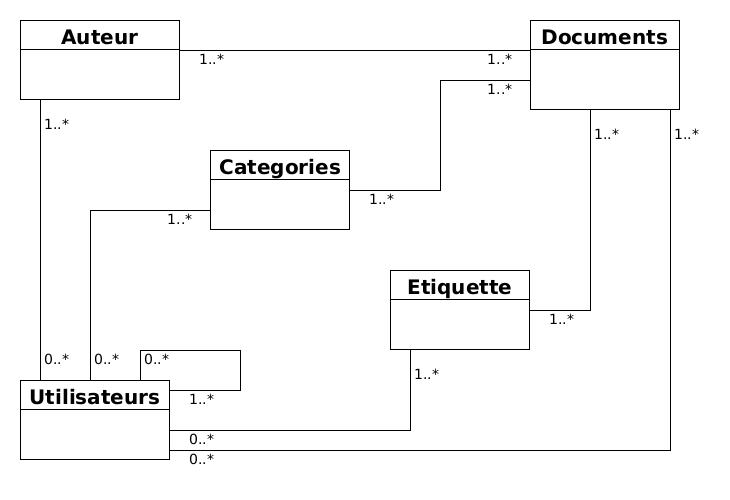
\includegraphics[width=0.75\linewidth]{Pictures/RelationEntreLesTables.jpg}
				\caption{Liens entre les relations}
				\label{RelationEntreTables}
			\end{figure}


			\paragraph{}Dans le mod\`ele de donn\'es relationnel, on cr\'ee un lien du type  plusieurs \`a plusieurs en ajoutant une nouvelle table qui recevra les cl\'es primaires des relations \`a relier comme cl\'es \'etrang\`eres. Par cons\'equent, chacun de ces liens va donner naissance \`a une nouvelle table. Ainsi, nous cr\'eerons huit nouvelles tables qui peuvent \^etre r\'eparties en deux groupes suivant les champs qui les composent:% Toutefois, \'etant donn\'e que tous , nous avons d\'ecid\'e de les unir en une seule relation nomm\'ee \textit{Gestion}. Pour les m\^emes raisons, les autres tables sont unies pour former la table tableRelation.

			\paragraph{}Nous obtenons ainsi les relations suivantes:


			\subsubsection*{Les tables de gestion}
				Les tables des liens entre la relation Utilisateur et les autres auront rigoureusement les m\^emes champs:

				\begin{tabularx}{500pt}{>{- }m{4cm} X}
					\textit{ IdentifiantAdmin \newline(Cl\'e \'etrang\`ere) \newline(Cl\'e primaire)} & Code permettant d'identifier l'administrateur qui a effectu\'e le changement. \\
					\textit{ IdentifiantXxxx \newline(Cl\'e \'etrang\`ere) \newline(Cl\'e primaire)} & Code permettant d'identifier l'\'el\'ement qui a subit le changement.  \\
					\textit{Date} & Date \`a laquelle le changement a \'et\'e effectu\'e. \\
					\textit{TypeGestion} & Pr\'ecise s'il s'agit d'un ajout, d'une suppression, ... \\
				\end{tabularx}
				\vspace{.5cm}


			\subsubsection*{Les tables de liaison}
				Les tables qui lient la table tableDocuments aux autres tables (Except\'e tableUtilisateurs) ont aussi les m\^emes champs: \\

				\begin{tabularx}{500pt}{>{- }m{4cm} X}

					\textit{ idDocument \newline(Cl\'e \'etrang\`ere) \newline(Cl\'e primaire)} & Code permettant d'identifier le document li\'e. \\

					\textit{ idXxxx \newline(Cl\'e \'etrang\`ere) \newline(Cl\'e primaire)} & Code permettant d'identifier un enregistrement dans une autre table auquel le document est li\'e.\\
				\end{tabularx}

			\subsubsection*{Autres tables}
				L'impl\'ementation de la fonction de recherche, telle que nous la concevons, requiert l'utilisation de deux autres tables.

				\paragraph{} \textbf{Stopwords}\\
				Pour stocker nos Stopwords\footnote{Fonctionnalit\'e de mariadb. Il s'agit d'une liste de mot qui seront ignor\'e lors des recherches pour cause qu'ils sont consid\'er\'e comme d\'enu\'e de sens propre (Voir \href{https://mariadb.com/kb/en/full-text-index-stopwords/}{Mariadb Stopwords})} personnalis\'es dans le serveur.

				\begin{tabularx}{500pt}{>{- }m{4cm} X}

					\textit{ idMot\_d\_arret \newline(Cl\'e primaire)} & Code permettant d'identifier chaque enregistrement de fa\c{c}on unique. \\

					\textit{ Mot\_d\_arret} & Stopword.\\
				\end{tabularx}


				\paragraph{} \textbf{Dictionnaire}\\
				Pour stocker tous les mots utilis\'es dans la base de donn\'ees \`a l'excetption des stopwords.

				\begin{tabularx}{550pt}{>{- }m{4cm} X}

					\textit{ idMot \newline(Cl\'e primaire)} & Code permettant d'identifier chaque enregistrement de fa\c{c}on unique. \\

					\textit{ Mot } & Mot utilis\'e dans la base de donn\'ees.\\
				\end{tabularx}



		\subsection{Dictionnaire de donn\'ees}
			Le tableau~\ref{DictionnaireDeDonnees} pr\'esente la liste des relations \`a cr\'eer pour constituer la base de donn\'ees.
			\vspace{1cm}


            \begin{center}
			\begin{longtable}[c]{| m{0.22\linewidth}  m{0.3\linewidth}  m{0.16\linewidth}  m{0.22\linewidth} |}
%				\centering
                \caption{Dictionnaire de donn\'ees.} \label{DictionnaireDeDonnees} \\

					\hline
					\hline
					\rowcolor{TetTablo}
                    \textbf{\textsc{\Large{Nom}}} & \textbf{\textsc{\Large{Code}}} & \textbf{\textsc{\Large{Type}}} & \textbf{\textsc{\Large{Note}}}\\
					\hline
					\hline
					\endfirsthead

					\hline
					\hline
					\rowcolor{TetTablo}
					\textbf{\textsc{\Large{Nom}}} & \textbf{\textsc{\Large{Code}}} & \textbf{\textsc{\Large{Type}}} & \textbf{\textsc{\Large{Note}}}\\
					\hline
					\hline
					\endhead

					\hline
					\endfoot

					\hline
					\hline
					\endlastfoot

					\rowcolor{mybrown}
					\multicolumn{4}{l}{tableDocuments}\\
					Identifiant & PK\_idDocument & INT & Non sign\'e, Non nul, Auto-incr\'ement\'e, cl\'e primaire\\
					Titre & TITRE & VARCHAR(255) & Non nul\\
					R\'esum\'e & RESUME & TEXT & \\
					Taille & TAILLE & INT & Non sign\'e\\
					Adresse du fichier & FICHIER & VARCHAR(255) & Non nul\\
					Nombre de consultation & NombreDeConsultations & DOUBLE & Non nul, Non sign\'e\\
					Nombre de partages  & NombreDePartages & DOUBLE & Non nul, Non sign\'e \\
					Type de fichier & TypeFichier & ENUM & Non nul\\
					Langue & LANGUE & ENUM & \\
					Note  & NOTE & FLOAT & Non sign\'e, Non nul\\
					Nombre de notes  & NombreNotes & DOUBLE & Non sign\'e, Non nul\\
					Cr\'eation & DateCreationDocument & DATE & Non nul\\
					Admin\_Cr\'eation & AuteurCreationDocument & VARCHAR(255) & Non nul\\
					Derni\`ere modification & DateModificationDocument & DATE & Non nul\\
					Admin\_Modification & AuteurModificationDocument & VARCHAR(255) & Non nul\\
					Supprim\'e & SupprimerDocument & BOOLEAN & Non nul\\

					\rowcolor{mybrown}
					\multicolumn{4}{l}{tableCategories} \\
					Identifiant & PK\_idCategorie & INT & Non sign\'e, Non nul, Auto-incr\'ement\'e, cl\'e primaire\\
					Cat\'egorie & CATEGORIE & VARCHAR(31) & Unique, Non nul\\
					Date de cr\'eation & DateCreationCategorie & DATE & Non nul\\
					Admin\_Cr\'eation & AuteurCreationCategorie & VARCHAR(255) & Non nul\\
					Date derni\`ere modification & DateModificationCategorie & DATE & Non nul\\
					Admin\_Modification & AuteurModificationCategorie & VARCHAR(255) & Non null\\
					Supprim\'e & SupprimerCategorie & BOOLEAN & Non nul\\

					\rowcolor{mybrown}
					\multicolumn{4}{l}{tableUtilisateurs} \\
					Identifiant & PK\_idUtil & INT & Non sign\'e, Non nul, Auto-incr\'ement\'e, cl\'e primaire\\
					Nom & NomUtil & VARCHAR(31) &  \\
					Pr\'enom  & PrenomUtil & VARCHAR(31) & \\
					Nom d'utilisateur  & USERNAME & VARCHAR(31) & Unique\\
					Addresse IP  & AddresseIP & VARCHAR(128) & \\
					E-mail & EmailUtil & VARCHAR(255) & \\
					Mot de passe & MotDePasseUtil & VARCHAR(255) & \\
					Administrateur & Administrateur & BOOLEAN & Non nul\\
					Date de cr\'eation & DateCreationUtil & DATE & Non nul\\
					Admin\_Cr\'eation & AuteurCreationUtil & VARCHAR(255) & Non nul\\
					Date derni\`ere modification & DateModificationUtil & DATE & Non nul\\
					Admin\_Modification & AuteurModificationUtil & VARCHAR(255) & Non nul\\
					Supprim\'e & SupprimerUtil & BOOLEAN & Non nul\\

					\rowcolor{mybrown}
					\multicolumn{4}{l}{tableEtiquettes} \\
					Identifiant & PK\_idEtiquette & INT & Non sign\'e, Non nul, Auto-incr\'ement\'e, cl\'e primaire\\
					\'Etiquette & ETIQUETTE & VARCHAR(31) & Unique, Non nul\\
					Date de cr\'eation & DateCreationEtiquette & DATE & Non nul\\
					Admin\_Cr\'eation & AuteurCreationEtiquette & VARCHAR(31) & Non nul\\
					Date derni\`ere modification & DateModificationEtiquette & DATE & Non nul\\
					Admin\_Modification & AuteurModificationEtiquette & VARCHAR(31) & Non nul\\
					Supprim\'e & SupprimerEtiquette & BOOLEAN & Non nul\\

					\rowcolor{mybrown}
					\multicolumn{4}{l}{tableAuteurs} \\
					Identifiant & PK\_idAuteur & INT & Non sign\'e, Non nul, Auto-Incr\'ement\'e, cl\'e primaire\\
					Nom & NomAuteur & VARCHAR(31) & \\
					Pr\'enom & PrenomAuteur & VARCHAR(31) & \\
					E-mail & EmailAuteur & VARCHAR(31) & \\
					Admin\_Cr\'eation & AuteurCreationAuteur & VARCHAR(255) & Non nul\\
					Date derni\`ere modification & DateModificationAuteur & DATE & Non nul\\
					Admin\_Modification & AuteurModificationAuteur & VARCHAR(255) & Non nul\\
					Supprim\'e & SupprimerAuteur & BOOLEAN & Non nul\\

					\rowcolor{mybrown}
					\multicolumn{4}{l}{tableDocumentAuteur} \\
					IdentifiantDocument & FK\_IdentifiantDocument & INT & Non sign\'e, Non nul, cl\'e \'etrang\`ere, cl\'e primaire\\
					IdentifiantAuteur & FK\_IdentifiantAuteur & INT & Non sign\'e, Non nul, cl\'e \'etrang\`ere, cl\'e primaire\\

					\rowcolor{mybrown}
					\multicolumn{4}{l}{tableDocumentCategorie} \\
					IdentifiantDocument & FK\_IdentifiantDocument & INT & Non sign\'e, Non nul, cl\'e \'etrang\`ere, cl\'e primaire\\
					IdentifiantCategorie & FK\_IdentifiantCategorie & INT & Non sign\'e, Non nul, cl\'e \'etrang\`ere, cl\'e primaire\\

					\rowcolor{mybrown}
					\multicolumn{4}{l}{tableDocumentEtiquette} \\
					IdentifiantDocument & FK\_IdentifiantDocument & INT & Non sign\'e, Non nul, cl\'e \'etrang\`ere, cl\'e primaire\\
					IdentifiantEtiquette & FK\_IdentifiantEtiquette & INT & Non sign\'e, Non nul, cl\'e \'etrang\`ere, cl\'e primaire\\

					\rowcolor{mybrown}
					\multicolumn{4}{l}{tableAdminAuteur} \\
					IdentifiantAdmin & FK\_IdentifiantAdmin & INT & Non sign\'e, Non nul, cl\'e \'etrang\`ere, cl\'e primaire\\
					IdentifiantAuteur & FK\_IdentifiantAuteur & INT & Non sign\'e, Non nul, cl\'e \'etrang\`ere, cl\'e primaire\\
					Date & DATE & TIMESTAMP & Non nul\\
					Types de gestion & TypeGestion & ENUM & \\

					\rowcolor{mybrown}
					\multicolumn{4}{l}{tableAdminDocument} \\
					IdentifiantAdmin & FK\_IdentifiantAdmin & INT & Non sign\'e, Non nul, cl\'e \'etrang\`ere, cl\'e primaire\\
					IdentifiantDocument & FK\_IdentifiantDocument & INT & Non sign\'e, Non nul, cl\'e \'etrang\`ere, cl\'e primaire\\
					Date & DATE & TIMESTAMP & Non nul\\
					Types de gestion & TypeGestion & ENUM & \\

					\rowcolor{mybrown}
					\multicolumn{4}{l}{tableAdminCategorie} \\
					IdentifiantAdmin & FK\_IdentifiantAdmin & INT & Non sign\'e, Non nul, cl\'e \'etrang\`ere, cl\'e primaire\\
					IdentifiantCategorie & FK\_IdentifiantCategorie & INT & Non sign\'e, Non nul, cl\'e \'etrang\`ere, cl\'e primaire\\
					Date & DATE & TIMESTAMP & Non nul\\
					Types de gestion & TypeGestion & ENUM & \\

					\rowcolor{mybrown}
					\multicolumn{4}{l}{tableAdminUtilisateur} \\
					IdentifiantAdmin & FK\_IdentifiantAdmin & INT & Non sign\'e, Non nul, cl\'e \'etrang\`ere, cl\'e primaire\\
					IdentifiantUtilisateur & FK\_IdentifiantUtilisateur & INT & Non sign\'e, Non nul, cl\'e \'etrang\`ere, cl\'e primaire\\
					Date & DATE & TIMESTAMP & Non nul\\
					Types de gestion & TypeGestion & ENUM & \\

					\rowcolor{mybrown}
					\multicolumn{4}{l}{tableAdminEtiquette} \\
					IdentifiantAdmin & FK\_IdentifiantAdmin & INT & Non sign\'e, Non nul, cl\'e \'etrang\`ere, cl\'e primaire\\
					IdentifiantEtiquette & FK\_IdentifiantEtiquette & INT & Non sign\'e, Non nul, cl\'e \'etrang\`ere, cl\'e primaire\\
					Date & DATE & TIMESTAMP & Non nul\\
					Types de gestion & TypeGestion & ENUM & \\

					\rowcolor{mybrown}
					\multicolumn{4}{l}{Dictionnaire} \\
					Identifiant & idMot & INT & Non sign\'e, Non nul, Auto-Increment, cl\'e primaire\\
					Mot & Mot & VARCHAR(31) & Unique, Non nul\\

					\rowcolor{mybrown}
					\multicolumn{4}{l}{Stopwords} \\
					Identifiant & idMot\_d\_arret & INT & Non sign\'e, Non nul, Auto-incr\'ement\', cl\'e primaire\\
					IdentifiantEtiquette & FK\_IdentifiantEtiquette & VARCHAR(31) & Unique, Non nul\\
			\end{longtable}
           \end{center}


%
%
%			\section{Vue}
%				Une vue\cite{VueSQL} est une relation SQL qui n'existe pas sur la m\'emoire mais est d\'efinie par une requ\^etes sur les tables existantes dans la base. Elles permettent au syst\`eme de tra\^iter un ensemble de donn\'ees extraites d'une ou ou de plusieurs relation comme s'il s'agissait d'une seule table sans, pour autant, solliciter la quantit\'e de ressource qu'il faudrait au serveur SQL pour g\'erer une table.\\
%				Nous cr\'eons les vues suivantes.
%				\vspace{.5cm}
%
%
%
%
%
%				\subsubsection*{Gestion}
%				Cette relation est cr\'e\'ee \`a travers les tables de gestion. La vue gestion ainsi cr\'e\'ee contient la liste de toutes les op\'erations CRUD\footnote{Cr\'eation, Lecture, Mise \`a jour, Suppression} \'effectu\'ee sur la base. Elle contient les champs suivants:
%
%				\begin{tabularx}{500pt}{>{- }m{4cm} X}
%					\textit{ IdGestion \newline(Cl\'e primaire)} &  Code permettant d'identifier un enregistrement de fa\c{c}on unique dans la base de donn\'ees. \\
%					\textit{ IdUtilisation \newline(Cl\'e \'etrang\`ere)} & Code permettant d'identifier l'administrateur qui a effectu\'e le changement. \\
%					\textit{ IdEnregistrement \newline(Cl\'e \'etrang\`ere)} & Code permettant d'identifier l'\'el\'ement qui a subit le changement.  \\
%					\textit{TypeGestion} & Pr\'ecise s'il s'agit d'un ajout, d'une suppression, ... \\
%					\textit{RelationAGerer} & Nom de la relation qui a subit le changement\\
%					\textit{DateGestion} & Date \`a laquelle le changement a \'et\'e effectu\'e. \\
%				\end{tabularx}
%
%
%
%			\subsubsection*{Documents}
%				La vue Document est cr\'e\'ee \`a travers les tables \textbf{tableEtiquettes}, \textbf{tableAuteurs}, \textbf{tableCategories}, leurs tables de liaisons avec tableDocuments et la table \textbf{tableDocuments} elle m\^eme. Chaque enregistrement de la relation \textbf{Documents} contient toutes les donn\'ees d\'efinissant une des documents que le projet veut rendre accessible. La vue \textbf{Documents} est l'impl\'ementation de la relation du m\^eme nom cens\'e contenir les informations concernant les documents \`a distribuer via le syst\`eme (Voir Section~\ref{SectionRelationDocuments}).



			\section{Triggers}
			 	Un trigger\cite{TriggerSQL} est une contrainte SQL qui d\'efini un ensemble d'actions qui doivent \^etre effectu\'e \`a l'occurrence d'un certain \'ev\`enement et sous certaines conditions.\\
			 	Nous en faisons usage, ici, pour effectuer certains t\^aches.  Ces triggers peuvent \^etre divis\'es en deux groupes comme suit:

				 	\begin{tabularx}{500pt}{m{.25\linewidth} X X}
				 		\rowcolor{lightgray}
				 		\textbf{ \textsc{Libell\'e}} & \textbf{ \textsc{\'Ev\`enement d'occurence}} & \textbf{ \textsc{Action}}\\
				 		\hline
				 		\hline

				 		\textit{ trgEnregistrerXxxx} & Apr\`es la r\'ealisation d'un op\'eration CRUD & Enregistrer l'op\'eration en question dans la relation \textbf{Gestion} \\


				 		\textit{ tgrRemplirDicoXxxx} & Apr\`es qu'un ajout ou une modification ait \'et\'e effectu\'e sur une des tables tableDocuments, tableAuteurs et tableEtiquettes & Enregistrer, dans la table Dictionnaire, les nouveaux mots utilis\'es pour les champs concern\'es par la fonction de recherche \\

				 	\end{tabularx}



 	\section{Proc\'edures}
		 Nous utilisons une proc\'edures pour permettre au serveur d'application la possibilit\'e de rechercher des documents dans la base.


		\begin{tabularx}{500pt}{m{.25\linewidth} X}
			\rowcolor{lightgray}
			\textbf{ \textsc{Libell\'e}} & \textbf{ \textsc{Op\'eration}}\\
			\hline
			\hline

%			\textit{ajouterLangue} & Modifie la description de la relation tableDocuments et ajoute une nouvelle valeur possible pour le champ \textbf{Langue} qui, on le rappelle, est de type Enum.\\

%			\textit{ajouterType} & Modifie la description de la relation tableDocuments et ajoute une nouvelle valeur possible pour le champ \textbf{Type de fichier} qui, on le rapelle, est de type Enum.\\

			\textit{Rechercher} & S\'electionne tous les enregistrement de la relation \textbf{Documents} qui contient, int\'egralement ou partiellement, une ou plusieurs des mots des mots fournis en param\`etre.\\

		\end{tabularx}


	\section{Sch\'ema des donn\'ees}
		Le diagramme de la figure~\ref{SchemaDeDonnees} d\'ecrit la disposition des donn\'ees dans la base de donn\'ees construite.


			\begin{figure}[]
				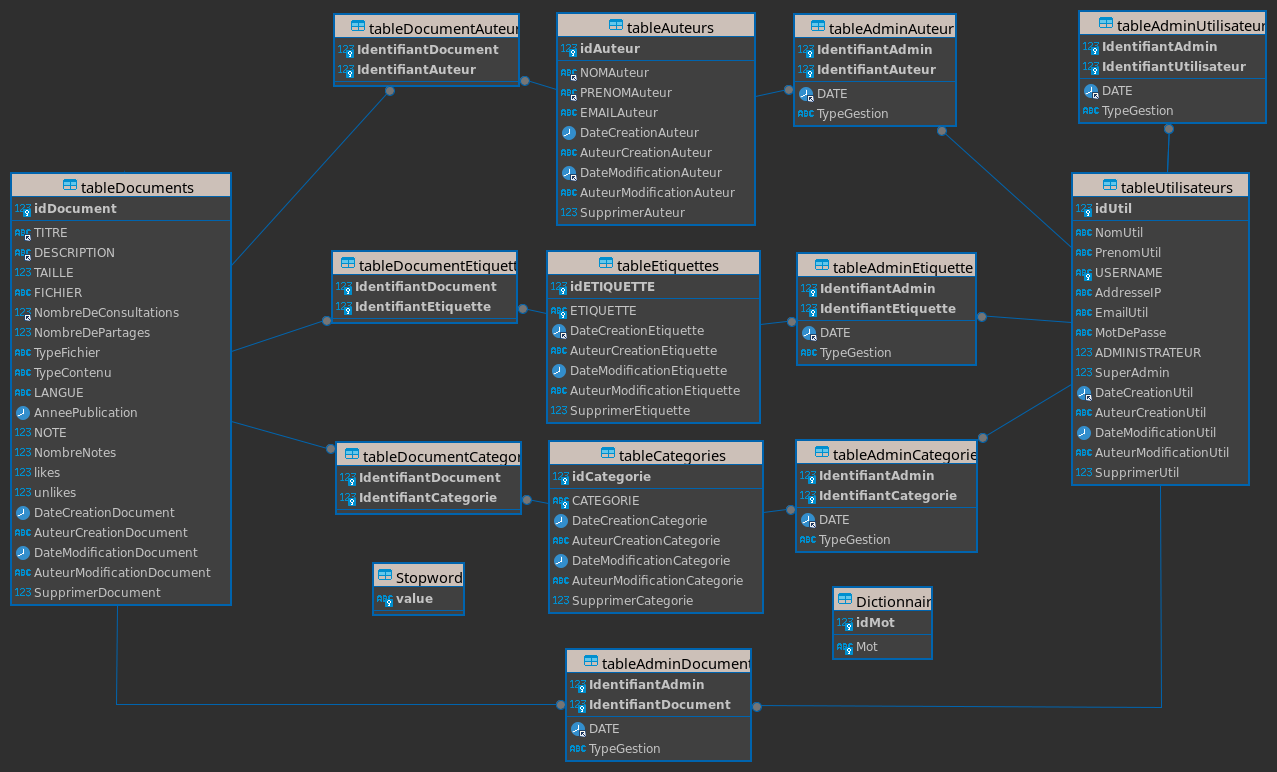
\includegraphics[width=0.8\textwidth]{Pictures/DiagrammeDeDonnees.png}
				\centering
				\caption{Sch\'ema des donn\'ees}
				\label{SchemaDeDonnees}
			\end{figure}

		\newrefsection
			\chapter{S\'ecurit\'e}

	\label{ChapSecurite}

	En informatique, s\'ecuriser c'est garantir la confidentialit\'e, l'int\'egrit\'e et la disposponibilit\'e des donn\'ees d'un syst\`eme en le prot\'egeant contre les manipulations et acc\`es non authoris\'es, les violations de donn\'ees ou tout autres activit\'es visant \`a compromettre son cadre de fonctionnement.

	\paragraph{} Le processus consiste, dans un premier temps, \`a identifier les vuln\'erabilt\'es du syst\`eme ainsi que les menaces qui posent sur lui. Puis, dans un second temps, \`a trouver des moyens qui permettent de prot\'eger efficacement le syst\`eme contre les menaces et de compenser ses vuln\'erabilit\'es. Et, dans un dernier \`a impl\'ementer la s\'ecurit\'e.

	\section{OWASP Application Security Verification Standard}
		Les menaces et vuln\'erabilit\'es d'un site Web sont nombreuses. Si bien qu'il devient difficile de faire une liste compl\`ete et exhaustives de tous les types d'attaques qu'un site Web pourrait subir et de tout ce qui represente une vuln\'erabilit\'e pour le site. Heureusement, l'organisation {\itshape Open Worldwide Application Security Project \bfseries(OWASP)} a produit le standard ASVS pour aider \`a la s\'ecurit\'e des applications Web.

		\paragraph{} Le standard ASVS (Application Security Verification Standard) est une liste d'exigences concernant la s\'ecurit\'e fonctionnel et non-fonctionnel requis dans la construction de sites Webs. Le standard est divis\'e de fa\c{c}on modulaire en 14 chapitres qui ont chacun leur objectifs sp\'ecifiques concernant un ou plusieurs aspects de la s\'ecurit\'e de l'application.

		\paragraph{} \`A travers ASVS, LeS travaux d'{\bfseries identifaction des menaces et vuln\'erabilit\'es} des sites et de {\bfseries conception de moyens de d\'efenses efficaces pour se prot\'eger contre le menaces et pour compenser les vuln\'erabilit\'es} sont donc d\'ej\`a effectu\'e et sont r\'evis\'es reguli\`erement par une communaut\'e comp\'etente et exp\'eriment\'ee en la mati\`ere. Il ne nous reste plus qu'\`a biens les utiliser pour s\'ecuriser notre site Web.

	\section{Impl\'ementation}
		Ainsi donc, en plus des m\'ethodes des spring boot pour contribuer \`a la s\'ecurit\'e des applications, nous utiliserons \textbf{ASVS 4.0.3} comme un framework qui d\'efini les t\^aches sp\'ecifiques que nous devons impl\'ementer pour avoir un produit s\'ecuris\'e. Pendant l'impl\'ementation de chacun des diff\'erentes structures constituants l'application, nous prenons en compte les consignes de \textbf{ASVS 4.0.3} sur l'impl\'ementation de la  struture en question pour nous assurer qu'elle soit construite et utilis\'ee de fa\c{c}on s\'ecuris\'ee.


%
%		Toutefois, pour ne pas d\'eborder du temps imparti, nous nous basons sur les objectifs de chacun des chapitre qui sont fournis dans la documentation du standard pour identifier les impl\'ementations qui sont significatives pour le projet. Ainsi nous avons s\'electionn\'e les suivants:
%				\begin{itemize}
%					\item[-] Authentification
%					\item[-] Validation des entr\'ees
%					\item[-] Protection des donn\'ees
%					\item[-] S\'ecurit\'e de la communication
%					\item[-] Codes malveillants
%				\end{itemize}
%
%			\paragraph{}En suite, nous filtrons \`a nouveau pour \'eliminer certains contr\^oles qui ne collent pas avec notre application comme, par exemple, v4.0.3-2.8.7 concerne les donn\'ees biom\'etriques, or nous n'en utilisons pas.\\
%			La liste compl\`ete des exigences satisfaites est pr\'esent\'ees ci-apr\`es'.
%
%		\begin{center}
%			\
%			\begin{longtable}{ >{\centering\arraybackslash\bfseries}m{0.2\textwidth} >{\raggedright\arraybackslash}m{0.05\textwidth} >{\raggedright\arraybackslash}m{0.68\textwidth}}
%				\caption{Liste des exigences impl\'ement\'ees sur \projectName} \\
%
%				\hline
%				\hline
%				\rowcolor{TetTablo}
%				\textbf{\textsc{\large{Area}}} & \textbf{\textsc{\large{\hfill \# \hfill}}} & \textbf{\textsc{\large{\hspace*{80pt} Requirement }}}\\
%				\hline
%				\hline
%				\endfirsthead
%
%				\hline
%				\hline
%				\rowcolor{TetTablo}
%				\textbf{\textsc{\large{Area}}} & \textbf{\textsc{\large{\hfill \# \hfill}}} & \textbf{\textsc{\large{\hspace*{80pt} Requirement}}}\\
%				\hline
%				\hline
%				\endhead
%
%				\hline
%				\endfoot
%
%				\hline
%				\hline
%				\endlastfoot
%
%				\hline
%				\rowcolor{mybrown}
%				\multicolumn{3}{c}{Authentication}\\
%				\hline
%				Password Security  & 2.1.1 & Verify that user set passwords are at least 12 characters in length (after multiple spaces are combined).\\
%				& 2.1.2 & Verify that passwords of at least 64 characters are permitted, and that passwords of more than 128 characters are denied.\\
%				& 2.1.3 & Verify that password truncation is not performed. However, consecutive multiple spaces may be replaced by a single space.\\
%				& 2.1.4 & Verify that any printable Unicode character, including language neutral characters such as spaces and Emojis are permitted in passwords. \\
%				& 2.1.5 & Verify users can change their password. \\
%				& 2.1.6 & Verify that password change functionality requires the user's current and new password. \\
%				& 2.1.7 & Verify that passwords submitted during account registration, login, and password change are checked against a set of breached passwords either locally (such as the top 1,000 or 10,000 most common passwords which match the system's password policy) or using an external API. If using an API a zero knowledge proof or other mechanism should be used to ensure that the plain text password is not sent or used in verifying the breach status of the password. If the password is breached, the application must require the user to set a new non-breached password.\\
%				& 2.1.8 & Verify that a password strength meter is provided to help users set a stronger password. \\
%				& 2.1.9 & Verify that there are no password composition rules limiting the type of characters permitted. There should be no requirement for upper or lower case or numbers or special characters.\\
%				& 2.1.10 & Verify that there are no periodic credential rotation or password history requirements. \\
%				& 2.1.11 & Verify that "paste" functionality, browser password helpers, and external password managers are permitted. \\
%				& 2.1.12 & Verify that the user can choose to either temporarily view the entire masked password, or temporarily view the last typed character of the password on platforms that do not have this as built-in functionality. \\
%				\hline
%
%				General Authenticator Security & 2.2.1 & Verify that anti-automation controls are effective at mitigating breached credential testing, brute force, and account lockout attacks. Such controls include blocking the most common breached passwords, soft lockouts, rate limiting, CAPTCHA, ever increasing delays between attempts, IP address restrictions, or risk-based restrictions such as location, first login on a device, recent attempts to unlock the account, or similar. Verify that no more than 100 failed attempts per hour is possible on a single account. \\
%				& 2.2.2 & Verify that the use of weak authenticators (such as SMS and email) is limited to secondary verification and transaction approval and not as a replacement for more secure authentication methods. Verify that stronger methods are offered before weak methods, users are aware of the risks, or that proper measures are in place to limit the risks of account compromise. \\
%				& 2.2.3 & Verify that secure notifications are sent to users after updates to authentication details, such as credential resets, email or address changes, logging in from unknown or risky locations. The use of push notifications - rather than SMS or email - is preferred, but in the absence of push notifications, SMS or email is acceptable as long as no sensitive information is disclosed in the notification. \\
%				\hline
%
%				Authenticator Lifecycle & 2.3.1 & Verify system generated initial passwords or activation codes SHOULD be securely randomly generated, SHOULD be at least 6 characters long, and MAY contain letters and numbers, and expire after a short period of time. These initial secrets must not be permitted to become the long term password. \\
%				& 2.3.2 & Verify that enrollment and use of user-provided authentication devices are supported, such as a U2F or FIDO tokens. \\
%				& 2.3.3 & Verify that renewal instructions are sent with sufficient time to renew time bound authenticators. \\
%				\hline
%
%				Credentials Storage & 2.4.1 & Verify that passwords are stored in a form that is resistant to offline attacks. Passwords SHALL be salted and hashed using an approved one-way key derivation or password hashing function. Key derivation and password hashing functions take a password, a salt, and a cost factor as inputs when generating a password hash.\\
%				& 2.4.2 & Verify that the salt is at least 32 bits in length and be chosen arbitrarily to minimize salt value collisions among stored hashes. For each credential, a unique salt value and the resulting hash SHALL be stored.\\
%				& 2.4.3 & Verify that if PBKDF2 is used, the iteration count SHOULD be as large as verification server performance will allow, typically at least 100,000 iterations.\\
%				& 2.4.4 & Verify that if bcrypt is used, the work factor SHOULD be as large as verification server performance will allow, with a minimum of 10.\\
%				& 2.4.5 & Verify that an additional iteration of a key derivation function is performed, using a salt value that is secret and known only to the verifier. Generate the salt value using an approved random bit generator [SP 800-90Ar1] and provide at least the minimum security strength specified in the latest revision of SP 800-131A. The secret salt value SHALL be stored separately from the hashed passwords (e.g., in a specialized device like a hardware security module). \\
%				\hline
%
%				Credential Recovery  & 2.5.1 & Verify that a system generated initial activation or recovery secret is not sent in clear text to the user.\\
%				& 2.5.2 & Verify password hints or knowledge-based authentication (so-called "secret questions") are not present. \\
%				& 2.5.3 & Verify password credential recovery does not reveal the current password in any way.\\
%				& 2.5.4 & Verify shared or default accounts are not present (e.g. "root", "admin", or "sa"). \\
%				& 2.5.5 & Verify that if an authentication factor is changed or replaced, that the user is notified of this event. \\
%				& 2.5.6 & Verify forgotten password, and other recovery paths use a secure recovery mechanism, such as time-based OTP (TOTP) or other soft token, mobile push, or another offline recovery mechanism.\\
%				& 2.5.7 & Verify that if OTP or multi-factor authentication factors are lost, that evidence of identity proofing is performed at the same level as during enrollment. \\
%				\hline
%
%				Look-up Secret Verifier  & 2.6.1 & Verify that lookup secrets can be used only once. \\
%				& 2.6.2 & Verify that lookup secrets have sufficient randomness (112 bits of entropy), or if less than 112 bits of entropy, salted with a unique and random 32-bit salt and hashed with an approved one-way hash. \\
%				& 2.6.3 & Verify that lookup secrets are resistant to offline attacks, such as predictable values. \\
%				\hline
%
%				Out of Band Verifier & 2.7.1 & Verify that clear text out of band (NIST "restricted") authenticators, such as SMS or PSTN, are not offered by default, and stronger alternatives such as push notifications are offered first. \\
%				& 2.7.2 & Verify that the out of band verifier expires out of band authentication requests, codes, or tokens after 10 minutes. \\
%				& 2.7.3 & Verify that the out of band verifier authentication requests, codes, or tokens are only usable once, and only for the original authentication request. \\
%				& 2.7.4 & Verify that the out of band authenticator and verifier communicates over a secure independent channel. \\
%				& 2.7.5 & Verify that the out of band verifier retains only a hashed version of the authentication code. \\
%				& 2.7.6 & Verify that the initial authentication code is generated by a secure random number generator, containing at least 20 bits of entropy (typically a six digital random number is sufficient). \\
%				\hline
%
%				One Time Verifier & 2.8.1 & Verify that time-based OTPs have a defined lifetime before expiring. \\
%				& 2.8.2 & Verify that symmetric keys used to verify submitted OTPs are highly protected, such as by using a hardware security module or secure operating system based key storage. \\
%				& 2.8.3 & Verify that approved cryptographic algorithms are used in the generation, seeding, and verification of OTPs. \\
%				& 2.8.4 & Verify that time-based OTP can be used only once within the validity period. \\
%				& 2.8.5 & Verify that if a time-based multi-factor OTP token is re-used during the validity period, it is logged and rejected with secure notifications being sent to the holder of the device. \\
%				& 2.8.6 & Verify physical single-factor OTP generator can be revoked in case of theft or other loss. Ensure that revocation is immediately effective across logged in sessions, regardless of location. \\
%				\hline
%
%				Cryptographic Verifier & 2.9.1 & Verify that cryptographic keys used in verification are stored securely and protected against disclosure, such as using a Trusted Platform Module (TPM) or Hardware Security Module (HSM), or an OS service that can use this secure storage. \\
%				& 2.9.2 & Verify that the challenge nonce is at least 64 bits in length, and statistically unique or unique over the lifetime of the cryptographic device. \\
%				& 2.9.3 & Verify that approved cryptographic algorithms are used in the generation, seeding, and verification. \\
%				Service Authentication  & 2.10.1 & Verify that intra-service secrets do not rely on unchanging credentials such as passwords, API keys or shared accounts with privileged access. \\
%				& 2.10.2 & Verify that if passwords are required for service authentication, the service account used is not a default credential. (e.g. root/root or admin/admin are default in some services during installation). \\
%				& 2.10.3 & Verify that passwords are stored with sufficient protection to prevent offline recovery attacks, including local system access. \\
%				& 2.10.4 & Verify passwords, integrations with databases and third-party systems, seeds and internal secrets, and API keys are managed securely and not included in the source code or stored within source code repositories. Such storage SHOULD resist offline attacks. The use of a secure software key store (L1), hardware TPM, or an HSM (L3) is recommended for password storage. \\
%
%				 \hline
%				 \rowcolor{mybrown}
%				 \multicolumn{3}{c}{Access Control}\\
%				 \hline
%
%				 General Access Control Design & 4.1.1 & Verify that the application enforces access control rules on a trusted service layer, especially if client-side access control is present and could be bypassed. \\
%				 & 4.1.2 & Verify that all user and data attributes and policy information used by access controls cannot be manipulated by end users unless specifically authorized. \\
%				 & 4.1.3 & Verify that the principle of least privilege exists - users should only be able to access functions, data files, URLs, controllers, services, and other resources, for which they possess specific authorization. This implies protection against spoofing and elevation of privilege.  \\
%				 & 4.1.5 & Verify that access controls fail securely including when an exception occurs.  \\
%				 \hline
%
%				 Operation Level Access Control & 4.2.1 & Verify that sensitive data and APIs are protected against Insecure Direct Object Reference (IDOR) attacks targeting creation, reading, updating and deletion of records, such as creating or updating someone else's record, viewing everyone's records, or deleting all records. \\
%				 & 4.2.2 & Verify that the application or framework enforces a strong anti-CSRF mechanism to protect authenticated functionality, and effective anti-automation or anti-CSRF protects unauthenticated functionality. \\
%				 \hline
%
%				 Other Access Control Considerations & 4.3.1 & Verify administrative interfaces use appropriate multi-factor authentication to prevent unauthorized use. \\
%				 & 4.3.2 & Verify that directory browsing is disabled unless deliberately desired. Additionally, applications should not allow discovery or disclosure of file or directory metadata, such as Thumbs.db, .DS\_Store, .git or .svn folders. \\
%				 & 4.3.3 & Verify the application has additional authorization (such as step up or adaptive authentication) for lower value systems, and / or segregation of duties for high value applications to enforce anti-fraud controls as per the risk of application and past fraud. \\
%
%				 \hline
%				 \rowcolor{mybrown}
%				 \multicolumn{3}{c}{Input Validation}\\
%				 \hline
%
%				 Input Validation  & 5.1.1 & Verify that the application has defenses against HTTP parameter pollution attacks, particularly if the application framework makes no distinction about the source of request parameters (GET, POST, cookies, headers, or environment variables). \\
%				 & 5.1.2 & Verify that frameworks protect against mass parameter assignment attacks, or that the application has countermeasures to protect against unsafe parameter assignment, such as marking fields private or similar.  \\
%				 & 5.1.3 & Verify that all input (HTML form fields, REST requests, URL parameters, HTTP headers, cookies, batch files, RSS feeds, etc) is validated using positive validation (allow lists).  \\
%				 & 5.1.4 & Verify that structured data is strongly typed and validated against a defined schema including allowed characters, length and pattern (e.g. credit card numbers, e-mail addresses, telephone numbers, or validating that two related fields are reasonable, such as checking that suburb and zip/postcode match).  \\
%				 & 5.1.5 & Verify that URL redirects and forwards only allow destinations which appear on an allow list, or show a warning when redirecting to potentially untrusted content. \\
%				 \hline
%
%				 Sanitization and Sandboxing  & 5.2.1 & Verify that all untrusted HTML input from WYSIWYG editors or similar is properly sanitized with an HTML sanitizer library or framework feature.  \\
%				 & 5.2.2 & Verify that unstructured data is sanitized to enforce safety measures such as allowed characters and length. \\
%				 & 5.2.3 & Verify that the application sanitizes user input before passing to mail systems to protect against SMTP or IMAP injection. \\
%				 & 5.2.4 & Verify that the application avoids the use of eval() or other dynamic code execution features. Where there is no alternative, any user input being included must be sanitized or sandboxed before being executed. \\
%				 & 5.2.5 & Verify that the application protects against template injection attacks by ensuring that any user input being included is sanitized or sandboxed. \\
%				 & 5.2.6 & Verify that the application protects against SSRF attacks, by validating or sanitizing untrusted data or HTTP file metadata, such as filenames and URL input fields, and uses allow lists of protocols, domains, paths and ports. \\
%				 & 5.2.7 & Verify that the application sanitizes, disables, or sandboxes user-supplied Scalable Vector Graphics (SVG) scriptable content, especially as they relate to XSS resulting from inline scripts, and foreignObject. \\
%				 & 5.2.8 & Verify that the application sanitizes, disables, or sandboxes user-supplied scriptable or expression template language content, such as Markdown, CSS or XSL stylesheets, BBCode, or similar. \\
%				 \hline
%
%				 Output encoding and Injection Prevention  & 5.3.1 & Verify that output encoding is relevant for the interpreter and context required. For example, use encoders specifically for HTML values, HTML attributes, JavaScript, URL parameters, HTTP headers, SMTP, and others as the context requires, especially from untrusted inputs\\
%				 & 5.3.2 & Verify that output encoding preserves the user's chosen character set and locale, such that any Unicode character point is valid and safely handled.  \\
%				 & 5.3.3 & Verify that context-aware, preferably automated - or at worst, manual - output escaping protects against reflected, stored, and DOM based XSS.  \\
%				 & 5.3.4 & Verify that data selection or database queries (e.g. SQL, HQL, ORM, NoSQL) use parameterized queries, ORMs, entity frameworks, or are otherwise protected from database injection attacks.  \\
%				 & 5.3.5 & Verify that where parameterized or safer mechanisms are not present, context-specific output encoding is used to protect against injection attacks, such as the use of SQL escaping to protect against SQL injection.  \\
%				 & 5.3.6 & Verify that the application protects against JSON injection attacks, JSON eval attacks, and JavaScript expression evaluation.  \\
%				 & 5.3.7 & Verify that the application protects against LDAP injection vulnerabilities, or that specific security controls to prevent LDAP injection have been implemented.  \\
%				 & 5.3.8 & Verify that the application protects against OS command injection and that operating system calls use parameterized OS queries or use contextual command line output encoding.  \\
%				 & 5.3.9 & Verify that the application protects against Local File Inclusion (LFI) or Remote File Inclusion (RFI) attacks. \\
%				 & 5.3.10 & Verify that the application protects against XPath injection or XML injection attacks.  \\
%				 \hline
%
%				 Memory, String and Unmanaged Code  & 5.4.1 & Verify that the application uses memory-safe string, safer memory copy and pointer arithmetic to detect or prevent stack, buffer, or heap overflows. \\
%				 & 5.4.2 & Verify that format strings do not take potentially hostile input, and are constant. \\
%				 \hline
%
%				 & 5.4.3 & Verify that sign, range, and input validation techniques are used to prevent integer overflows. \\
%				 Deserialization Prevention  & 5.5.1 & Verify that serialized objects use integrity checks or are encrypted to prevent hostile object creation or data tampering.  \\
%				 & 5.5.2 & Verify that the application correctly restricts XML parsers to only use the most restrictive configuration possible and to ensure that unsafe features such as resolving external entities are disabled to prevent XML eXternal Entity (XXE) attacks. \\
%				 & 5.5.3 & Verify that de-serialization of untrusted data is avoided or is protected in both custom code and third-party libraries (such as JSON, XML and YAML parsers). \\
%				 & 5.5.4 & Verify that when parsing JSON in browsers or JavaScript-based backends, JSON.parse is used to parse the JSON document. Do not use eval() to parse JSON. \\
%
%				\hline
%				\rowcolor{mybrown}
%				\multicolumn{3}{c}{Input Protection}\\
%				\hline
%
%				General Data Protection & 8.1.1 & Verify the application protects sensitive data from being cached in server components such as load balancers and application caches. \\
%				& 8.1.2 & Verify that all cached or temporary copies of sensitive data stored on the server are protected from unauthorized access or purged/invalidated after the authorized user accesses the sensitive data. \\
%				& 8.1.3 & Verify the application minimizes the number of parameters in a request, such as hidden fields, Ajax variables, cookies and header values. \\
%				& 8.1.4 & Verify the application can detect and alert on abnormal numbers of requests, such as by IP, user, total per hour or day, or whatever makes sense for the application. \\
%				& 8.1.5 & Verify that regular backups of important data are performed and that test restoration of data is performed. \\
%				& 8.1.6 & Verify that backups are stored securely to prevent data from being stolen or corrupted. \\
%				\hline
%
%				Client-side Data Protection & 8.2.1 & Verify the application sets sufficient anti-caching headers so that sensitive data is not cached in modern browsers. \\
%				& 8.2.2 &  Verify that data stored in browser storage (such as localStorage, sessionStorage, IndexedDB, or cookies) does not contain sensitive data. \\
%				& 8.2.3 & Verify that authenticated data is cleared from client storage, such as the browser DOM, after the client or session is terminated. \\
%				\hline
%
%				Sensitive Private Data & 8.3.1 & Verify that sensitive data is sent to the server in the HTTP message body or headers, and that query string parameters from any HTTP verb do not contain sensitive data. \\
%				& 8.3.2 & Verify that users have a method to remove or export their data on demand. \\
%				& 8.3.3 & Verify that users are provided clear language regarding collection and use of supplied personal information and that users have provided opt-in consent for the use of that data before it is used in any way. \\
%				& 8.3.4 & Verify that all sensitive data created and processed by the application has been identified, and ensure that a policy is in place on how to deal with sensitive data.  \\
%				& 8.3.5 & Verify accessing sensitive data is audited (without logging the sensitive data itself), if the data is collected under relevant data protection directives or where logging of access is required. \\
%				& 8.3.6 & Verify that sensitive information contained in memory is overwritten as soon as it is no longer required to mitigate memory dumping attacks, using zeroes or random data. \\
%				& 8.3.7 & Verify that sensitive or private information that is required to be encrypted, is encrypted using approved algorithms that provide both confidentiality and integrity.  \\
%				& 8.3.8 & Verify that sensitive personal information is subject to data retention classification, such that old or out of date data is deleted automatically, on a schedule, or as the situation requires. \\
%
%
%				\hline
%				\rowcolor{mybrown}
%				\multicolumn{3}{c}{Communication Security}\\
%				\hline
%
%				Client Communications Security  & 9.1.1 & Verify that TLS is used for all client connectivity, and does not fall back to insecure or unencrypted communications.  \\
%				& 9.1.2 & Verify using up to date TLS testing tools that only strong cipher suites are enabled, with the strongest cipher suites set as preferred. \\
%				& 9.1.3 & Verify that only the latest recommended versions of the TLS protocol are enabled, such as TLS 1.2 and TLS 1.3. The latest version of the TLS protocol should be the preferred option. \\
%				\hline
%
%				Server Communication Security  & 9.2.1 & Verify that connections to and from the server use trusted TLS certificates. Where internally generated or self-signed certificates are used, the server must be configured to only trust specific internal CAs and specific self-signed certificates. All others should be rejected. \\
%				& 9.2.2 & Verify that encrypted communications such as TLS is used for all inbound and outbound connections, including for management ports, monitoring, authentication, API, or web service calls, database, cloud, serverless, mainframe, external, and partner connections. The server must not fall back to insecure or unencrypted protocols. \\
%				& 9.2.3 & Verify that all encrypted connections to external systems that involve sensitive information or functions are authenticated. \\
%				& 9.2.4 & Verify that proper certification revocation, such as Online Certificate Status Protocol (OCSP) Stapling, is enabled and configured. \\
%				& 9.2.5 & Verify that backend TLS connection failures are logged. \\
%
%
%			\end{longtable}
%		\end{center}


		\newrefsection
			\chapter{D\'eploiement}


\begin{figure}[ht]
	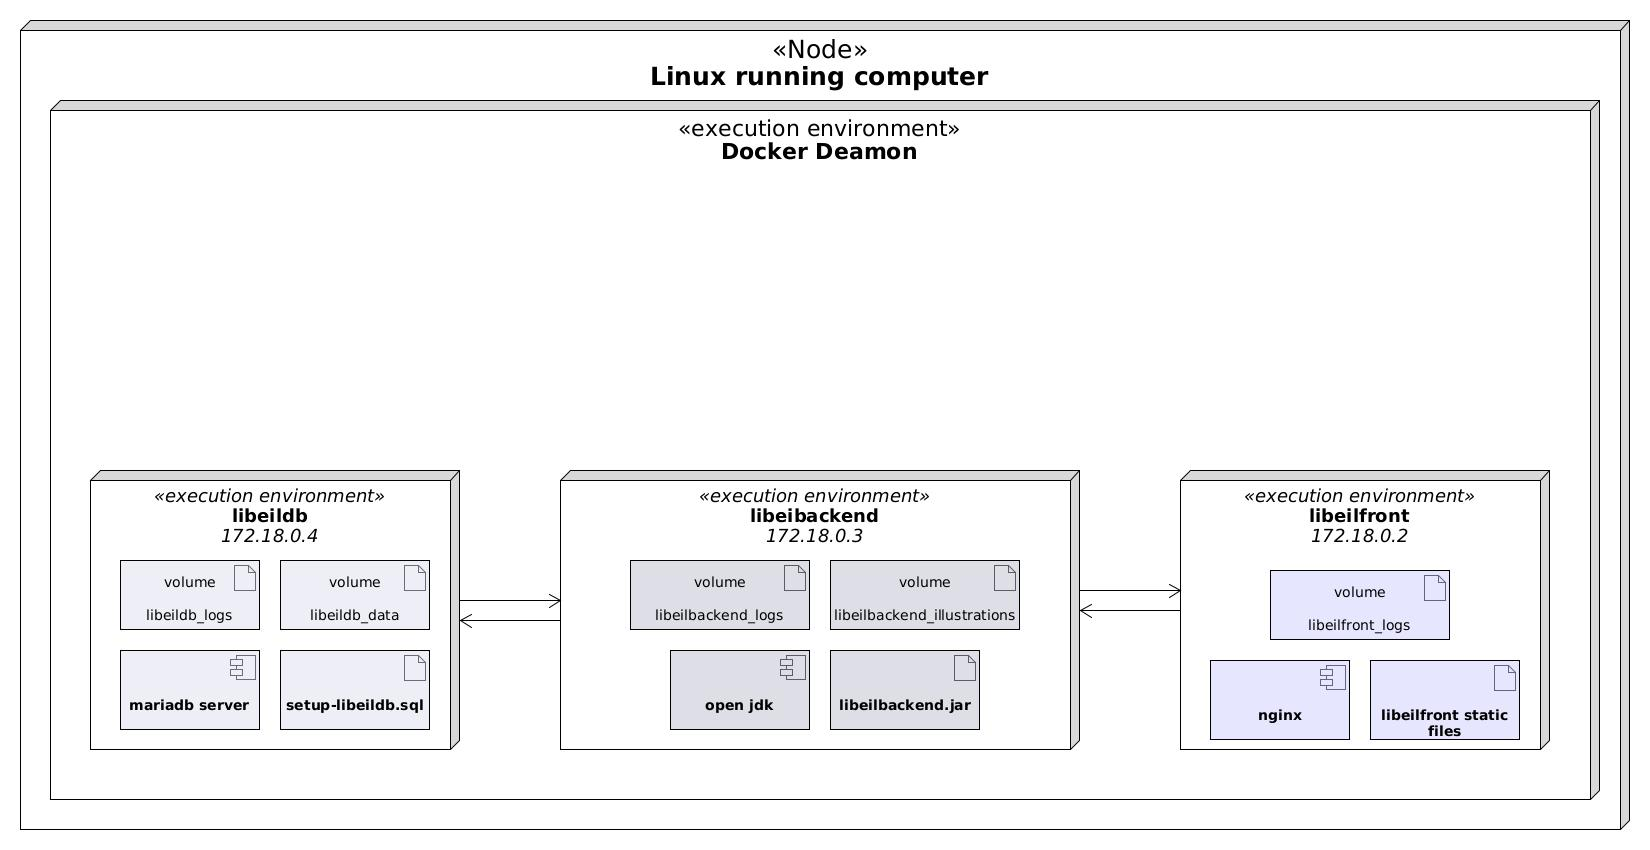
\includegraphics[width=0.75\textwidth]{Pictures/DiagrammeDeDeploiement.jpg}
	\centering
	\caption{Environnement de production.}
	\label{FigEnvironnementDeProduction}
\end{figure}

Le d\'eploiement est le processus qui, une fois la construction du site achet\'ee, permettra de la mettre en production. Dans notre cas, le d\'eploiement va consister \`a d\'efinir correctement l'environnement de production et \`a lancer les serveurs dans l'environnement d\'efini.


\section{Environnement de production}
\paragraph{} L'environnement de production d\'esigne ici l'ensemble form\'e d'un syst\`eme informatique qui fournit les ressources informatiques (Processeur, M\'emoire, Capacit\'e de stockage, ...) n\'ecessaires \`a l'ex\'ecution du site et d'une pile logicielle qui fournira les services dont le syst\`eme \`a besoin pour fonctionner (Syst\`eme d'exploitation, confidentialit\'e des donn\'ees, ...).

\subsection{Syst\`eme informatique}
Le syst\`eme informatique, suivant les besoins du site peut \^etre form\'e d'un ou de plusieurs ordinateurs et d'un ensemble de p\'eriph\'eriques.\\
Pour notre part, le syst\`eme informatique est un ordinateur physique ou virtuelle disposant d'assez de m\'emoire, d'espace de stockage, de d\'ebit r\'eseau, de CPU,... pour le fonctionnement de tout le site.


\subsection{Pile logicielle}
\subsubsection{Ubuntu}
Le premier logiciel est un syst\`eme d'exploitation. Nous utilisons Linux parce qu'en plus d'\^etre performant il est libre et open source par cons\'equent gratuit et fiable.

\paragraph{}De Linux, nous utilisons une distribution Ubuntu. Nous avons la derni\`ere version stable disponible.

\subsubsection{Docker Engine}
Docker est une technologie qui r\'evolutionne le d\'eveloppement et d\'eploiement de logiciels. Pour le d\'eploiement, Docker offre la possibilit\'e de lancer plusieurs applications sur un m\^eme ordinateur mais dans des environnements isol\'es les uns des autres.\\

L'application \textbf{Docker Engine} fournit une interface, et les service ad\'equates pour exploiter cette technologie.

\paragraph{} Nous utiliserons Docker pour pouvoir lancer les trois serveurs constituant le site sur un seul ordinateur.

\subsubsection{Nginx}
Pour assurer la disponibilit\'e de notre frontend sur le Web, nous devons utiliser un serveur Web. Les serveurs les plus connus et utilis\'es \`a cet effet sont \textbf{Apache} et \textbf{Nginx}.\\
Nous utilisons Nginx parce qu'il est plus efficace pour servir une front-end statique comme le notre et pour g\'erer une grande quantit\'e de trafique.







%\section{Protocole HTTPS}
%La s\'ecurit\'e du site est l'une des principales crit\`eres de qualit\'e de celui-ci. Elle consiste \`a garantir la disponibilit\'e, la confidentialit\'e et l'int\'egrit\'e des donn\'ees.\\ 
%HTTPS est une version s\'ecuris\'ee du protocole HTTP qui utilise SSL/TLS pour cripter les requ\^etes et r\'eponses HTTP classiques. Activer HTTPS sur le site le diminue les risques que les donne\'ees soient alt\'er\'ees au cours de leur transmission en contribuant ainsi \`a leur int\'egrit\'e. Cela emp\`eche qu'un hacker capte les paquets et d\'ecouvre acc\`ede au cr\'edential d'un administrateur et aux droit qui va avec. Donc il contribue \`a la confidentialit\'e des donn\'ees.			

%\paragraph{} Pour l'activer sur notre site, nous achetons un certificat SSL d'un vendeur et configurons Nginx pour utiliser le protocol s\'ecuris\'e de pr\'ef\'erence.


\section{Mise en production}
Une fois l'environnement de production op\'erationnel. Le site peut \^etre mis en production.

\subsection{Cr\'eation des images docker}
La premi\`ere \'etape consiste \`a cr\'eer une image docker pour chacun des trois serveurs.

\subsubsection{libeilfront}
L'image de l'interface utilisateur est bas\'ee sur la derni\`ere version alpine LTS (Long Time Support) du serveur web Nginx, \textbf{nginx:1.25.5-alpine}. On y cr\'ee un utilisateur non-root et un nouveau groupe pour notre utilisateur en sorte que Nginx ne soit pas lanc\'e en tant qu'administrateur, ce qui repr\'esenterait un risque pour la s\'ecurit\'e du site. Enfin on y copie les fichiers statiques provenant de l'application front-end d\'evelopp\'ee sur angular.

\subsubsection{libeilbackend}
L'image du serveur d'application est bas\'ee sur \textbf{openjdk:19-jdk-alpine}. On y cr\'ee un utilisateur non-root et un nouveau groupe pour notre utilisateur. Ensuite on y copie le package JAR (\textit{libeilbackend.jar}) de l'application d\'evelopp\'ee avec Spring Boot.

\subsubsection{libeildb}
L'image de la base de donn\'ees est bas\'ee sur \textbf{mariadb:10.11.6}. On y copie le script libeildb-setup.sql pour assurer la cr\'eation de la base une fois l'image lanc\'ee.

\subsection{Docker compose}
Docker compose permet de lancer les trois images comme une seule application. Pour cela nous cr\'eons un service pour chaque serveur bas\'e sur l'image ad\'equat. Nous cr\'eons aussi un r\'eseau priv\'e auquel nous ajoutons tous les services tout en leur donnant une adresse sur le r\'eseau priv\'e. En dernier lieu nous d\'efinissons des volumes pour garantir la persistance \`a la fois des donn\'ees de la base et des fichiers d'une part, et pour monter des fichiers de configuration aux conteneurs des diff\'erents services.\\

\subsection{+}
De l\`a, il suffit de lancer le fichier docker-compose.yml et l'application est en production






	\part*{Conclusion}

			\chapter{Guide d'utilisation}
	\paragraph{} Apr\`es d\'eveloppement et d\'eploiement de notre solution, le site web \projectName\ fournira l'acc\`es aux illustrations de l'URG\'eo comme d\'ecrit ci-apr\`es. 
	
	\section{G\'erer les illustrations sur le site}
	 L'enregistrement des illustrations sur le site passe par l'ensemble des \'etapes interm\'ediares suivantes:
		 	\begin{itemize}
		 		\item[-] G\'erer des administrateurs
		 		\item[-] G\'erer des cat\'egories
		 		\item[-] G\'erer des \'etiquettes
		 		\item[-] G\'erer des auteurs
		 		\item[-] G\'erer des documents
		 		\item[-] G\'erer les listes de choix
		 	\end{itemize} 
	 	
	 	\paragraph{} Ces travaux ne peuvent \^etre r\'ealis\'es que par un utilisateur avec les droits d'administrateurs. Avant tout, l'utilisateur doit se connecter sur le dashboard comme suit.
	 	
		\subsection{Authentification}
			\fcolorbox{frameblue}{fillblue}{
				\begin{minipage}{6in}
					\begin{itemize}
						\item[-] Naviguer vers l'URL de la page de connection du dashboard(Voir Figure~\ref{FigLoginPage}) :\dashboardURL\
						\item[-] Entrer son nom d'utilisateur
						\item[-] Entrer son mot-de-passe
						\item[-] Cliquer sur le bouton 
\includegraphics[height=2ex]{Pictures/BoutonLogin.png} pour se connecter sur le dashboard(Voir Figure~\ref{FigDashboardRoot})
					\end{itemize}
				\end{minipage}
			}
		
				
		\begin{figure}
			\centering
			\begin{minipage}{0.45\textwidth}
				\centering
				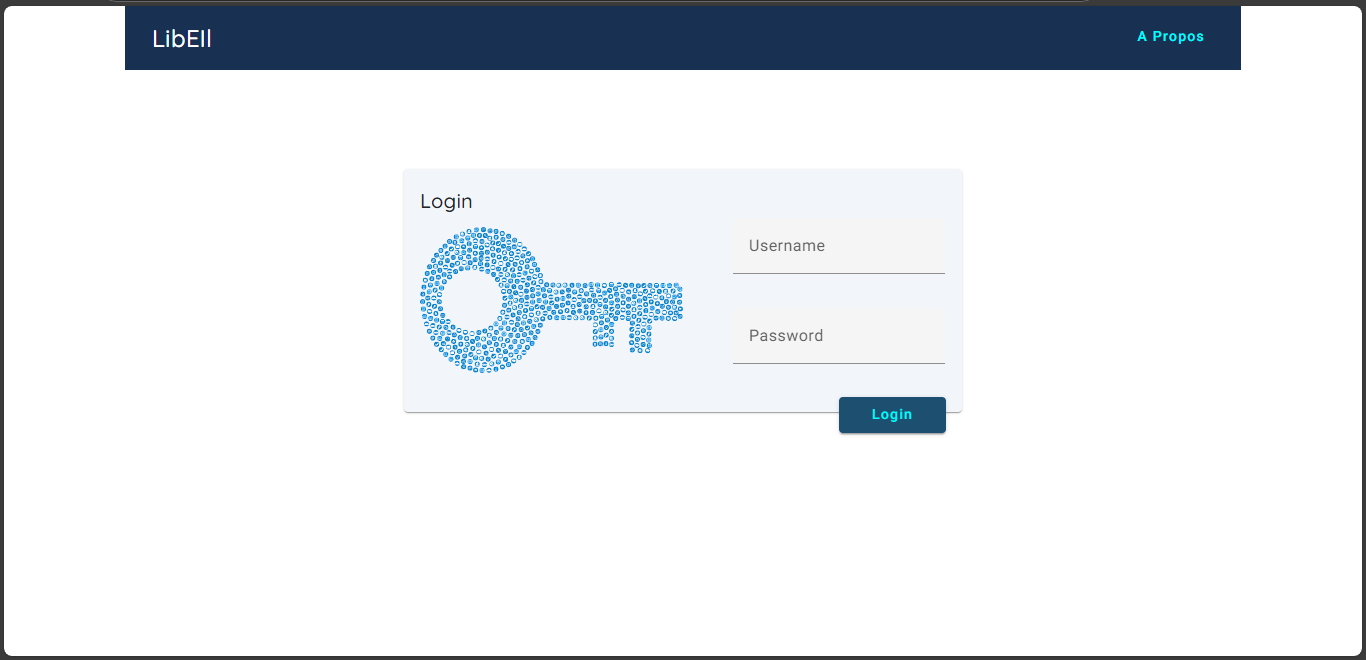
\includegraphics[width=\textwidth]{Pictures/PageDeConnection.png}
				\caption{Page de connection au dashboard}
				\label{FigLoginPage}
			\end{minipage}
			\hspace{5pt}
			\begin{minipage}{0.45\textwidth}
				\centering
				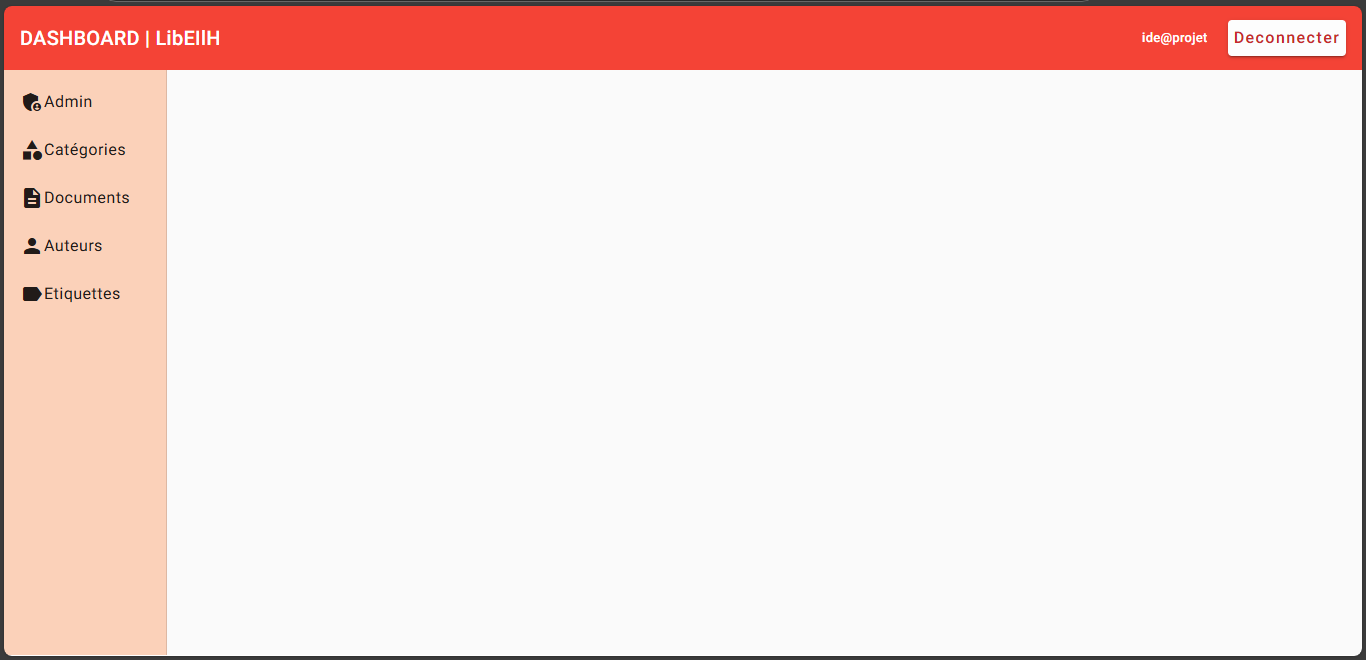
\includegraphics[width=\textwidth]{Pictures/Dashboard_rootPage.png}
				\caption{Page d'entr\'ee du dashboard}
				\label{FigDashboardRoot}
			\end{minipage}
		\end{figure}
		
		
		\paragraph{} Une fois connect\'e, l'administrateur choisit, dans la partie gauche de l'\'ecran, l'\'el\'ement \`a g\'erer.
		
		\begin{figure}[!ht]
			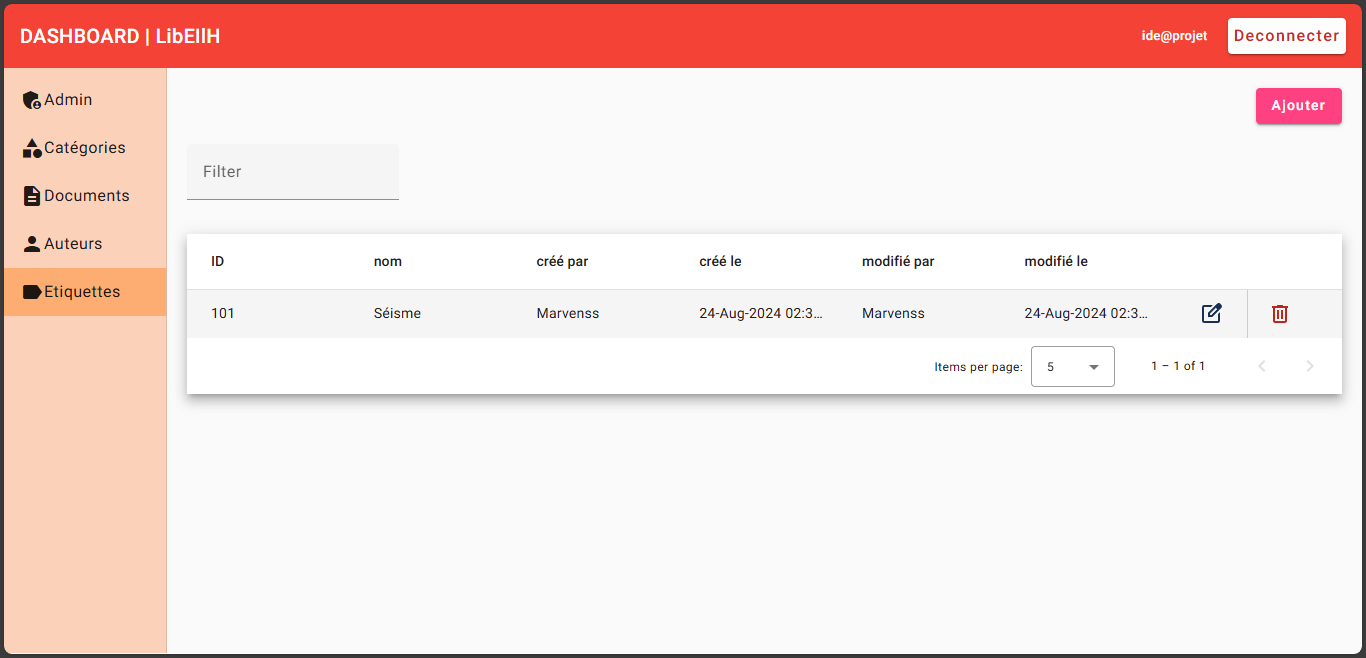
\includegraphics[width=0.5\textwidth]{Pictures/Dashboard_Etiquette.png}
			\centering
			\caption{Page de gestion des \'etiquettes}
			\label{FigChoixTypeElement}
		\end{figure}
		
		\paragraph{} Apr\`es avoir fait son choix (Voir Figure~\ref{FigChoixTypeElement}), l'utilisateur voit s'afficher la liste de tous les enregistrements de ce type dans la base de donn\'ees. Depuis cette page il est possible de supprimer ou modifier un enregistrement existant ou bien en ajouter un nouveau comme suit.
		
		\subsection{Ajouter}
			\fcolorbox{frameblue}{fillblue}{
				\begin{minipage}{6in}
					\begin{itemize}
						\item[-] Choisir le type d'\'el\'ement \`a ajouter 
						\item[-] Cliquer sur le bouton \includegraphics[height=2ex]{Pictures/BoutonAjouter.png} en haut \`a droite de l'\'ecran d'affichage
						\item[-] Remplir le formulaire d'ajout (Voir Figure~\ref{FigFormulaireAjouterDocument})
						\item[-] Cliquer sur le bouton \includegraphics[height=2ex]{Pictures/BoutonSoumettre.png}
					\end{itemize}
				\end{minipage}
			}
		
	 	
		
				
		\begin{figure}
			\centering
			\begin{minipage}{0.45\textwidth}
				\centering
				\includegraphics[width=\textwidth]{Pictures/Dashboard_AjouterDoc.png}
				\caption{Formulaire d'ajout de document}
				\label{FigFormulaireAjouterDocument}
			\end{minipage}
			\hspace{5pt}
			\begin{minipage}{0.45\textwidth}
				\centering
				\includegraphics[width=\textwidth]{Pictures/Dashboard_ModifierEtiquette.png}
				\caption{Formulaire de modification d'un \'etiquette}
				\label{FigFormulaireModifierEtiquette}
			\end{minipage}
		\end{figure}
	 			


	 	\subsection{Modifier}
	 	\fcolorbox{frameblue}{fillblue}{
		 	\begin{minipage}{6in}
		 		\begin{itemize}
		 			\item[-] Choisir le type de l'\'el\'ement \`a modifier 
		 			\item[-] Cliquer sur l'ic\^one  \includegraphics[height=2ex]{Pictures/BoutonModifier.png} correspondant \`a l'enregistrement \`a modifier
		 			\item[-] Remplir le formulaire de modification (Voir Figure~\ref{FigFormulaireModifierEtiquette})
		 			\item[-] Cliquer sur le bouton \includegraphics[height=2ex]{Pictures/BoutonSoumettre.png} 
		 		\end{itemize}
		 	\end{minipage}
	 }
 
		 \subsection{Supprimer}
		 \fcolorbox{frameblue}{fillblue}{
		 	\begin{minipage}{6in}
		 		\begin{itemize}
		 			\item[-] Choisir le type de l'\'el\'ement \`a supprimer 
		 			\item[-] Cliquer sur l'ic\^one  \includegraphics[height=2ex]{Pictures/BoutonSupprimer.png} correspondant \`a l'enregistrement \`a supprimer
		 			\item[-] Confirmer l'action 
		 		\end{itemize}
		 	\end{minipage}
		 }
	 
 
	\section{Acc\'eder aux illustrations}
		Le site Web \projectName\ permet au simple\_utilisateur de:
		
		\begin{itemize}
			\item[-] Consulter une illustration
			\item[-] T\'el\'echarger une illustration
			\item[-] Visionner les informations relatives \`a une illustration
		\end{itemize} 
		
		
		\paragraph{} Pour acc\'eder aux ressources, l'utilisateur doit naviguer vers l'adresse web du site '\websiteURL\'. 
					
				
		\begin{figure}
			\centering
			\begin{minipage}{0.45\textwidth}
				\centering
				\includegraphics[width=\textwidth]{Pictures/PageDAccueil.png}
				\caption{Page d'accueil du site}
				\label{FigAccueilSU}
			\end{minipage}
			\hspace{5pt}
			\begin{minipage}{0.3\textwidth}
				\centering
				\includegraphics[height=4cm]{Pictures/IllustrationCard.png}
				\caption{Une illustration sur le site}
				\label{FigIllustrationCard}
			\end{minipage}
		\end{figure}
	
		\fcolorbox{frameblue}{fillblue}{
			\begin{minipage}{6in}
				Depuis la page d'accueil (Voir figure~\ref{FigAccueilSU}), il peut soit afficher les illustrations par cat\'egorie, soit rechercher des illustration suivant des mots cl\'es. Dans les deux cas il verra s'afficher un ensemble d'illustrations (Voir figure~\ref{FigIllustrationCard}) suivant la cat\'egorie de son choix ou les mots cl\'es de sa recherche.
				
				\paragraph{} De l\`a, pour chacune des illustrations affich\'ees, l'utilisateur peut choisir de:
				\begin{itemize}
					\item[-] faire un double-clique rapide dessus pour la consulter
					\item[-] cliquer sur l'ic\^one  \includegraphics[height=2ex]{Pictures/BoutonDetails.png} pour en visionner les d\'etails
					\item[-] cliquer sur l'ic\^one \includegraphics[height=2ex]{Pictures/BoutonCopierLien.png} pour copier le lien vers cette illustration
					\item[-] cliquer sur l'ic\^one  \includegraphics[height=2ex]{Pictures/BoutonDetails.png} pour la t\'el\'echarger
				\end{itemize}
			\end{minipage}
		}
 
	
 
			
		\begin{figure}[htb]
			\centering
			\begin{minipage}{0.45\textwidth}
				\centering
				\includegraphics[width=\textwidth]{Pictures/PageDeConsultation.png} 
				\caption{Consultation d'une illustration pdf}
				\label{FigConsultationFleDize}
			\end{minipage}
			\hspace{5pt}
			\begin{minipage}{0.3\textwidth}
				\centering
				\includegraphics[width=0.8\textwidth]{Pictures/Filtre.png}
				\caption{Filtrage des illustrations suivant leur type de fichier}
				\label{FigFiltreIllustration}
			\end{minipage}
		\end{figure}
		
		\paragraph{} En plus des fonctionnalit\'es cit\'ees ci-dessus, le site fournit les suivantes:
		
		
		\fcolorbox{frameblue}{fillblue}{
			\begin{minipage}{6in}
			\begin{itemize}
				\item[-] Trie\\
						L'utilisateur peut trier les illustrations affich\'ees suivant le crit\`eres de son choix parmi la liste de crit\`eres disponible en appuyant sur \includegraphics[height=2ex]{Pictures/BoutonTrie.png} 
				\item[-] Filtre\\
						Le bouton \includegraphics[height=2ex]{Pictures/BoutonFiltre.png} (Voir figure~\ref{FigFiltreIllustration}) permet \`a l'utilisateur de filtrer les illustrations suivant leur type de fichier (document, audio, vid\'eo, image).
				\item[-] Langue d'affichage\\
						L'utilisateur peut choisir la langue de l'interface parmi le cr\'eole Ha\"itien, cite{}l'anglais, le fran\c{c}ais et l'espagnol en utilisant le bouton \includegraphics[height=2ex]{Pictures/BoutonLangue.png}
				\item[-] A propos\\
						L'utilisateur peut voir l'\'equipe de r\'ealisation du projet \projectName\ en cliquant sur \includegraphics[height=2ex]{Pictures/BoutonTelecharger.png}
			\end{itemize}
		\end{minipage}
	}

	
		\begin{figure}[htb]
			\centering
			\includegraphics[width=0.8\textwidth]{Pictures/Trie.png}
			\caption{Filtrage des illustrations suivant leur type de fichier}
			\label{FigFiltreIllustration}
		\end{figure}
	



\chapter*{***}
	\addcontentsline{toc}{chapter}{***}
	
	Le projet \projectName\ visait \`a construire et mettre en production une solution permettant de rendre les illustrations de l'URG\'eo accessibles partout en Ha\"iti et \`a travers le monde dans le but d'\'eduquer la population sur plusieurs sujet mais surtout sur la gestion des risques. Apr\`es avoir fait l'\'etat des connaissances sur le domaine nous nous sommes propos\'e de construire un e-librairie distribu\'e via le site Web \projectName .
	\vspace{15pt}
	
	\paragraph{} Nous avons d\'evelopp\'e avec succ\`es une plate-forme Web performante et s\'ecuris\'ee qui permet de charger, de cat\'egoriser, de g\'erer et de distribuer les illustrations. \projectName centralise ainsi des informations fiables adapt\'ees \`a l'environnement Ha\"itien, faciles \`a comprendre, \`a interpr\'eter et \`a retenir sur des sujets cl\'es qui concernent des risques auxquelles la population Ha\"itienne locale fait face mais aussi le monde entier. Cela permettra de mieux comprendre ces risques, de mieux s'y pr\'eparer avant, de mieux y faire face, et de mieux r\'eparer les d\'egats qu'ils causent.\par
	\noindent Quand le projet aura grandit et devenu, nous l'\'esperons, une r\'ef\'erence pour trouver des informations sur les risques, on pourrait y impl\'ementer compl\`etement une conformit\'e de niveau deux ou de niveau 3 au Standard ASVS 4.0.3,  y int\'egrer la possibilit\'e pour les utilisateurs de donner leur avis sur la plateforme pour aider \`a l'am\'elioration de celui-ci et sur chaque document pour aider les auteurs \`a augmenter la qualit\'e et l'efficacit\'e de leur cr\'eation et \`a mieux adapter leur contenu. On pourrait y ajouter, aussi un forum qui permettrait d'aller plus en profondeur dans les connaissances \`a partager, ou d'\^etre plus sp\'ecifique dans la gestion des risques. Ou encore des nouvelles en temps r\'eel sur le d\'eveloppement des ph\'enom\`enes tels que la formation de temp\^etes, d'ouragan; les activit\'es sismiques enregistr\'es en Ha\"iti; etc. Les horizons sont infinis...
	\vspace{15pt}
	
	\paragraph{}La r\'ealisation de notre projet de fin d\'etude \`a \'et\'e pour nous comme une quatri\`eme ann\'ees de sp\'ecialisation, tant elle \'etait riche en apprentissage, que ce soit sur la gestion/r\'ealisation de projet, sur la documentation d'un projet en ex\'ecution, sur les risques en Ha\"iti ou sur certains parmi les diff\'erents outils et technologies que nous avons utilis\'es. Nous sommes contents et fiers d'avoir eu cette chance. Et nous le serons encore plus quant nous Notre pays sera un endroit o\`u il fait bon vivre et les crises et catastrophes \`a longueur de journ\'ee seront un mauvais souvenir et une bonne source de motivation. 

			\begin{appendices}
	\chapter{Annexes}

		\section{Links}
			\textbf{Dashboard:} \dashboardURL\\
			\indent\textbf{Homepage:} \websiteURL


		\section{Credentials}
			\subsection{Google account}
				\textbf{e-mail:} projetdesortie.vmb@gmail.com\\
				\indent\textbf{password:} DocumentDeMemoire0987654321

			\subsection{Super\_Admin(Default)}
				\textbf{username:} ide@projet\\
				\indent\textbf{password:} tr@YtOg\$t!n!fYOUd@r\$

			\subsection{Mariadb Database: LIBEILDB}
				\textbf{username:} root\\
				\indent\textbf{Allowed hostname:} localhost\\
				\indent\textbf{password:} lafwaSeSet9t9dKeWApGenP7uResevwaSaWApTannNanT7utb7nvreDASH
				\vskip 10pt

				\indent\textbf{username:} libeilbackend \\
				\indent\textbf{Allowed hostname:} 172.18.0.3 \\
				\indent\textbf{password:} p@S\$4*L1b\&1l!!B@ck\&nd827

			\subsection{AWS account}
				\textbf{username:} ?????? \\
				\indent\textbf{password:} ???????

		\section{DNS}
			\subsection{Single AWS host server}
				\textbf{Content:} All of the servers of the \projectName\ application \\
				\indent\textbf{Name on AWS:} ??????? \\
				\indent\textbf{AWS Domain Name:} {\itshape ec2-54-162-233-191.compute-1.amazonaws.com} \\
				\indent\textbf{Public IP address:} 54.162.233.191 \\
				\indent\textbf{Local Network:} an-n-pale \\
				\indent\textbf{Local IP address:} 172.18.0.1 \\
				\indent\textbf{UEH Domain Name:} [none] \\
				\indent\textbf{Link:} \url{https://ec2-54-162-233-191.compute-1.amazonaws.com} \\
				\indent\textbf{Opened ports:} 8080, 80, 443 \\
				
			\subsection{Docker Image: Database Server}
				\textbf{Content:} Mariadb database \\
				\indent\textbf{Docker service Name:} {\itshape database} \\
				\indent\textbf{Local Network:} an-n-pale \\
				\indent\textbf{Local domain name:} database \\
				\indent\textbf{Local IP address:} 172.18.0.4 \\
				\indent\textbf{Default Gateway:} 172.18.0.1 \\
				\indent\textbf{Opened ports:} 3306 \\
				
			\subsection{Docker Image: Back-End Server}
				\textbf{Content:} Tomcat server \\
				\indent\textbf{Docker service Name:} {\itshape backend} \\
				\indent\textbf{Local Network:} an-n-pale \\
				\indent\textbf{Local domain name:} backend \\
				\indent\textbf{Local IP address:} 172.18.0.3 \\
				\indent\textbf{Default Gateway:} 172.18.0.1 \\
				\indent\textbf{Opened ports:} 8080 \\
				
			\subsection{Docker Image: Front-End Server}
				\textbf{Content:} Nginx server \\
				\indent\textbf{Docker service Name:} {\itshape frontend} \\
				\indent\textbf{Local Network:} an-n-pale \\
				\indent\textbf{Local domain name:} frontend \\
				\indent\textbf{Local IP address:} 172.18.0.2 \\
				\indent\textbf{Default Gateway:} 172.18.0.1 \\
				\indent\textbf{Opened ports:} 80, 443 \\

			
\end{appendices}


















\chapter*{Bibliographie}
\addcontentsline{toc}{chapter}{Bibliographie}
\printbibliography
 \label{Bibliographie}

   \bigskip
   \newrefcontext[labelprefix={I}]
   \printbibliography[heading=subbibintoc, section=1, title={Introduction}]
   \rule{0.5\textwidth}{2pt}
   \bigskip


   \newrefcontext[labelprefix={Ar}]
   \printbibliography[heading=subbibintoc, section=2, title={\'Etat de l'art}]
   \rule{0.5\textwidth}{2pt}
   \bigskip

   \newrefcontext[labelprefix={P}]
   \printbibliography[heading=subbibintoc, section=3, title={Pr\'esentation du projet}]
   \rule{0.5\textwidth}{2pt}
   \bigskip

   \newrefcontext[labelprefix={Ri}]
   \printbibliography[heading=subbibintoc, section=4, title={\'Etude des risques}]
   \rule{0.5\textwidth}{2pt}
   \bigskip

   \newrefcontext[labelprefix={Me}]
   \printbibliography[heading=subbibintoc, section=5, title={M\'ethodologie}]
   \rule{0.5\textwidth}{2pt}
   \bigskip

   \newrefcontext[labelprefix={B}]
   \printbibliography[heading=subbibintoc, section=6, title={Budget}]
   \rule{0.5\textwidth}{2pt}
   \bigskip

   \newrefcontext[labelprefix={S}]
   \printbibliography[heading=subbibintoc, section=7, title={MPAs versus SPAs}]
   \rule{0.5\textwidth}{2pt}
   \bigskip

   \newrefcontext[labelprefix={O}]
   \printbibliography[heading=subbibintoc, section=8, title={Outils de d\'eveloppement}]
   \rule{0.5\textwidth}{2pt}
   \bigskip

   \newrefcontext[labelprefix={Mo}]
   \printbibliography[heading=subbibintoc, section=9, title={Modelisation}]
   \rule{0.5\textwidth}{2pt}
   \bigskip

   \newrefcontext[labelprefix={D}]
   \printbibliography[heading=subbibintoc, section=10, title={Base de donn\'ees}]
   \rule{0.5\textwidth}{2pt}
   \bigskip

   \newrefcontext[labelprefix={D}]
   \printbibliography[heading=subbibintoc, section=11, title={S\'ecurit\'e}]
   \rule{0.5\textwidth}{2pt}
   \bigskip

   \newrefcontext[labelprefix={Bdd}]
   \printbibliography[heading=subbibintoc, section=12, title={D\'eploiement}]
   \rule{0.5\textwidth}{2pt}
   \bigskip

   \newrefcontext[labelprefix={Au}]
   \printbibliography[heading=subbibintoc, section=0, title={Autres}]
\end{document}